\begin{figure*}
	\centering
	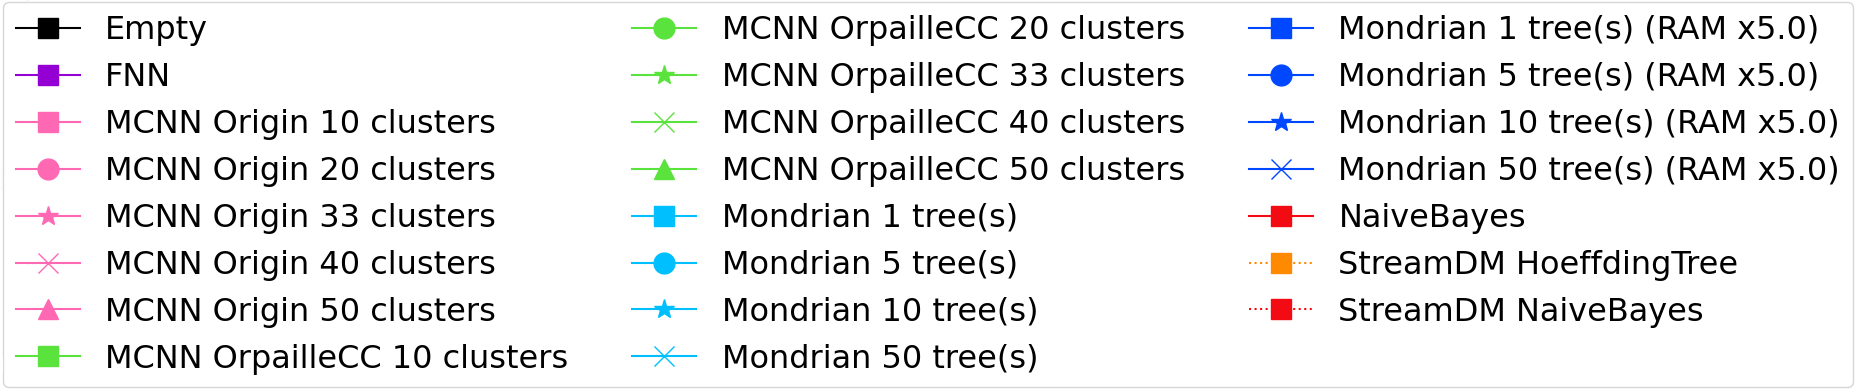
\includegraphics[width=0.8\linewidth]{figures/legend.png}
	\begin{subfigure}[t]{.49\linewidth}
		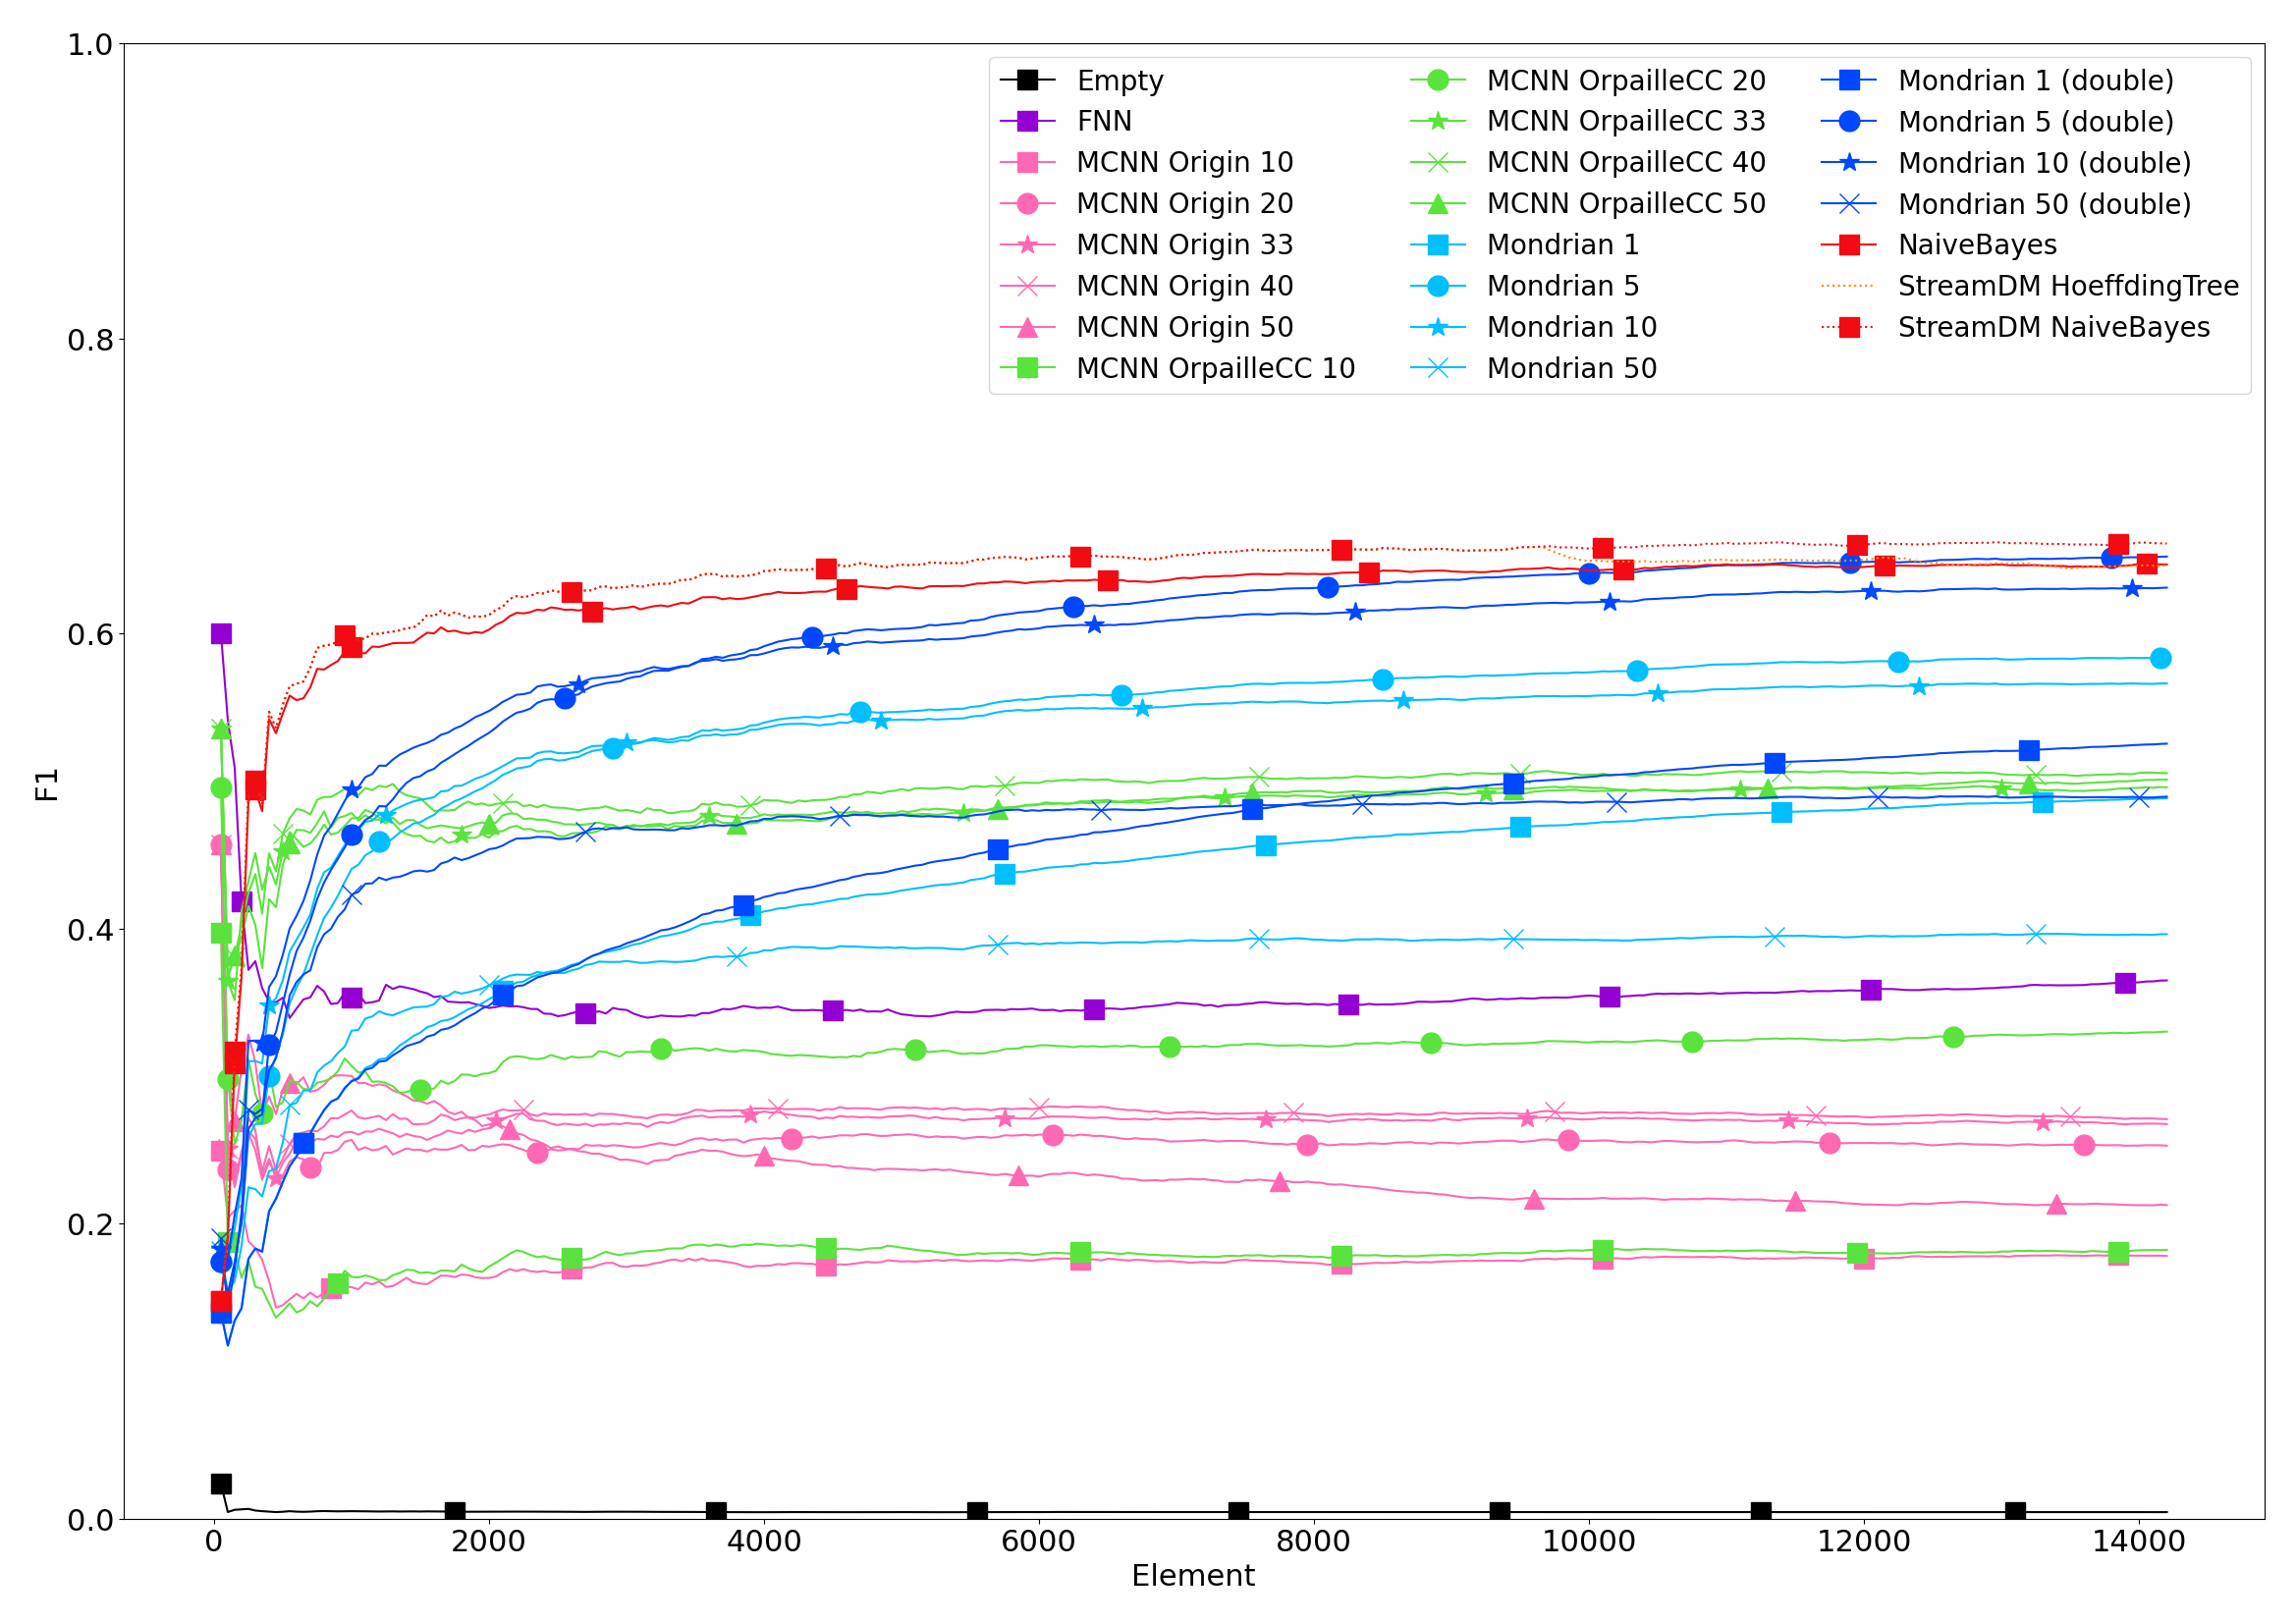
\includegraphics[width=\linewidth]{figures/results/banos_6_f1.png}
		\caption{\banosdataset}
		\label{fig:f1-banos}
	\end{subfigure}
	\begin{subfigure}[t]{.49\linewidth}
		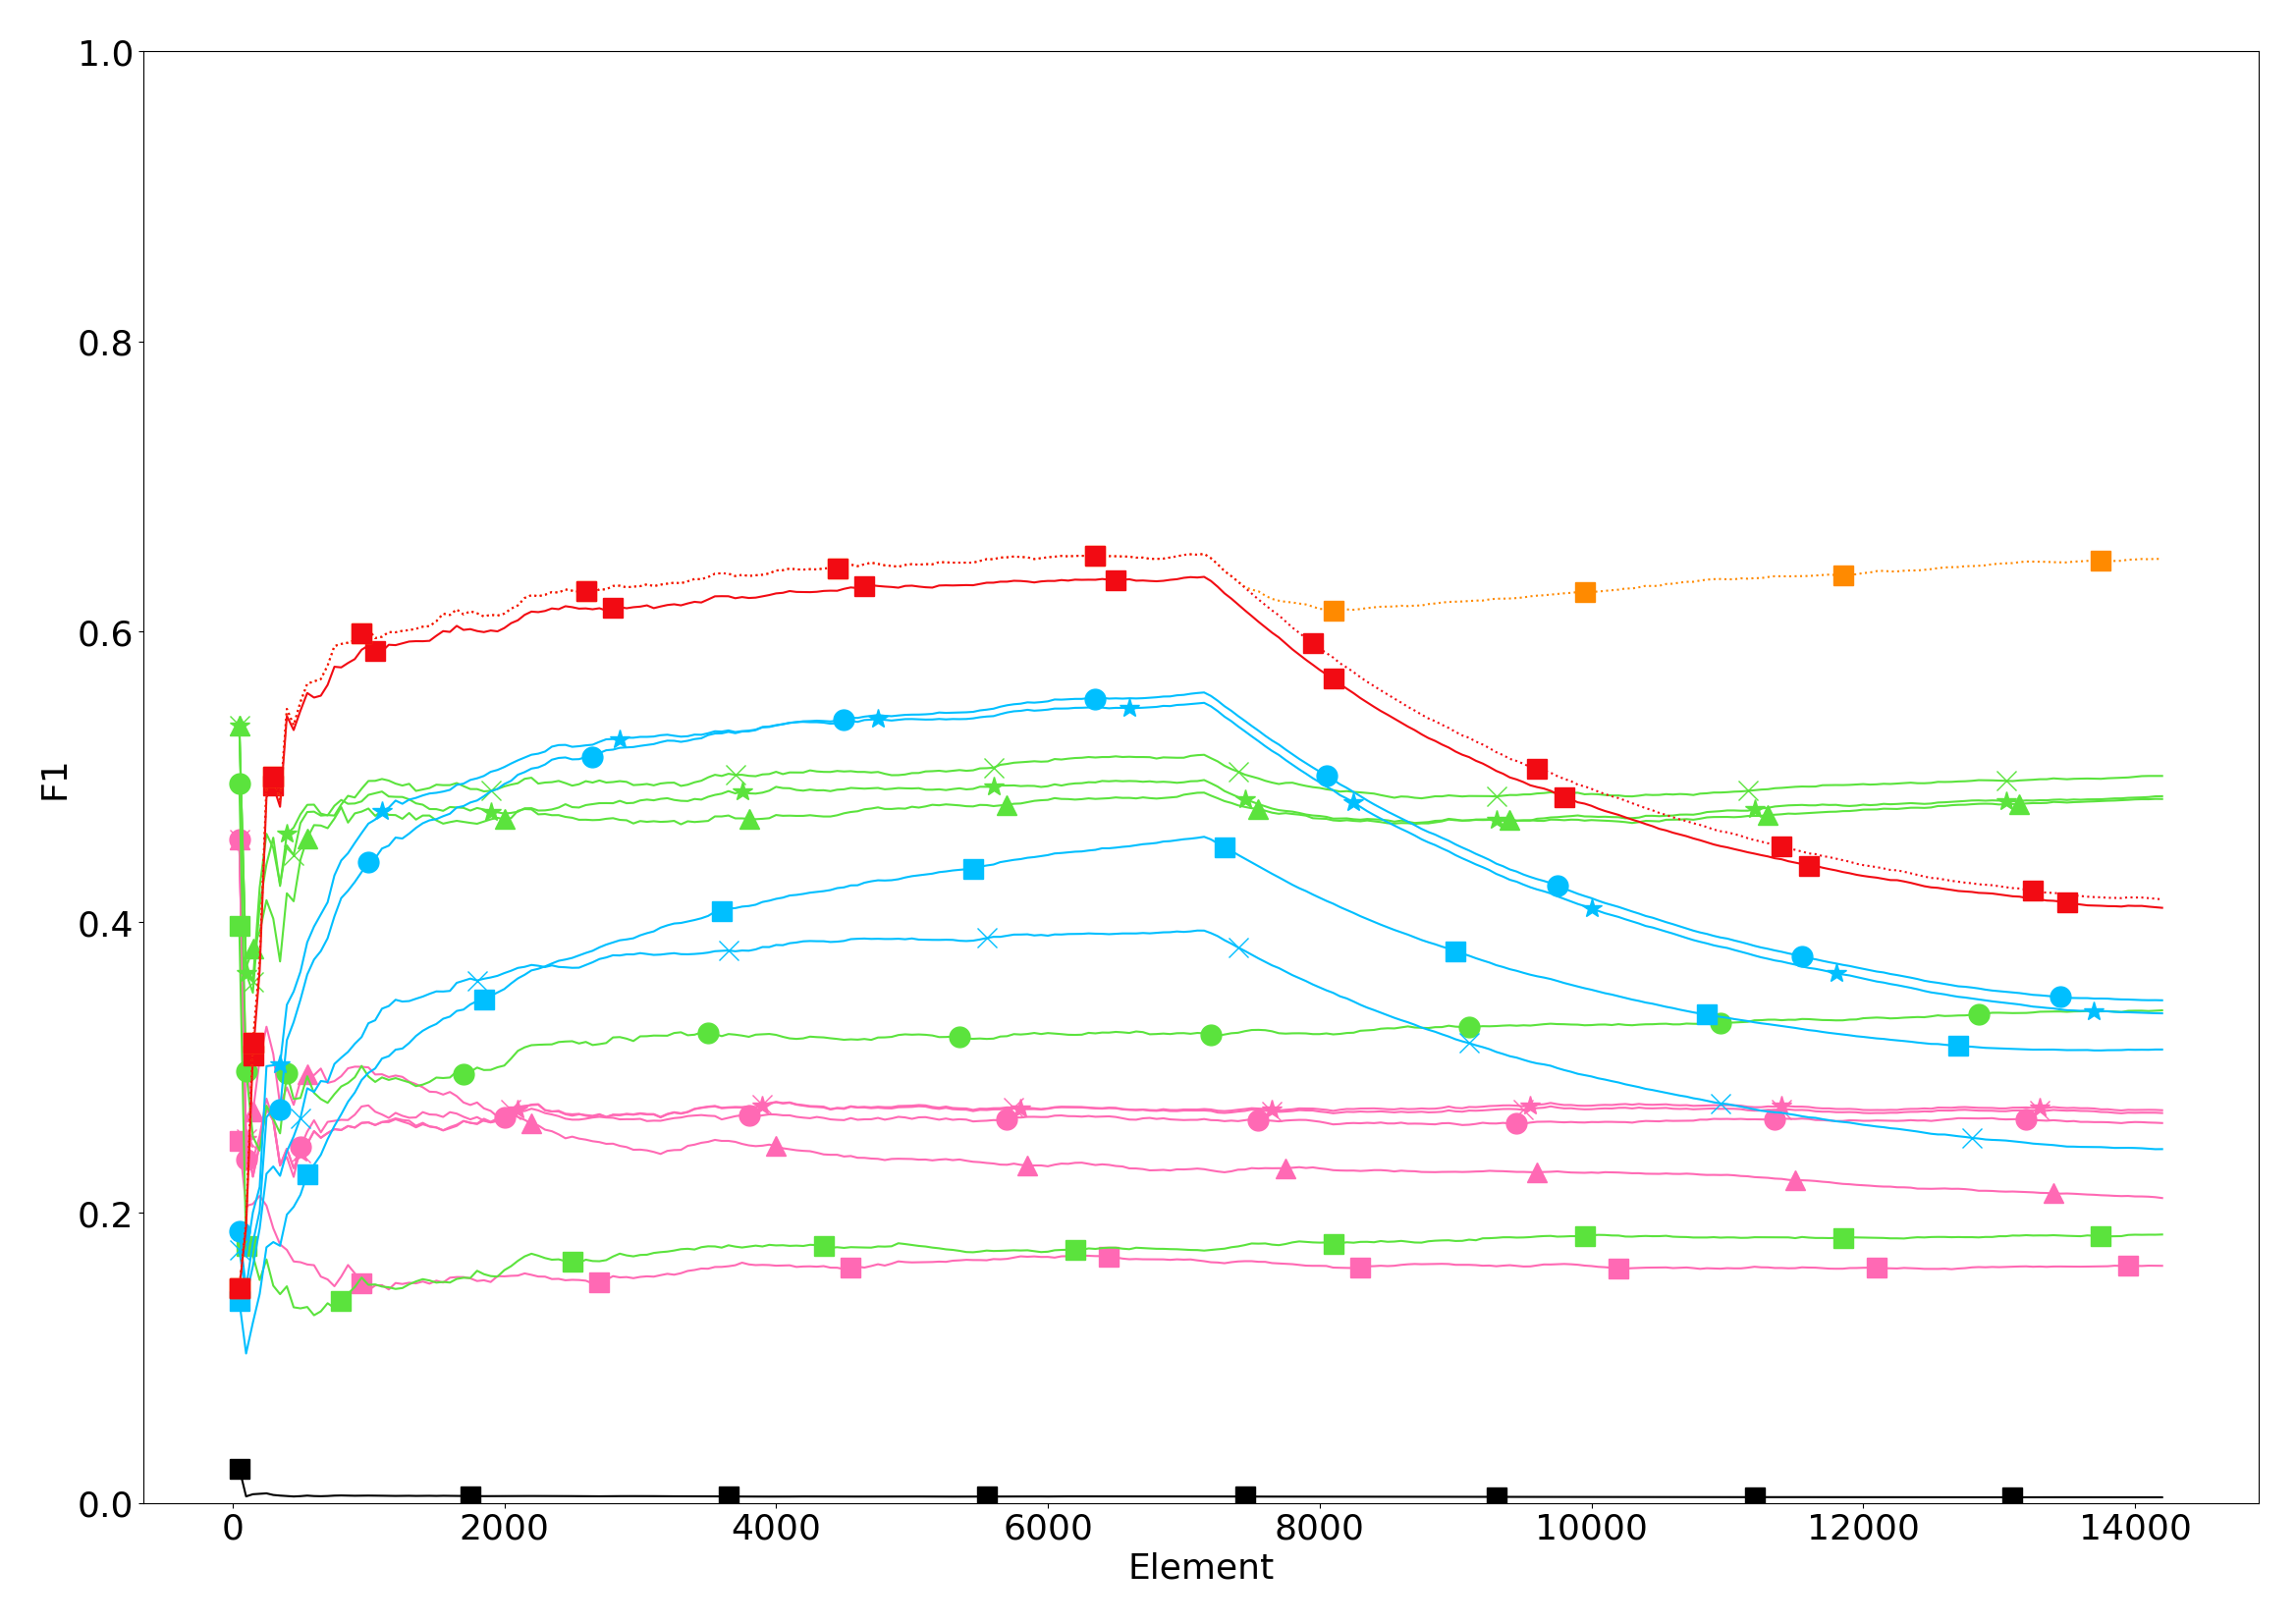
\includegraphics[width=\linewidth]{figures/results/drift_6_f1.png}
		\caption{\banosdataset (with Drift)}
		\label{fig:f1-drift}
	\end{subfigure}\\
	\begin{subfigure}[t]{.49\linewidth}
		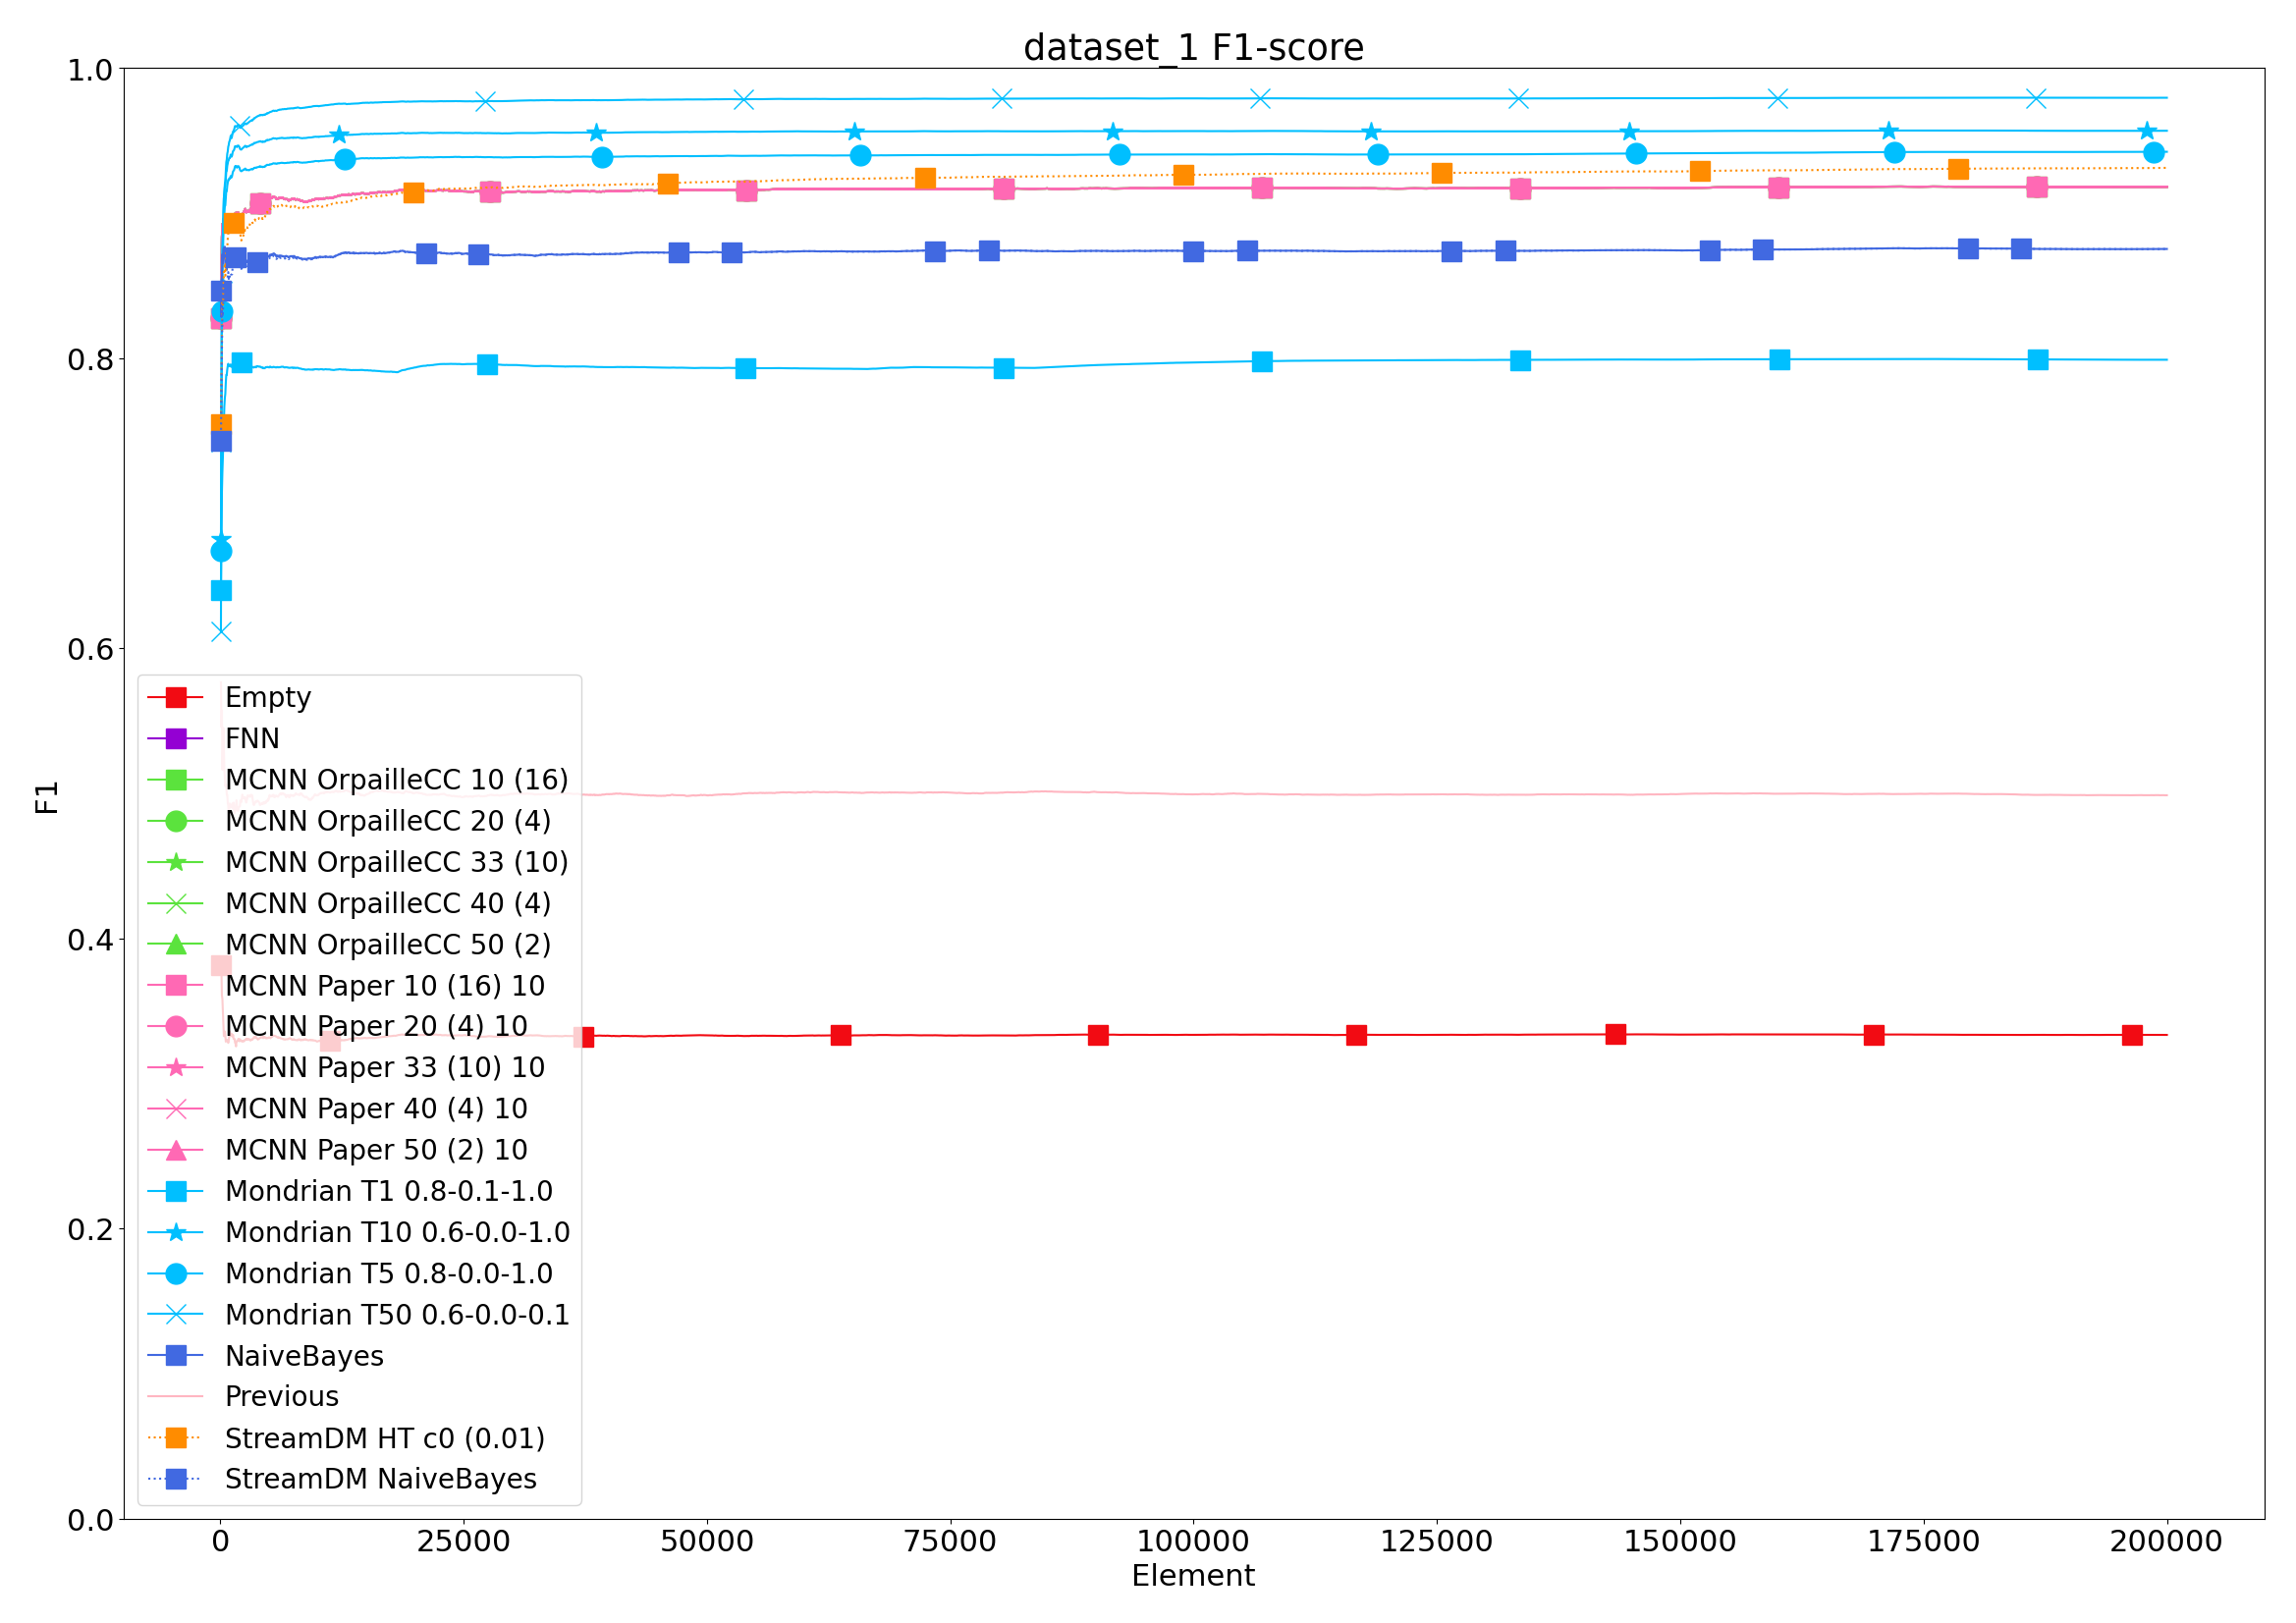
\includegraphics[width=\linewidth]{figures/results/dataset_1_f1.png}
		\caption{Hyperplane (MOA)}
		\label{fig:f1-dataset_1}
	\end{subfigure}
	\begin{subfigure}[t]{.49\linewidth}
		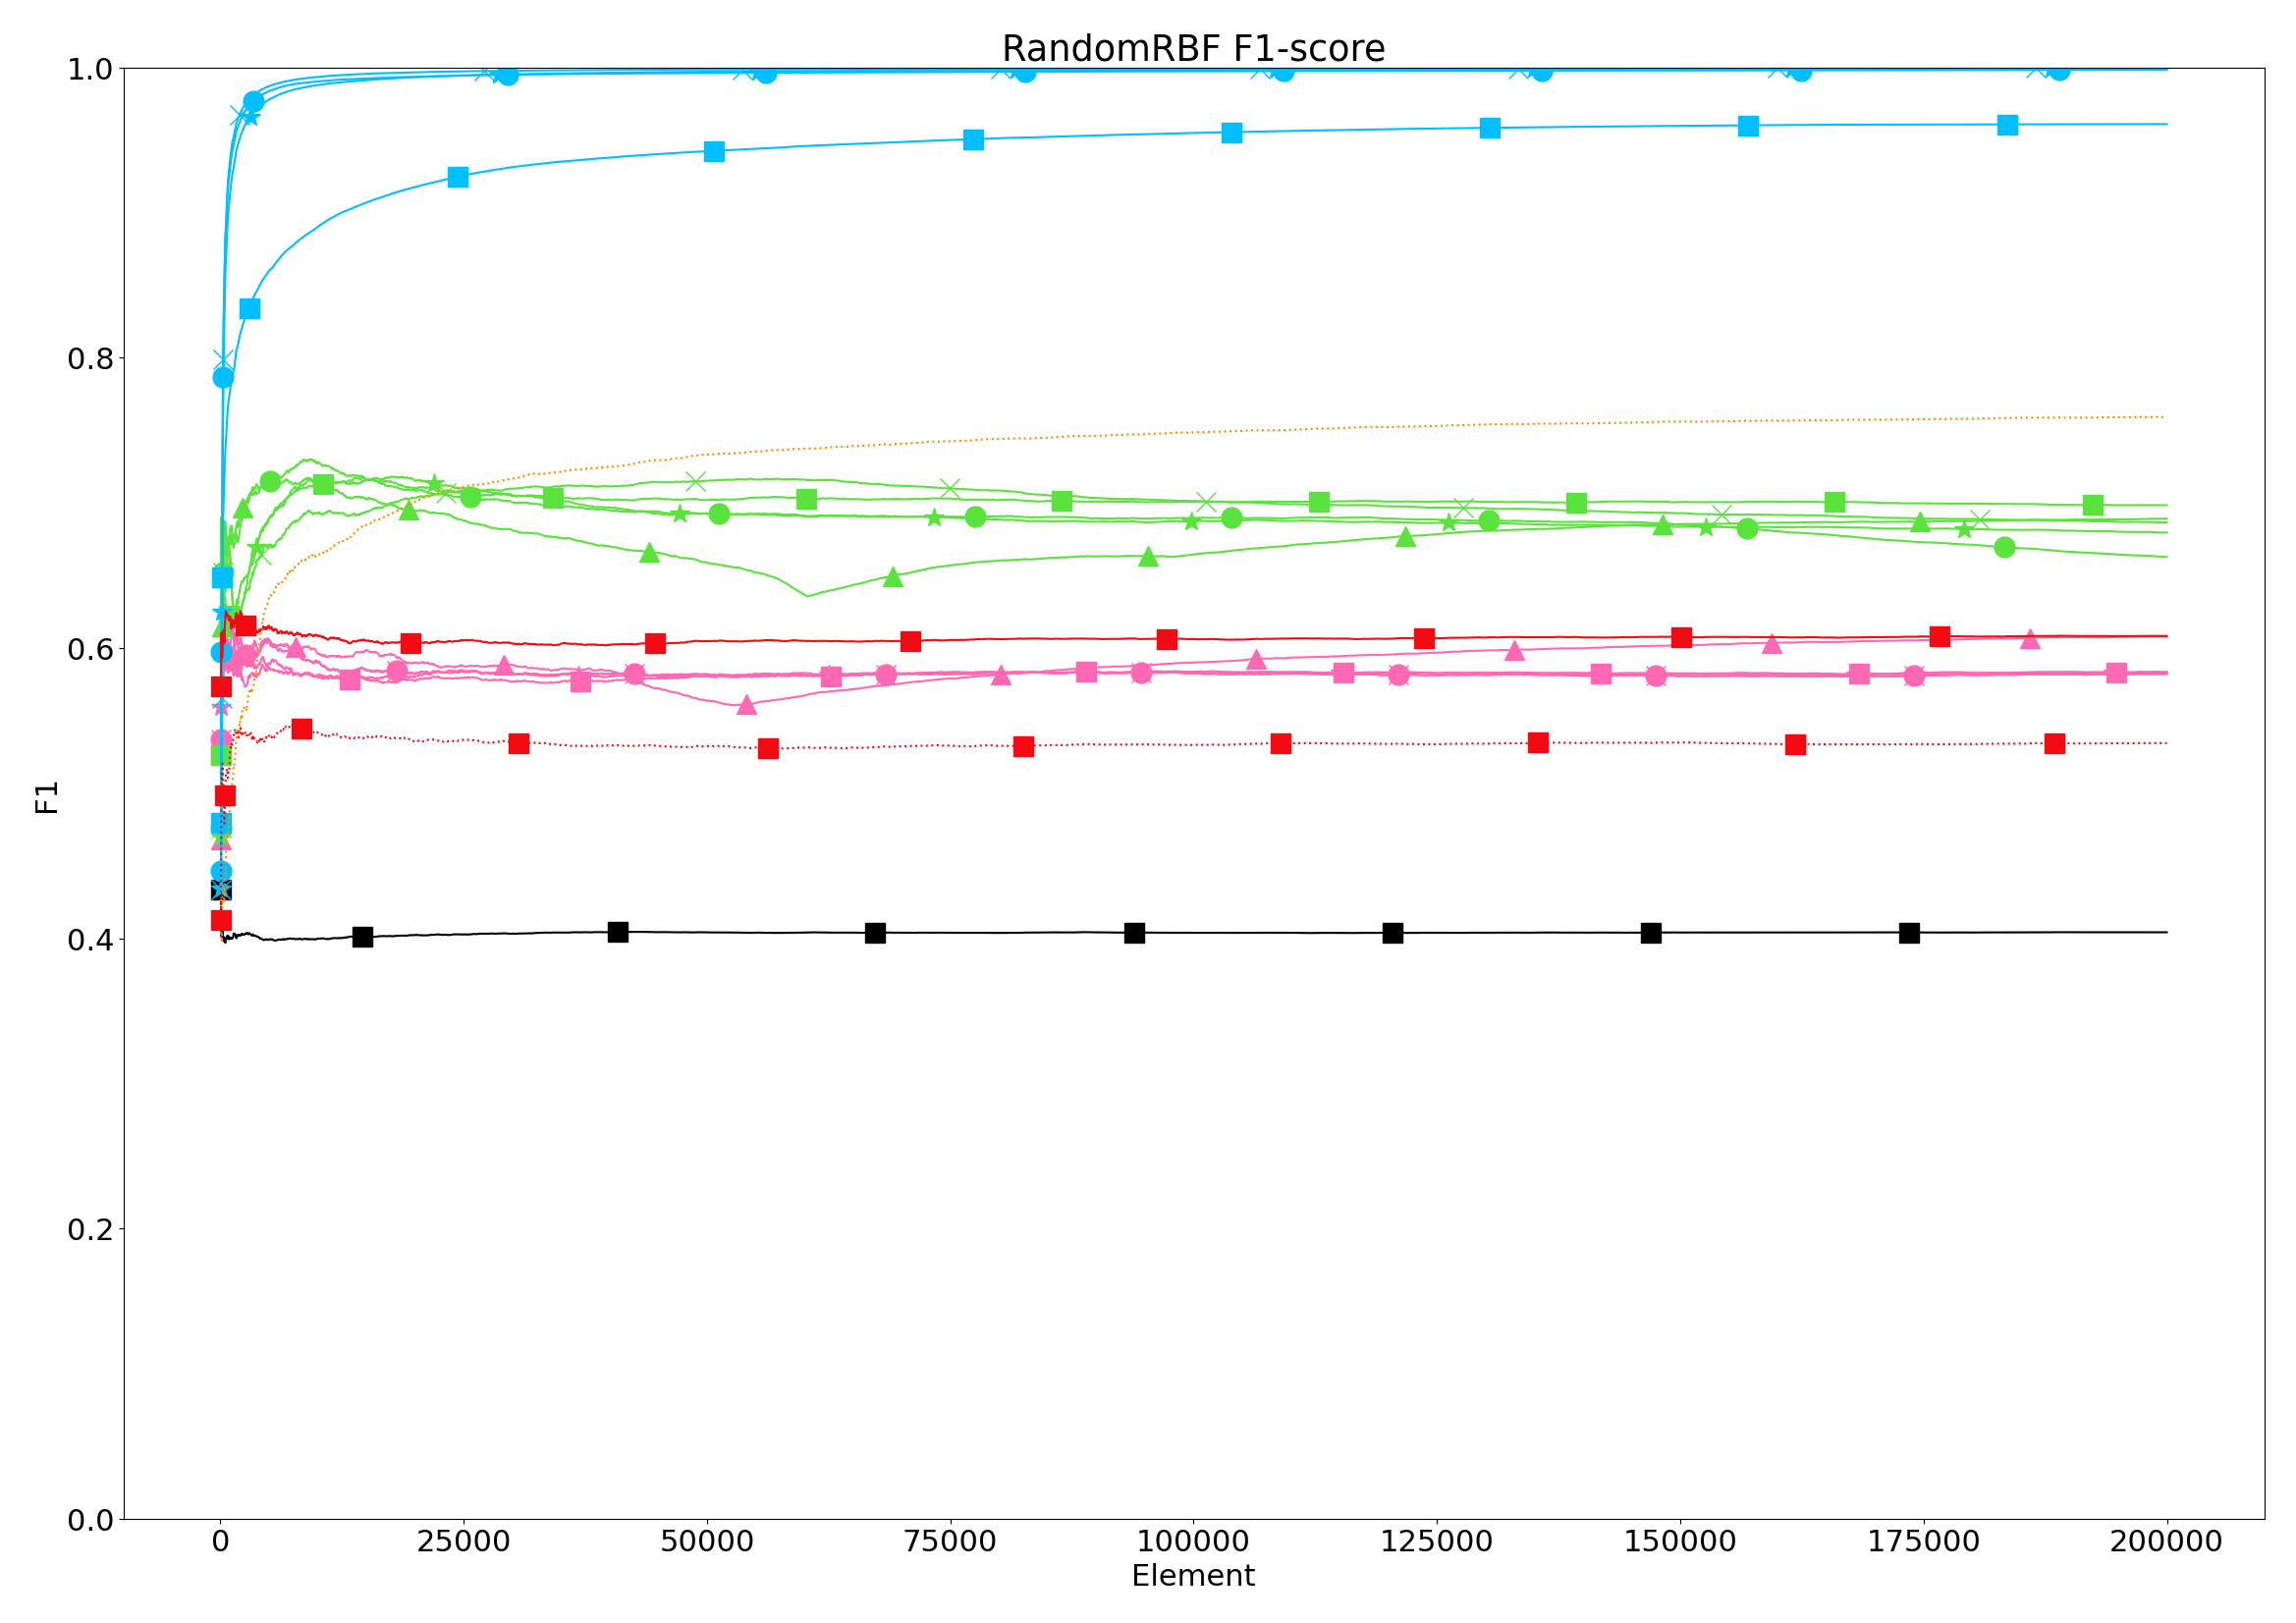
\includegraphics[width=\linewidth]{figures/results/dataset_2_f1.png}
		\caption{RandomRBF (MOA)}
		\label{fig:f1-dataset_2}
	\end{subfigure}\\
	\begin{subfigure}[t]{.49\linewidth}
		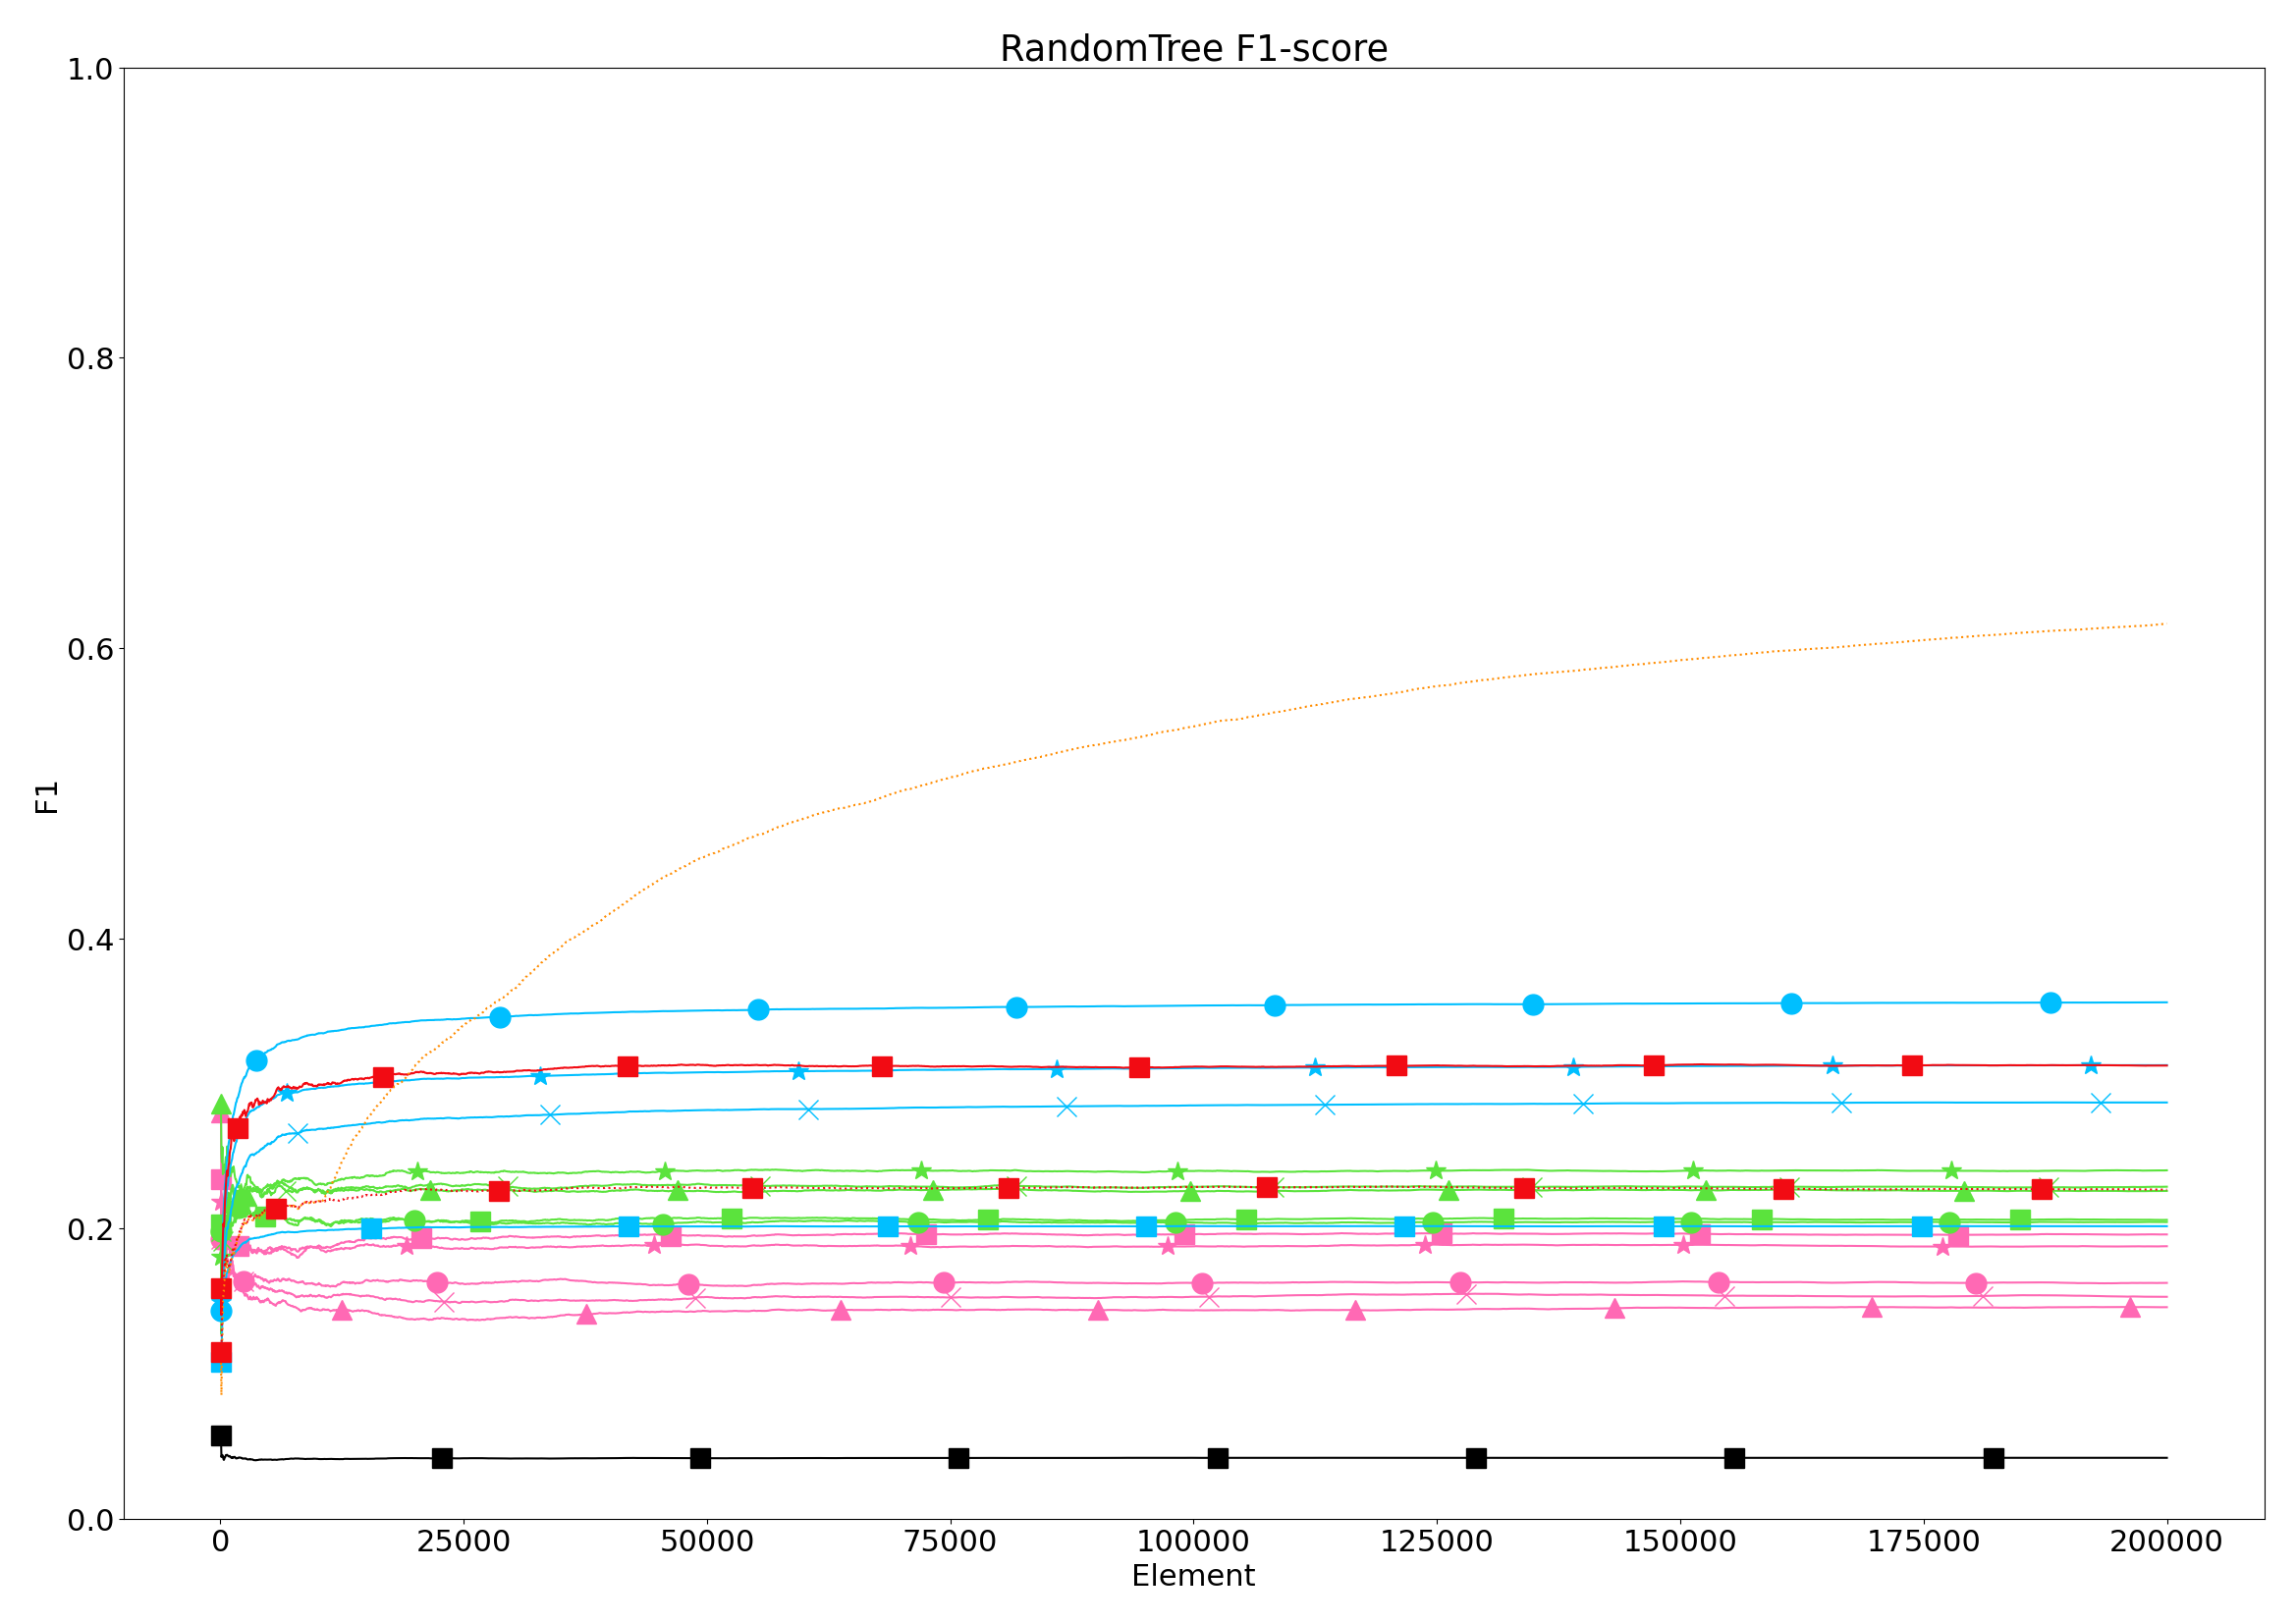
\includegraphics[width=\linewidth]{figures/results/dataset_3_f1.png}
		\caption{RandomTree (MOA)}
		\label{fig:f1-dataset_3}
	\end{subfigure}
	\begin{subfigure}[t]{.49\linewidth}
		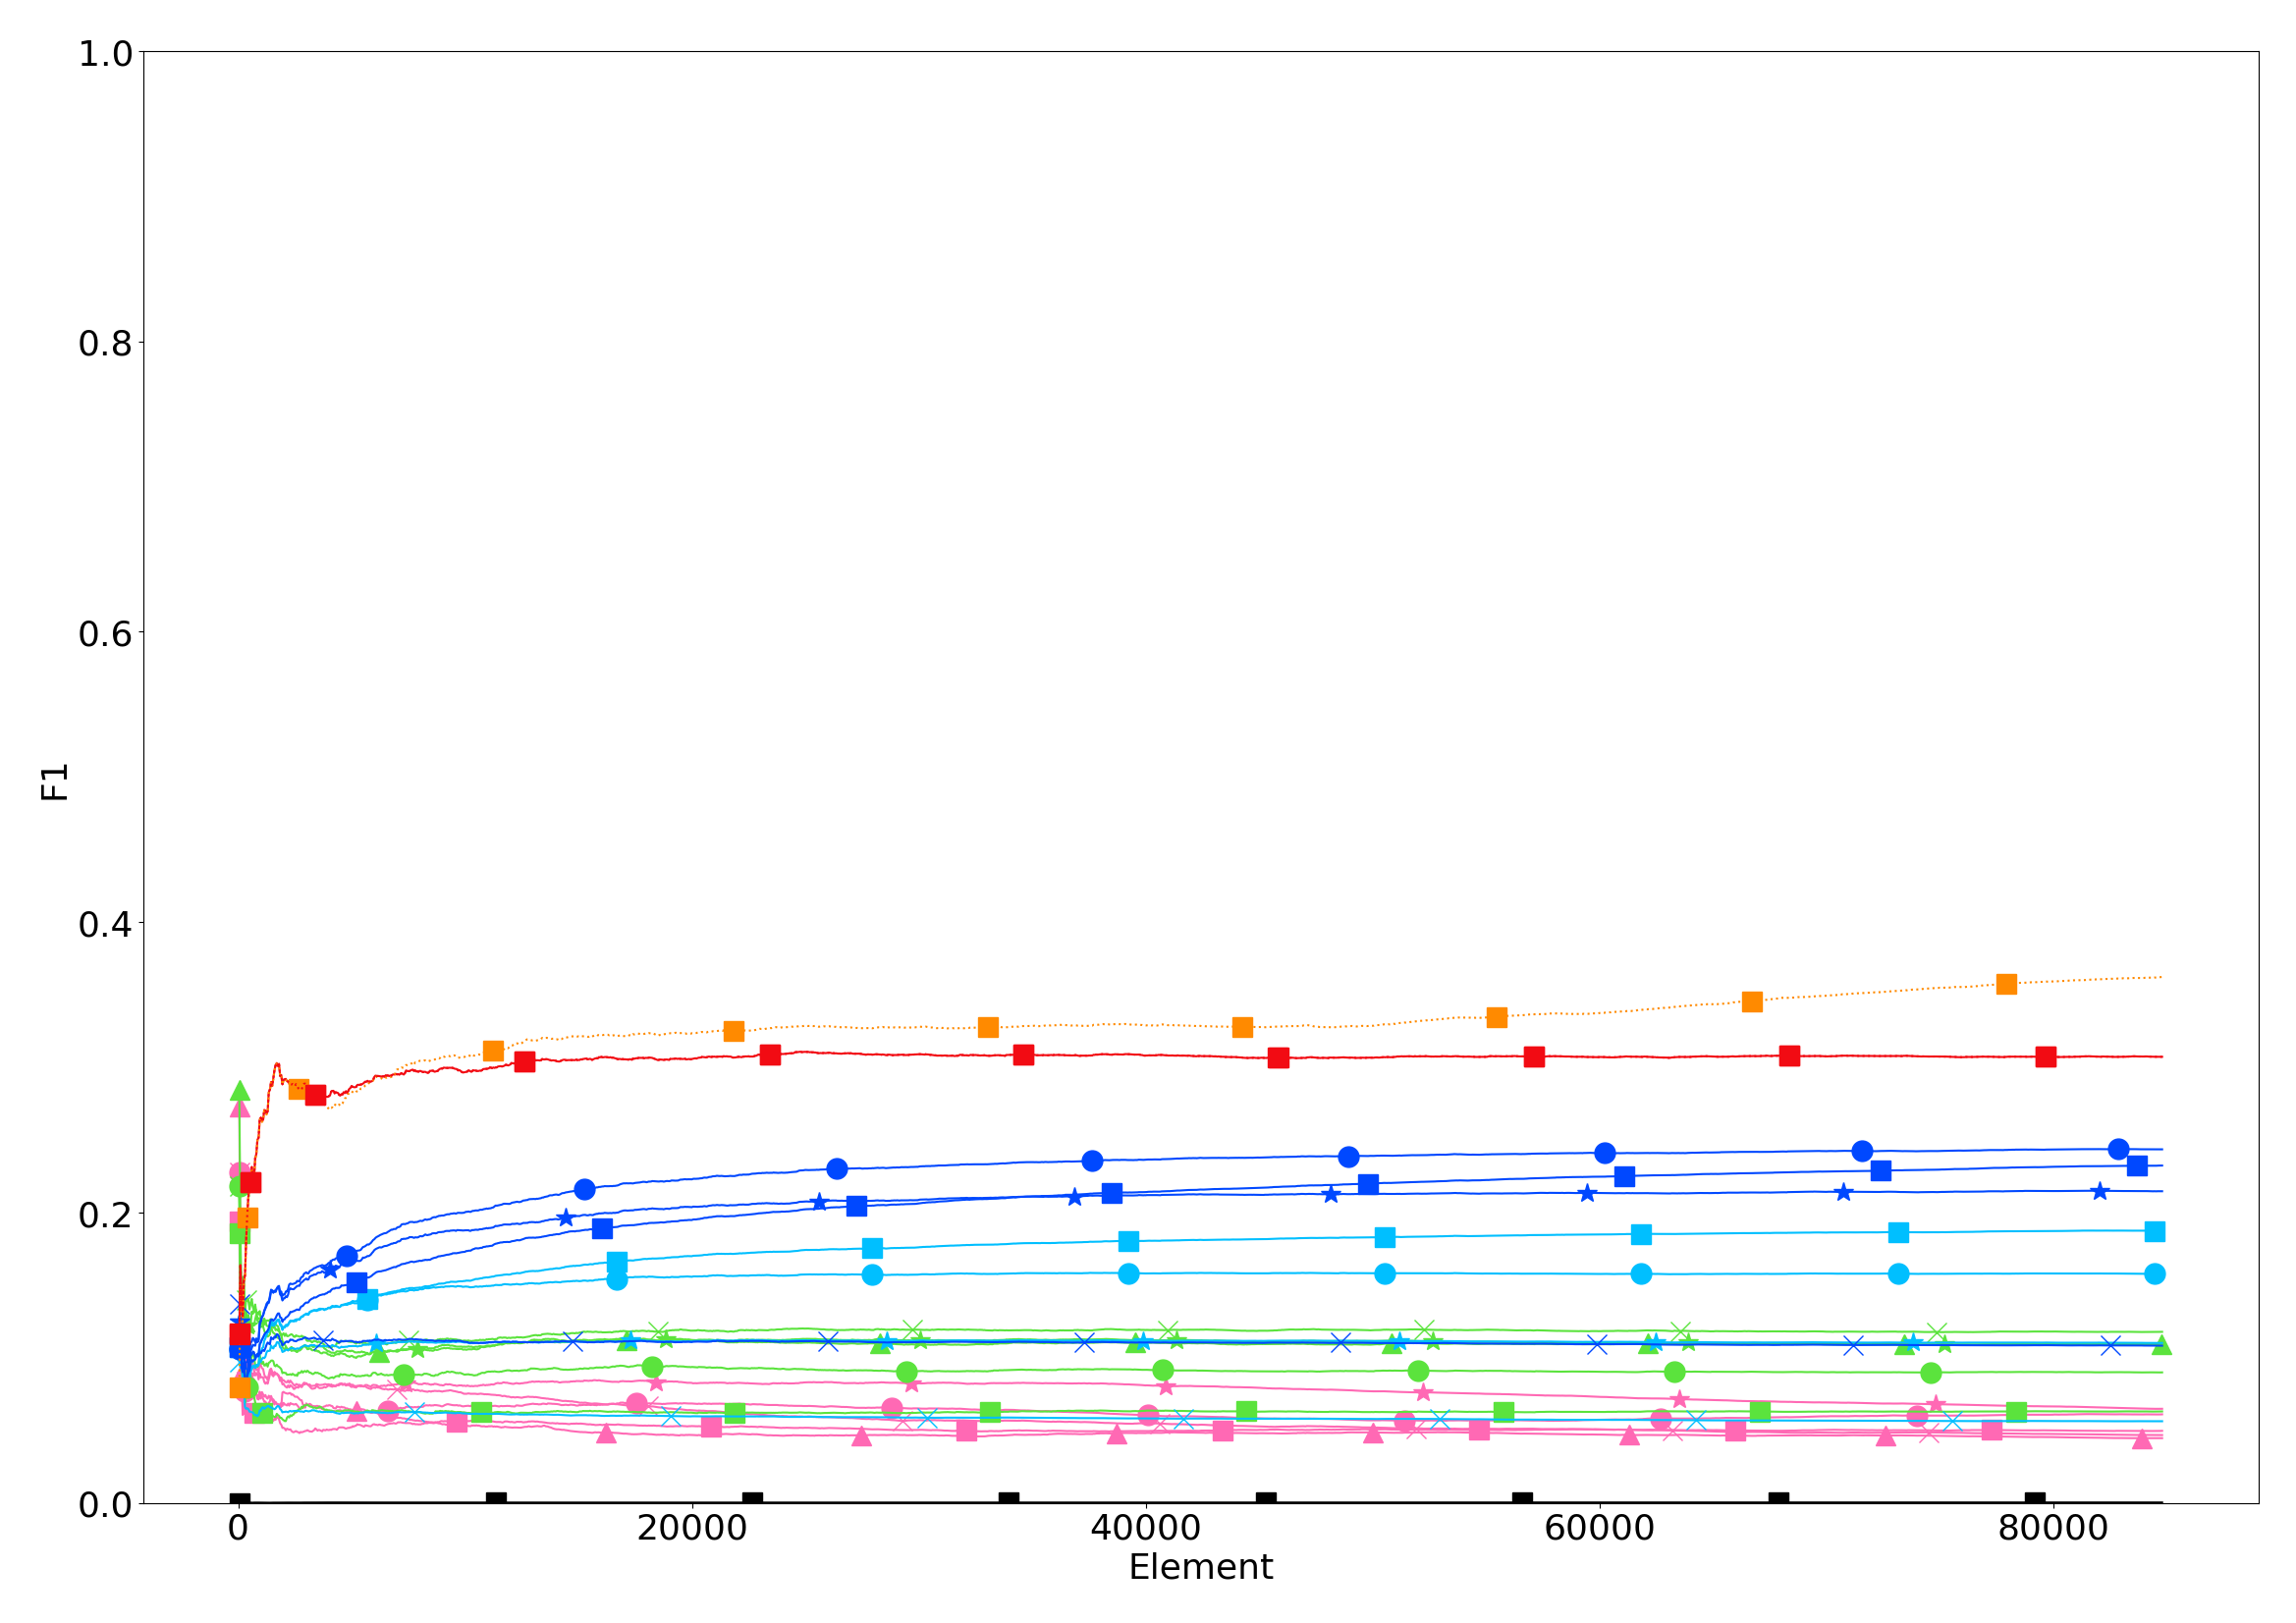
\includegraphics[width=\linewidth]{figures/results/recofit_6_f1.png}
		\caption{\recofitdataset}
		\label{fig:f1-recofit}
	\end{subfigure}
	\caption{F1-scores for the six datasets (average over 20 repetitions).}
	\label{fig:f1}
\end{figure*}

\section{Results}
This section presents our benchmark results and the corresponding
hyperparameter tunning experiments.

\subsection{F1-score}
Figure~\ref{fig:f1} compares the F1-scores obtained by all classifiers on the
six datasets.
\naivebayes and the \hoeffdingtree outperform the other classifiers on the two
real datasets (\banosdataset and \recofitdataset) even though the F1-scores
observed remained low (0.6 and 0.35) compared to offline results (0.92 and
0.7)~\cite{behzad2019} \TG{OK but these results used more than 1 sensor, it would be better to do the offline experiment yourself}.  On the other hand, the \mondrianforest with 5 or 10
trees achieves the best performances on 2 synthetic datasets.  The
\mondrianforest \TG{mention with how much RAM because it is ambiguous} is also the third classifier on the two real datasets.  Finally, the
\hoeffdingtree outperforms all other classifiers on the RandomTree dataset,
where it is followed by the \mondrianforest.
\TG{Methods should explain how much RAM were given to Mondrian forest, and explain that for some datasets 
you also used RAM x 5.}

F1-score values vary greatly across the datasets.  While the highest
observed F1-score is above 0.95 on the Hyperplane and RandomRBF datasets,
it barely reaches 0.65 for the \banosdataset dataset, and it remains under
0.4 on the \recofitdataset and RandomTree datasets. This trend is
consistent for all classifiers.

The StreamDM \hoeffdingtree algorithm achieves better performance than the
\naivebayes except for the \banosdataset dataset.  Both of them start close
together because the \hoeffdingtree uses a \naivebayes in its leaves.  However,
they start diverging because the \hoeffdingtree improves by reshaping its tree
structure.  This is caused by a sufficient amount of element and the difference
is more noticable when a concept drift occurs \TG{do you have evidence for the 
affirmations of the last two sentences? If not, let's just write ``most likely because'' or ``presumably due to''.}.

On all datasets, \mcnn OrpailleCC achieves better performances than \mcnn
Original. Additionally, on the RandomRBF and RandomTree datasets, the lowest
\mcnn OrpailleCC performs better than the highest \mcnn Origin \TG{not sure what this means, fix syntax}. Presumably due
to the fact that \mcnn Original removes clusters too fast even with the
participation threshold low \TG{This sentence lacks a verb}.
Besides, on the real datasets (\banosdataset and \recofitdataset), the \mcnn OrpailleCC
classifier appears to be learning faster than the \mondrianforest, although
\mondrianforest catches up after a few thousand elements. 

Surprisingly, a \mondrianforest with 50 trees performs worse than with 5 or
10 trees \TG{on all datasets?}. This is due to the fact that our
\mondrianforest implementation allocates a fixed amount of memory, which is
useful on connected objects but limits tree growth when the allocated
memory is full. Because 50 trees fill the memory faster than 10 or 5 trees,
the classifier adaptation is blocked faster, when the trees have not
learned enough from the data.

This dependency of the \mondrianforest to memory allocation is 
shown in Figures~\ref{fig:f1-banos}-\ref{fig:f1-recofit}, where 
an additional configuration with twice as much memory as the base one is shown.
The memory increase induces a F1-score difference greater than 0.1, except when only one tree
is used. In which case the improvement caused by the memory is less than 0.05 \TG{this sentence lacks a verb}.

The \hoeffdingtree appears to be the most robust to concept drifts
(Figure~\ref{fig:f1-drift}), while the \mondrianforest and \naivebayes
classifiers are the most impacted. \mcnn classifiers are only marginally impacted.
The low resilience of \mondrianforest to concept drifts can be attributed to
two factors. First, existing nodes in trees of a \mondrianforest cannot be updated.
Second, when the memory limit is reached, \mondrianforest cannot grow
or reshape their structure anymore.

\begin{figure}
		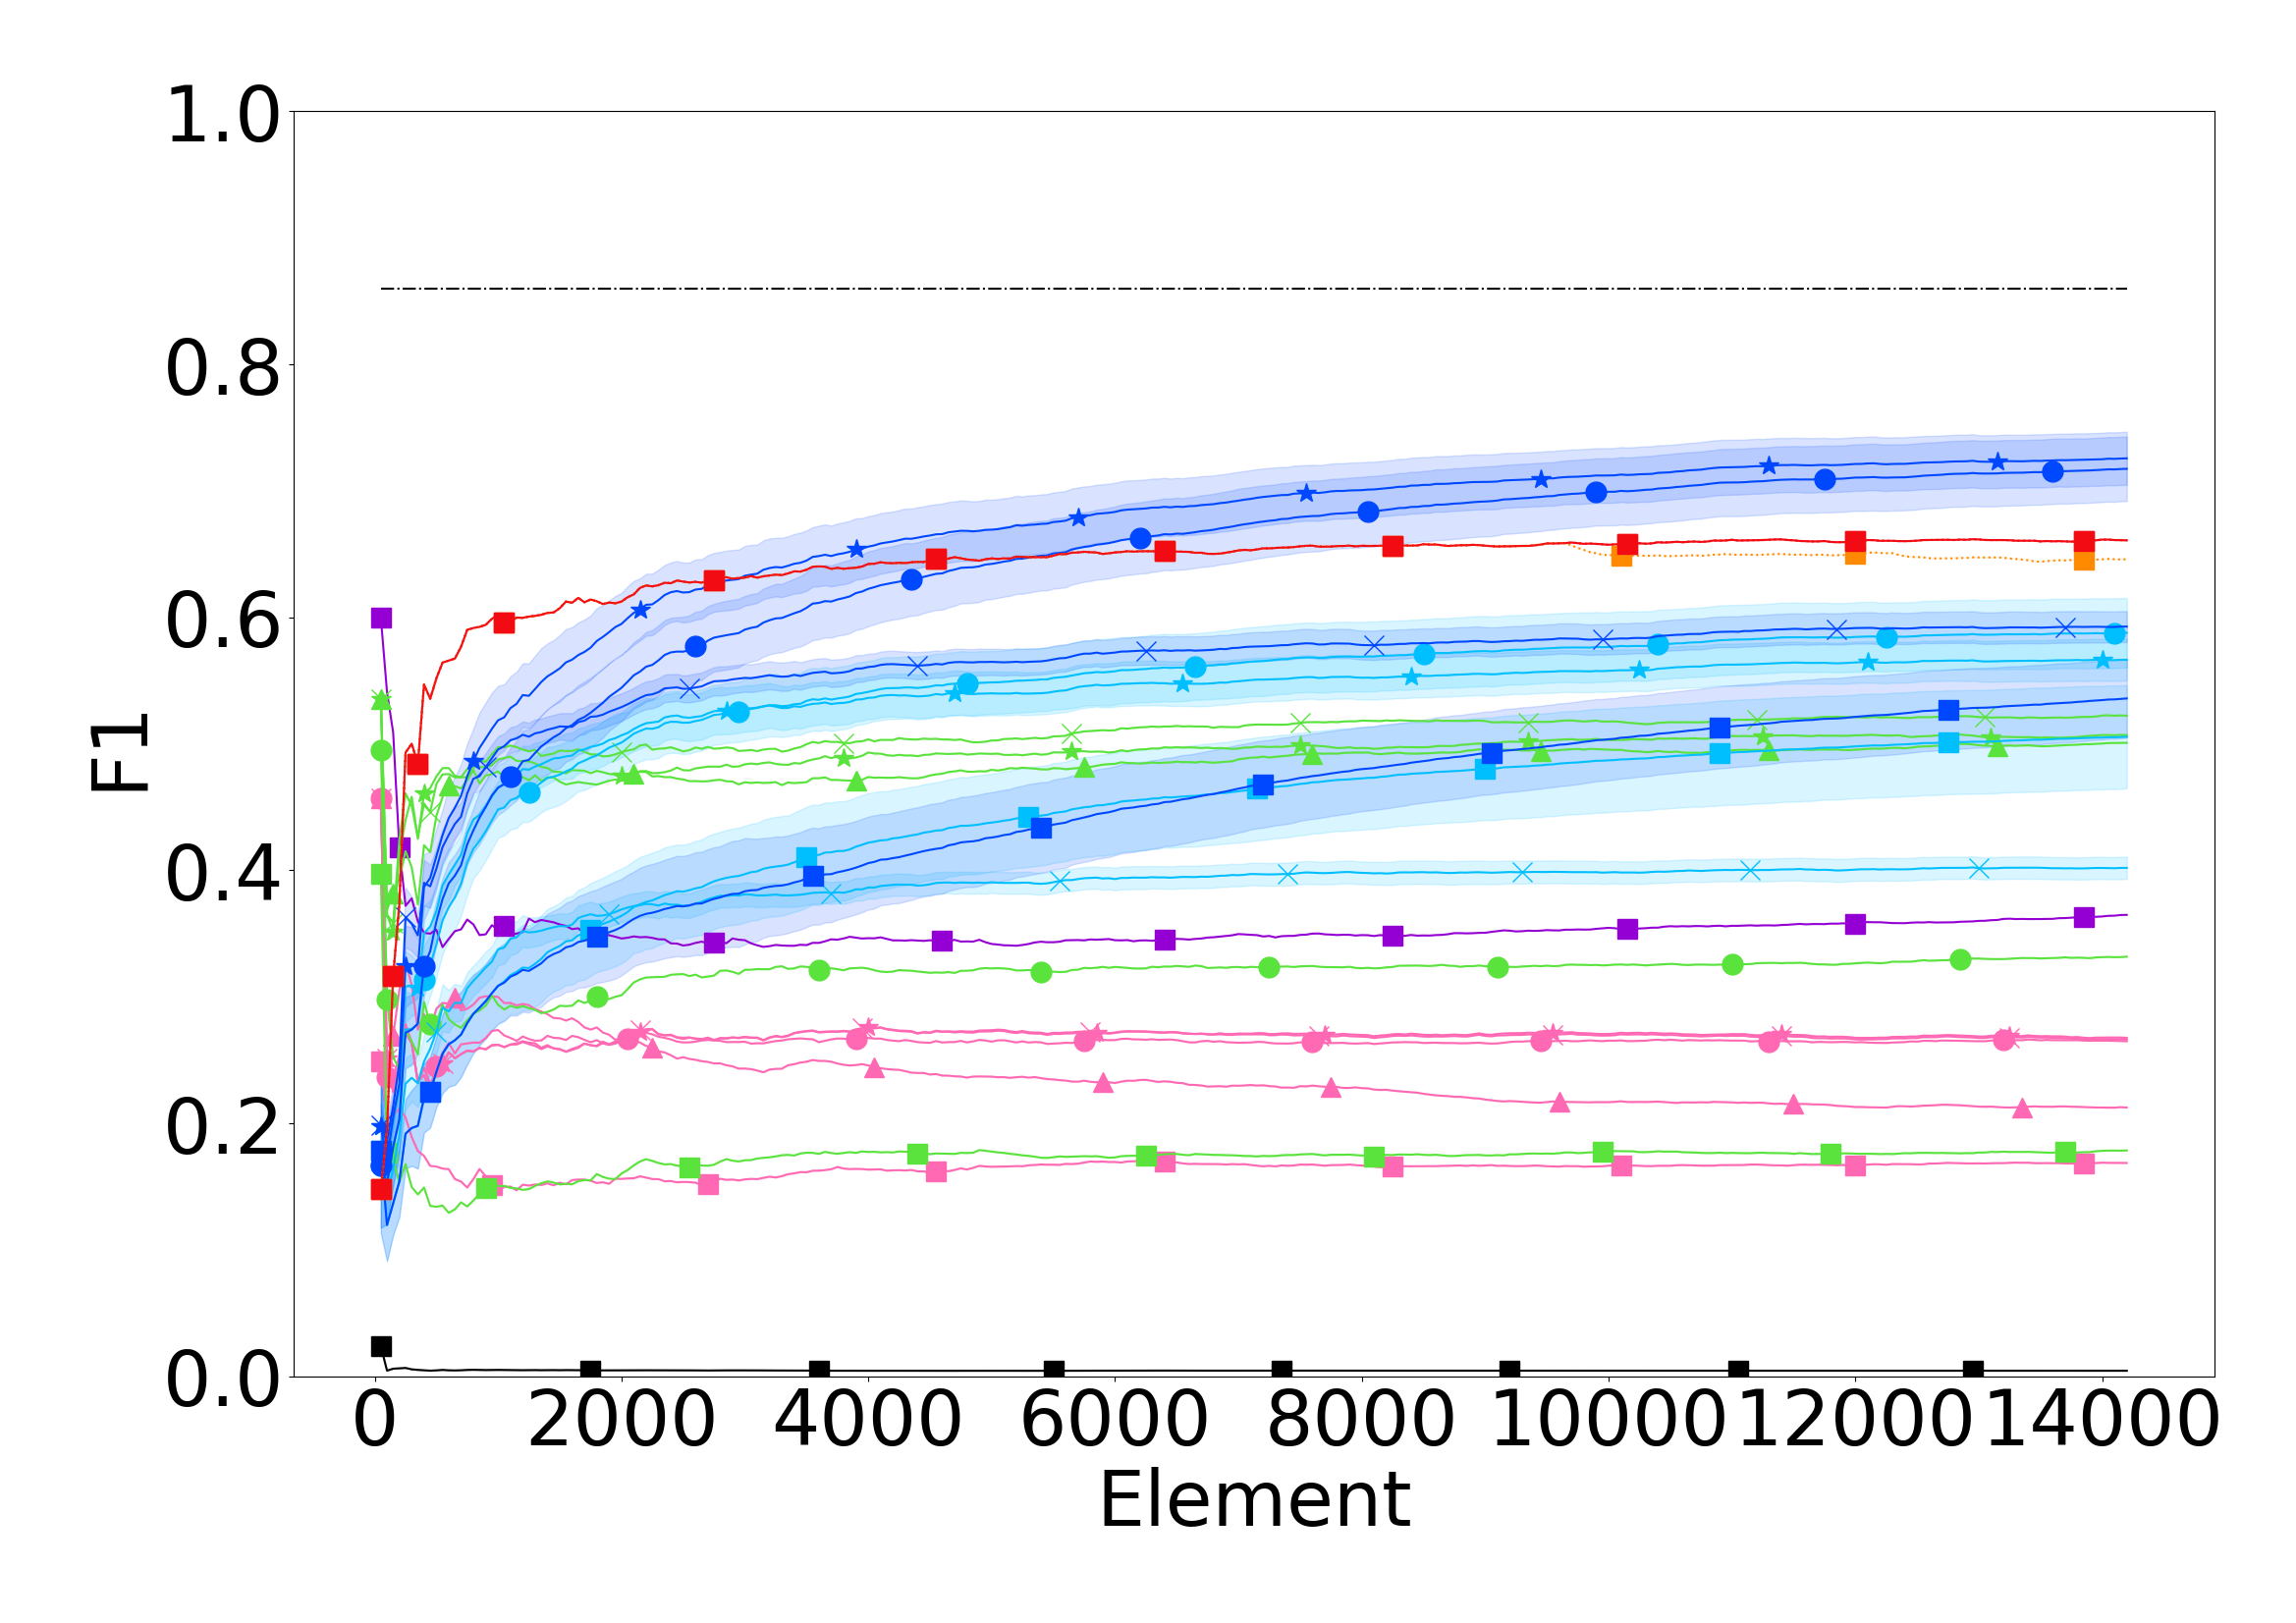
\includegraphics[width=\linewidth]{figures/results/banos_6_f1_std.png}
		\caption{F1-score variance on \banosdataset dataset. Some classifiers
		have been removed to make the Figure clearer (\mcnn Origin,
		\hoeffdingtree, some of the \mcnn OrpailleCC)}
		\label{fig:f1-variance}
\end{figure}

Figure~\ref{fig:f1-variance} shows the variance of the F1-score for
\mondrianforest classifiers, the only ones to involve randomness. The
variance decreases with the number of trees, as expected. We notice that
the \mondrianforest variance with double memory covers the \naivebayes
lines. Therefore, some \mondrianforest run achieves better F1-score than
the \naivebayes \TG{I dont find the last two sentences particularly
informative and this figure doesn't bring much at the end of the day. Could
you just add variance to figure 3?}.

Figure~\ref{fig:f1-banos} shows that the F1-score of the \FNN
is around 0.3 \TG{Why isn't it shown in the other figures?}. Therefore, it remains better than \mcnn Origin but it is quite
low compare to other classifiers with the same dataset. \TG{Move this to one sentence in the first paragraph of III.A}

Finally, we note that the StreamDM and OrpailleCC implementations of
\naivebayes are indistinguishable from each other, which confirms our
implementation in OrpailleCC.

\begin{figure*}
	\begin{subfigure}[t]{.49\linewidth}
		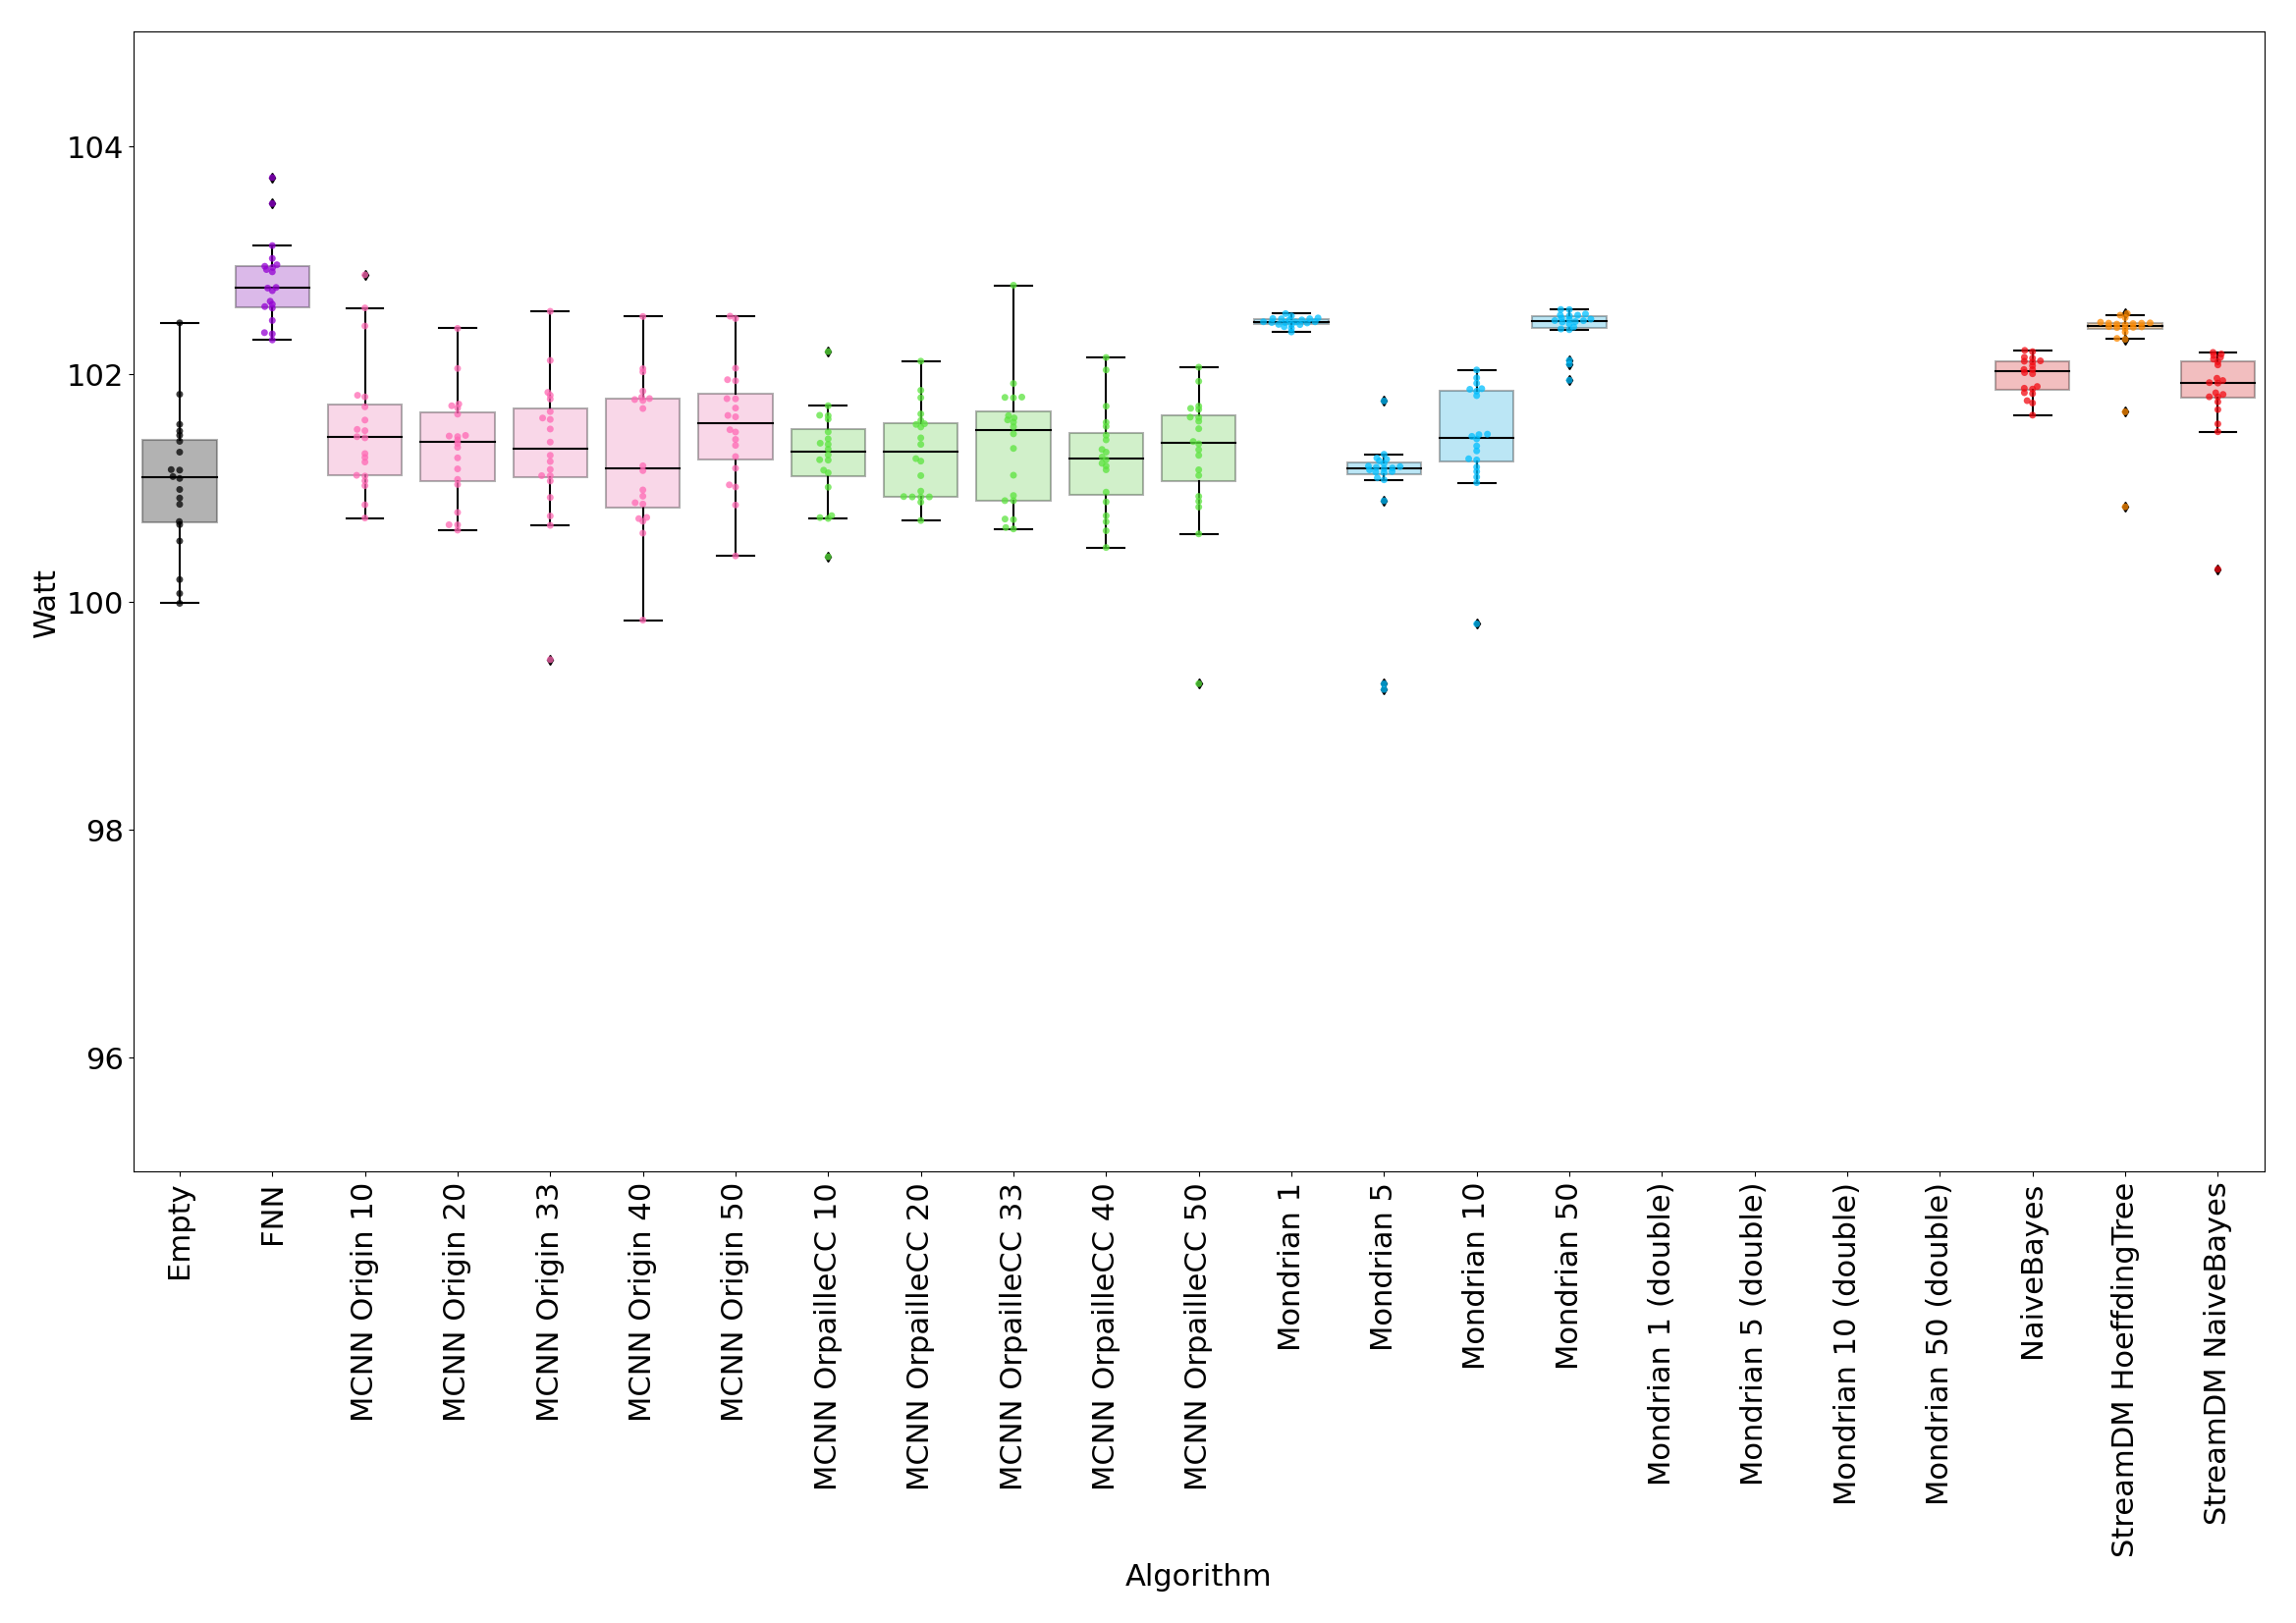
\includegraphics[width=\linewidth]{figures/results/banos_3_watt.png}
		\caption{\banosdataset}
		\label{fig:power-banos}
	\end{subfigure}
	\hfill
	\begin{subfigure}[t]{.49\linewidth}
		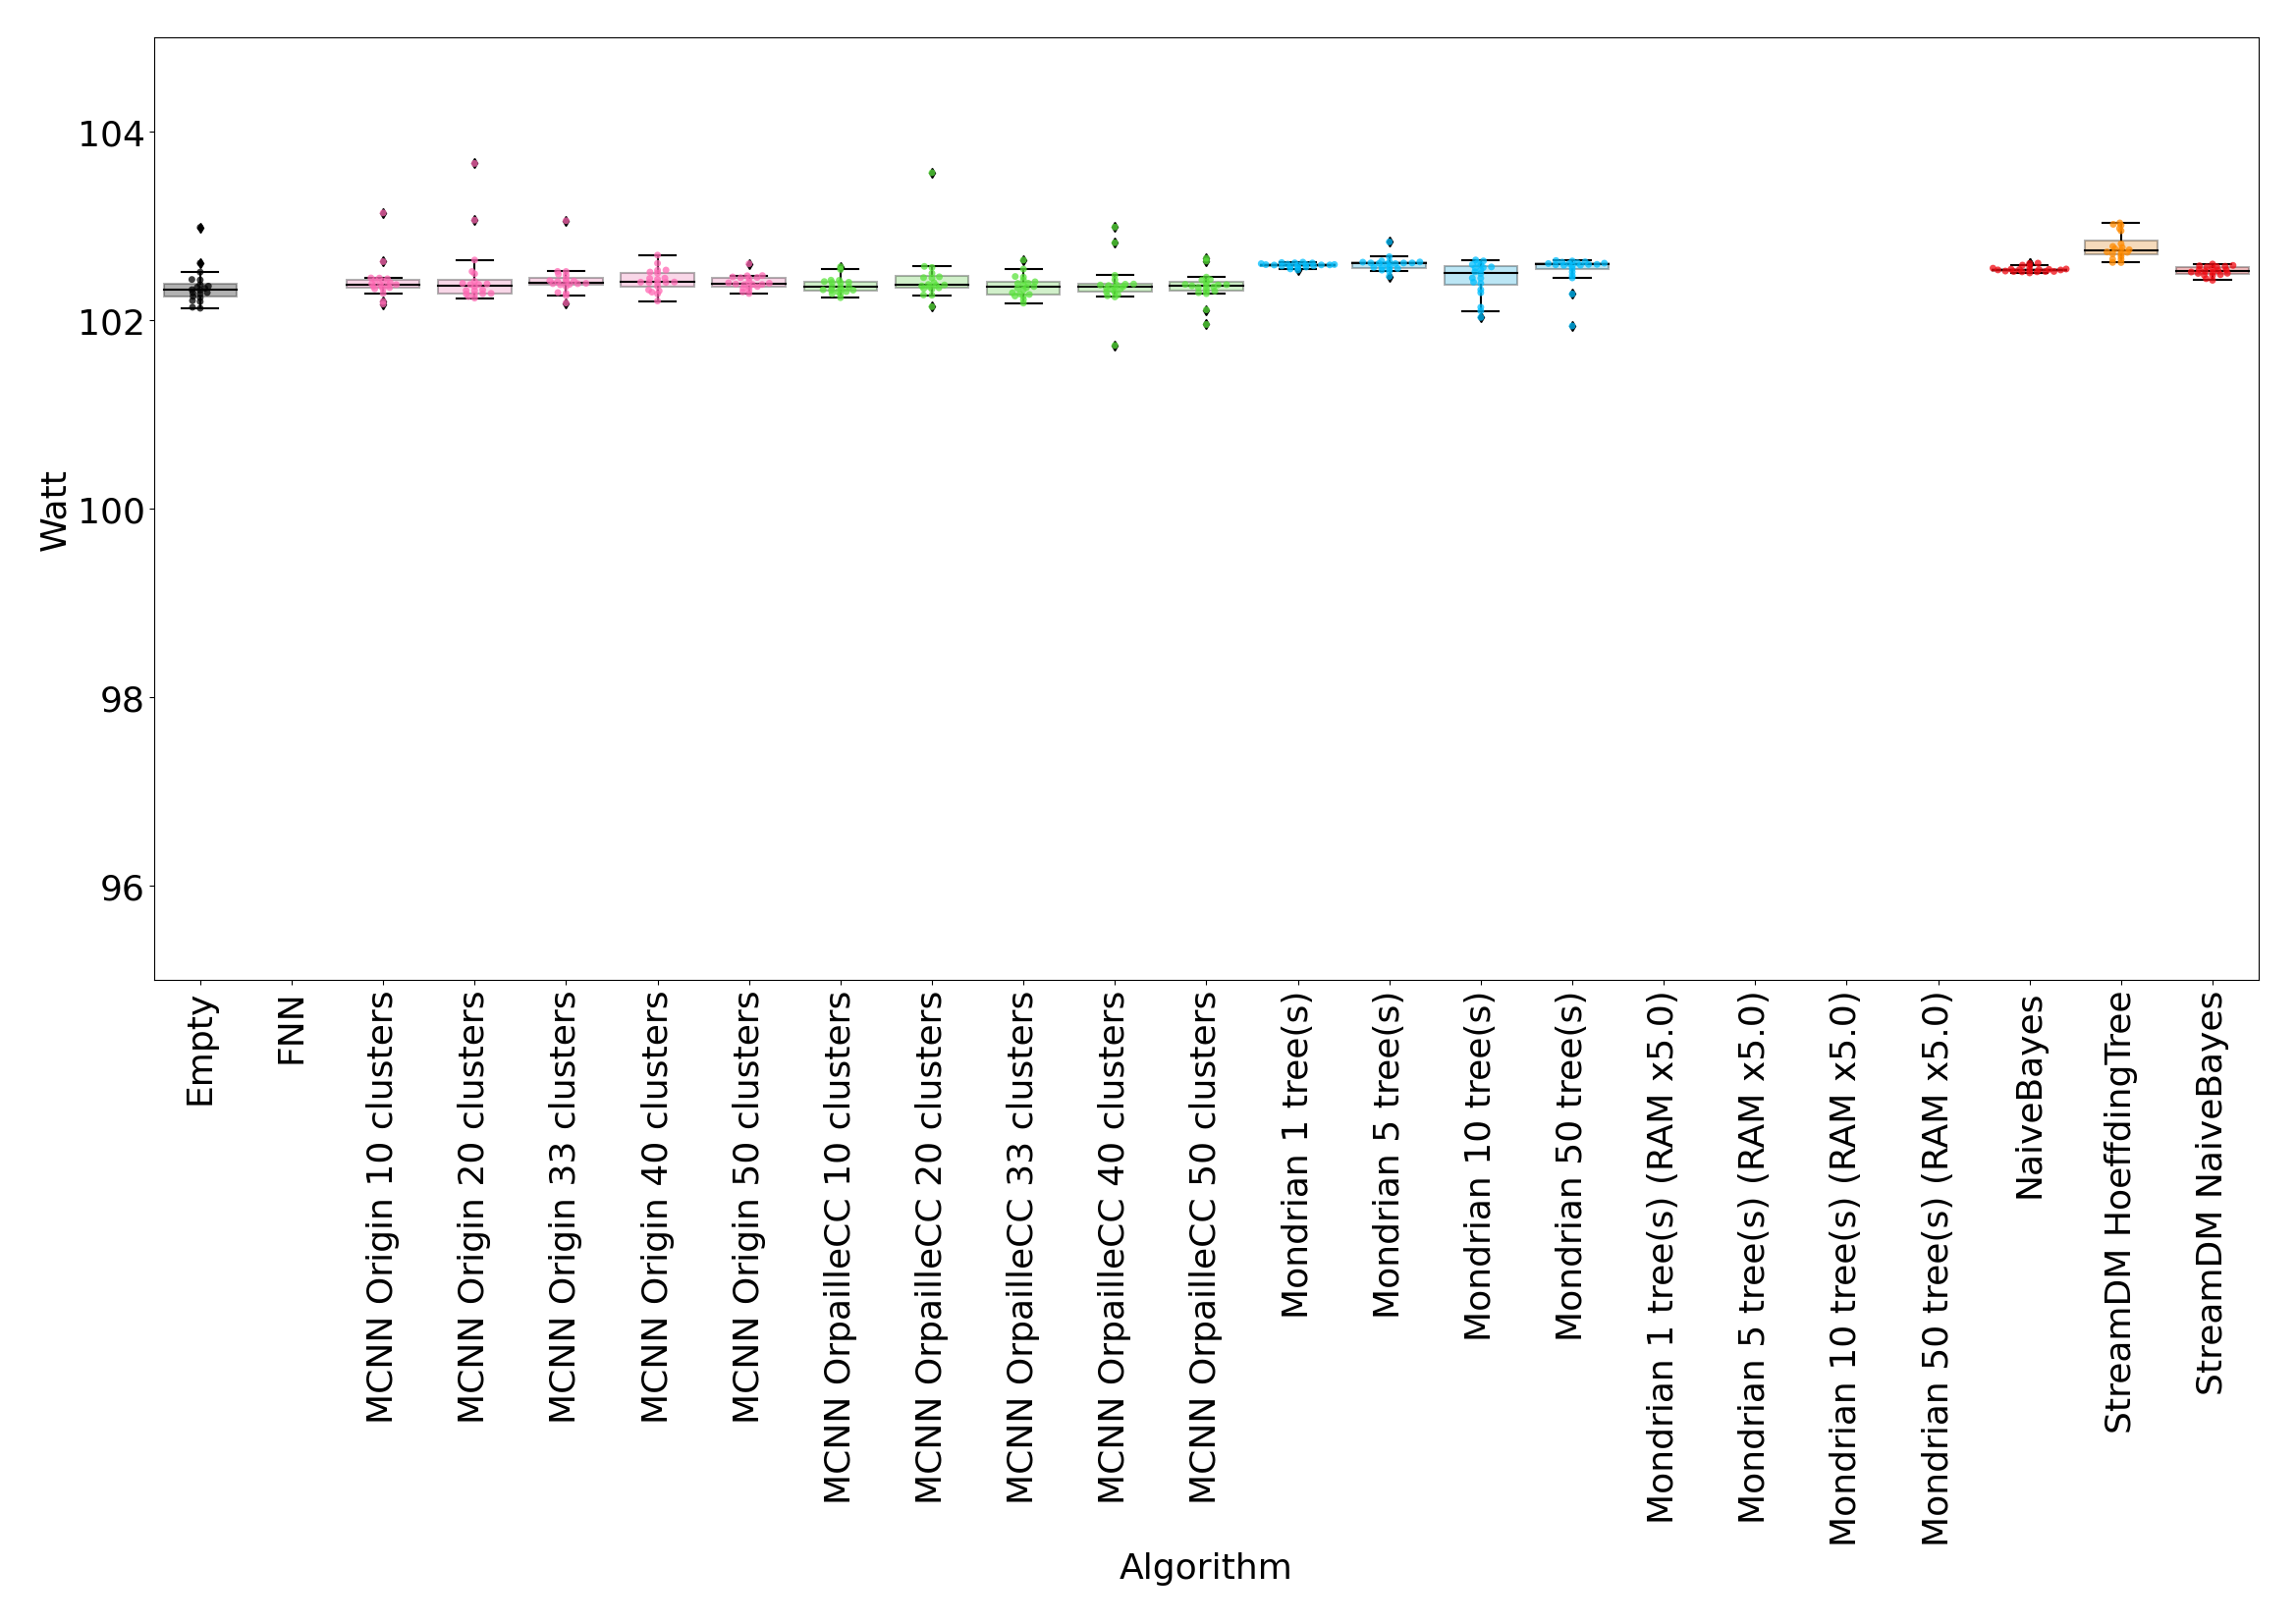
\includegraphics[width=\linewidth]{figures/results/recofit_3_watt.png}
		\caption{\recofitdataset}
		\label{fig:power-recofit}
	\end{subfigure}\\
	\begin{subfigure}[t]{.49\linewidth}
		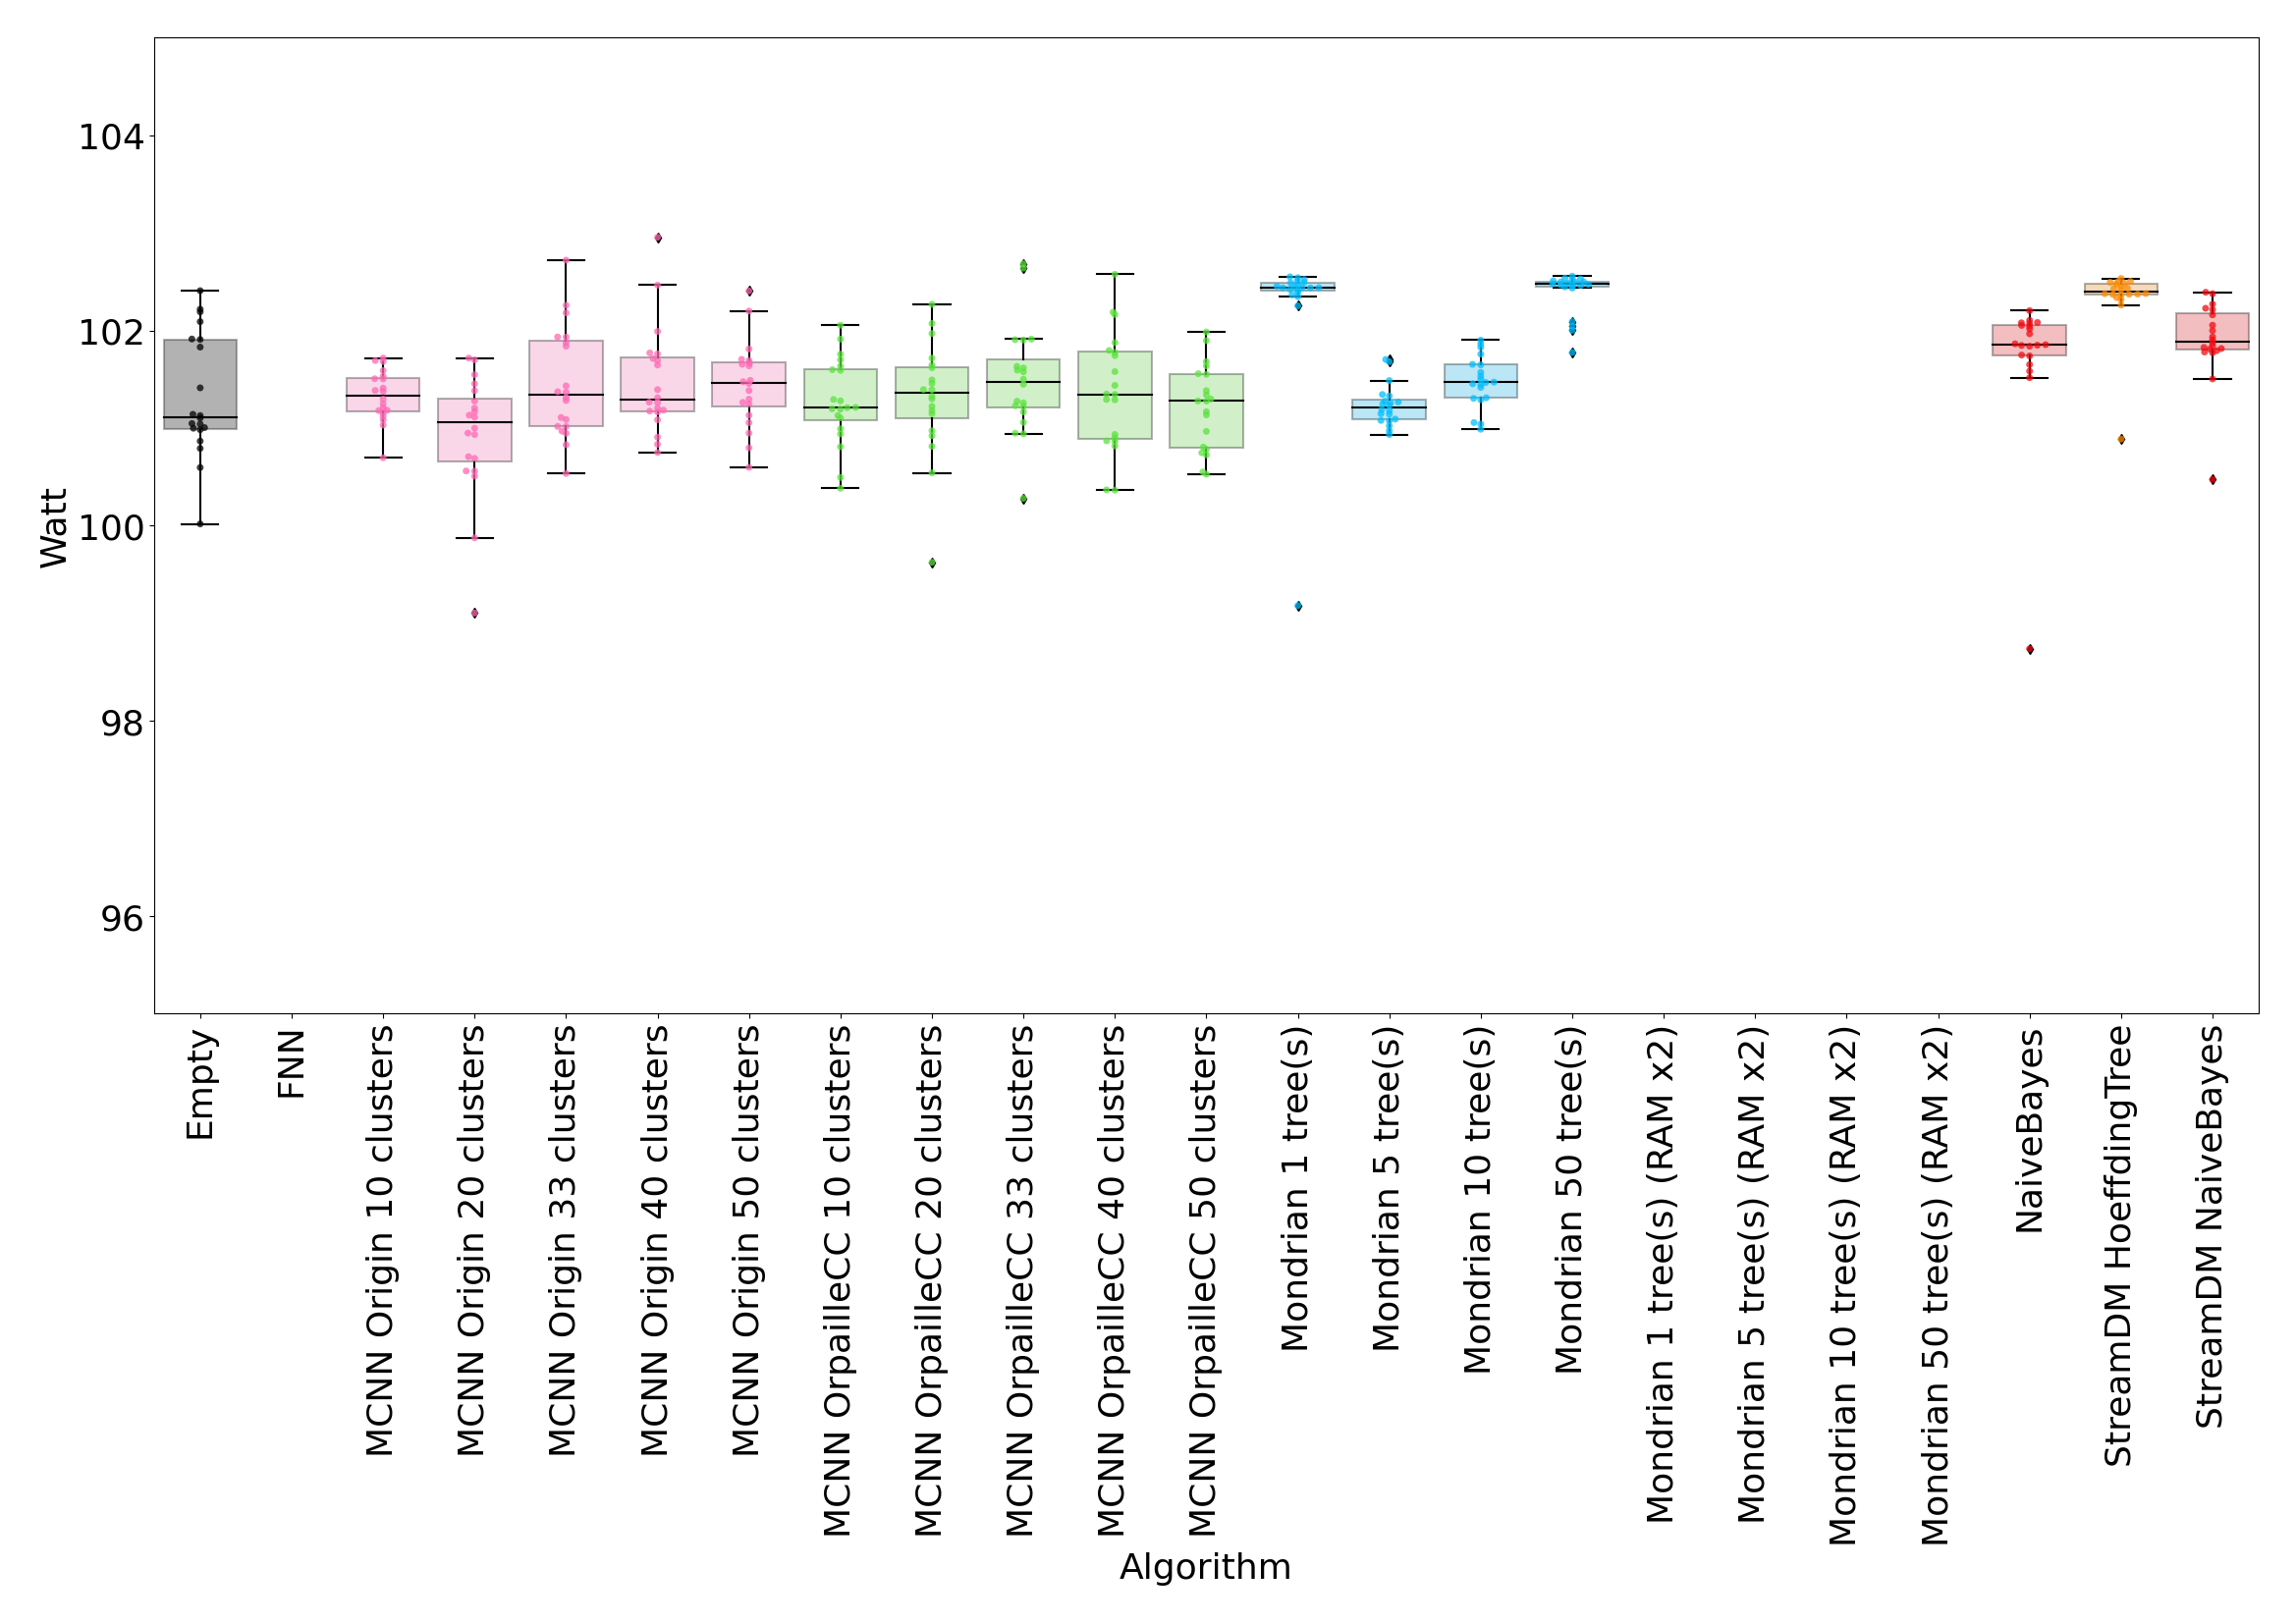
\includegraphics[width=\linewidth]{figures/results/drift_3_watt.png}
		\caption{\banosdataset with drift.}
		\label{fig:power-drift}
	\end{subfigure}
	\hfill
	\begin{subfigure}[t]{.49\linewidth}
		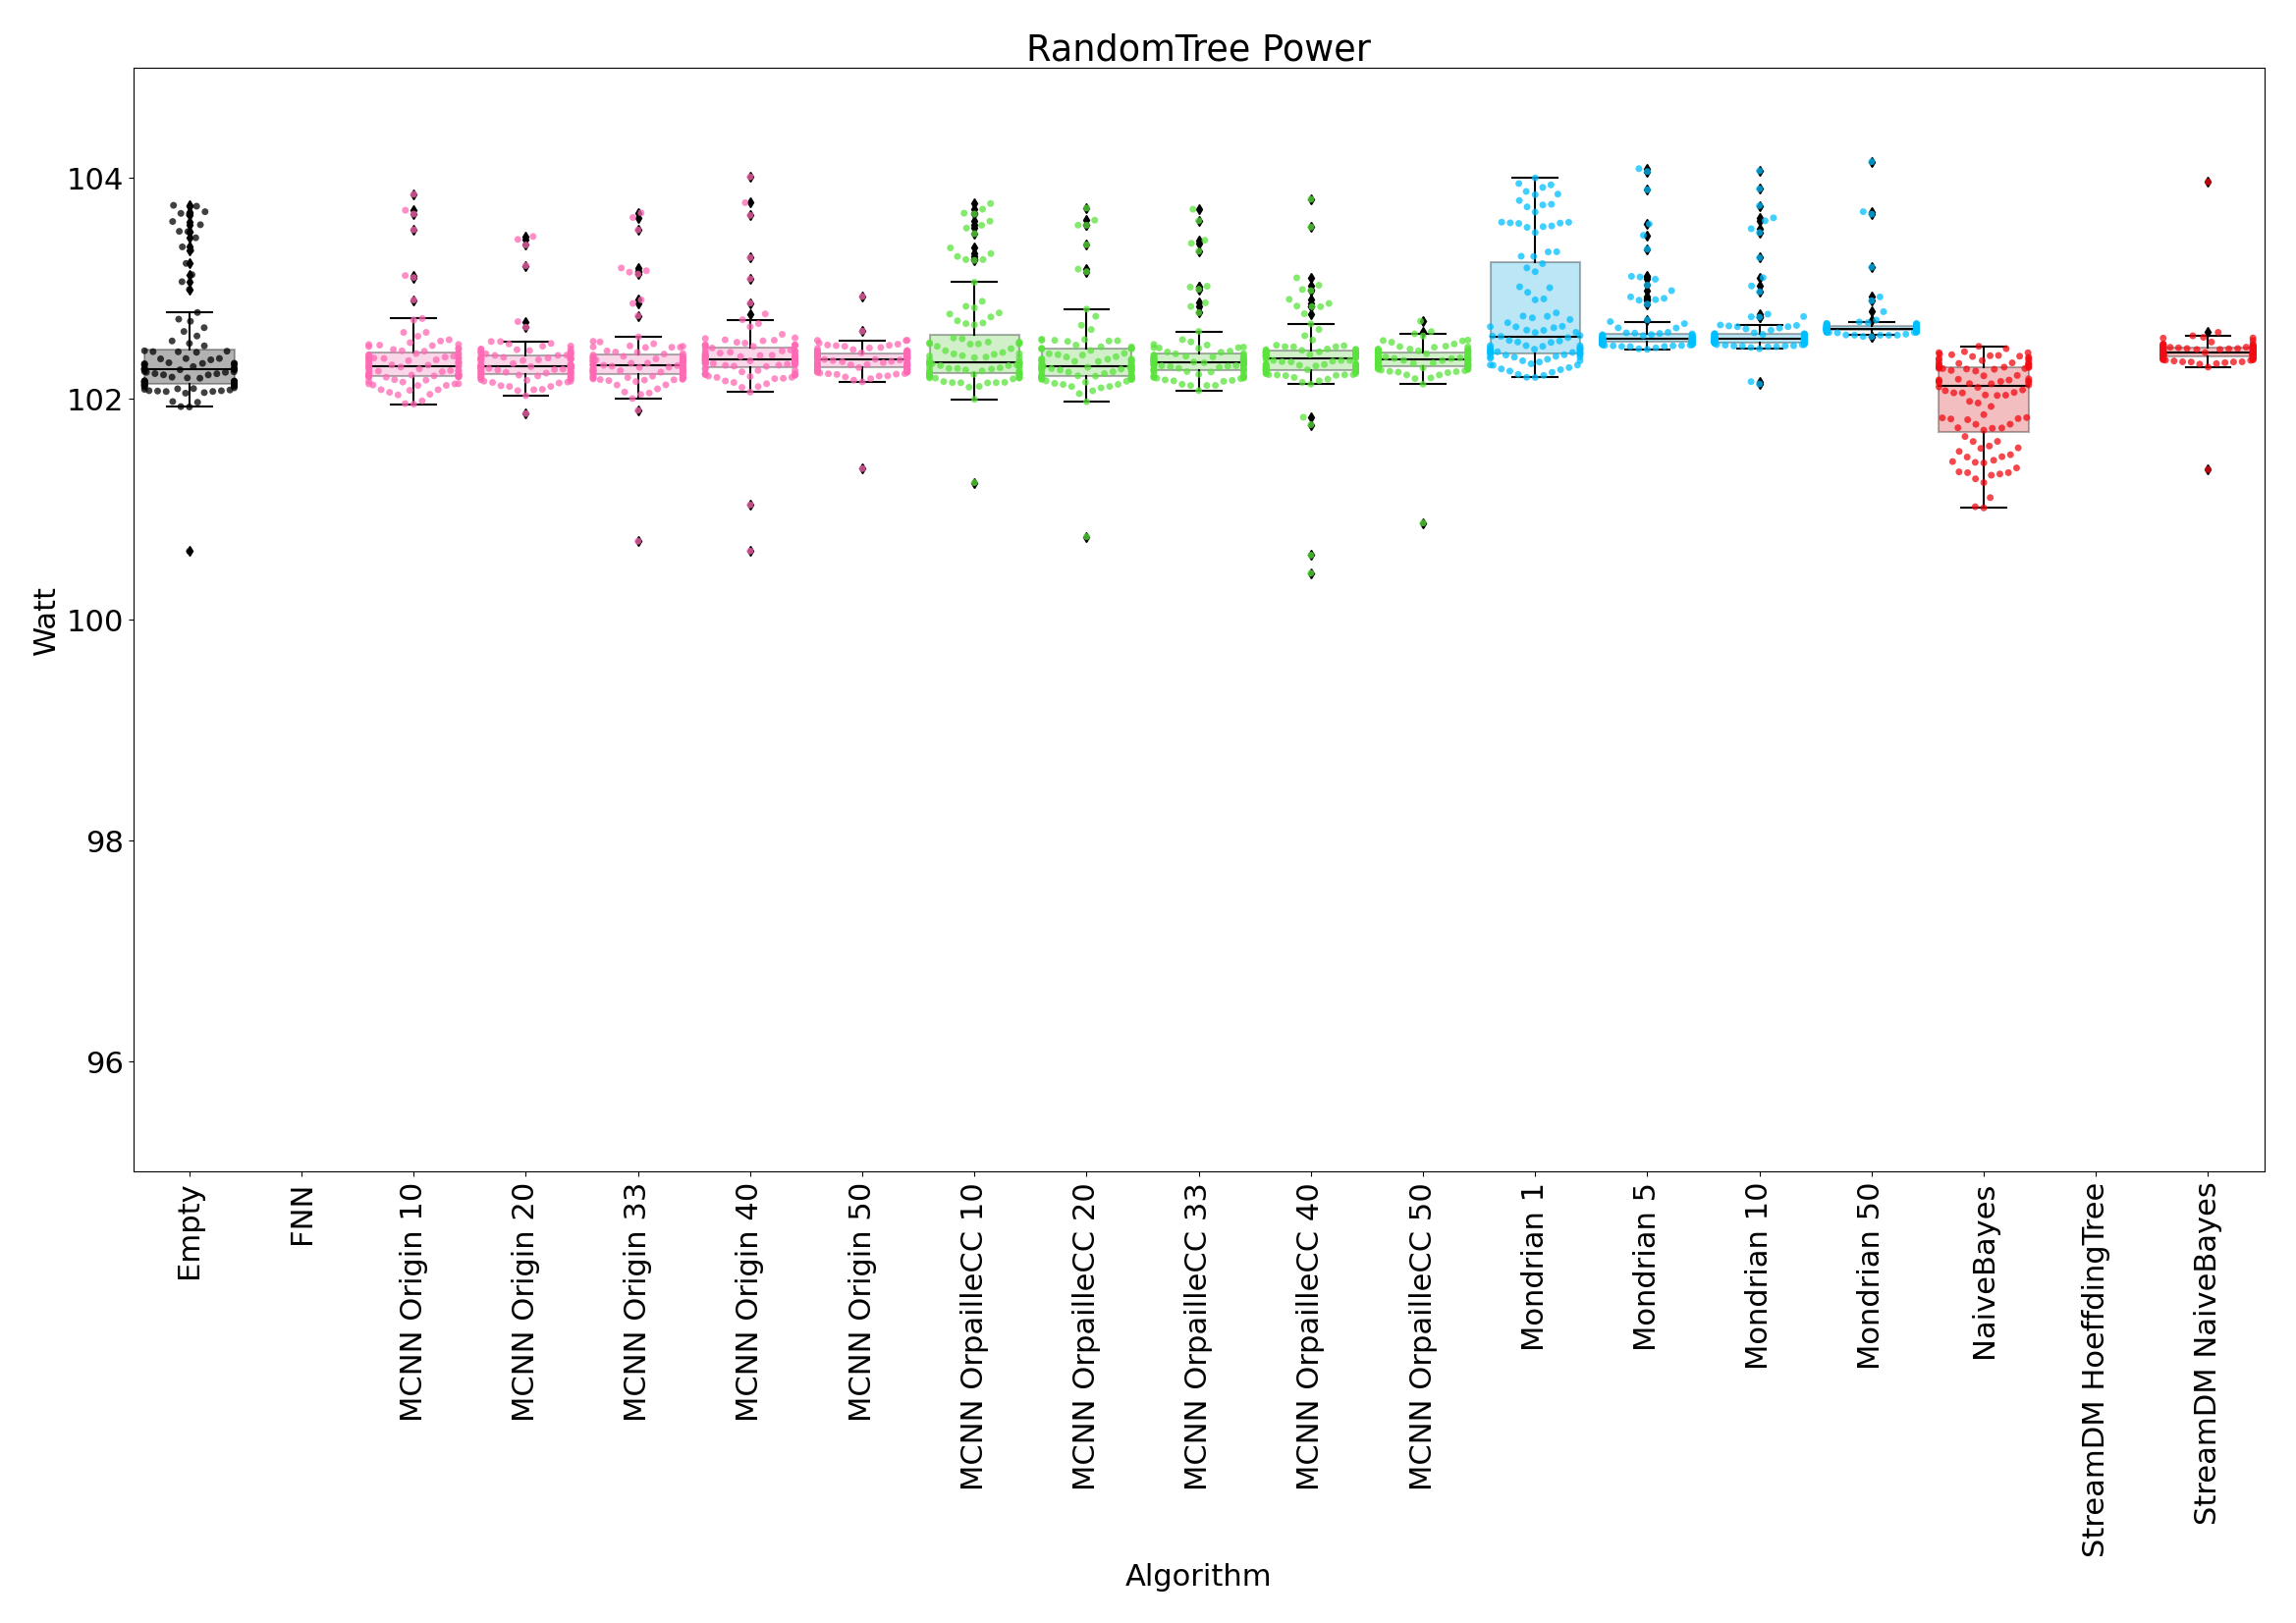
\includegraphics[width=\linewidth]{figures/results/dataset_3_watt.png}
		\caption{RandomTree}
		\label{fig:power-dataset_3}
	\end{subfigure}
	\caption{Power usage for four datasets.}
	\label{fig:power}
\end{figure*}
\subsection{Power}
\label{sec:result-power}
Figure~\ref{fig:power} shows the power usage of each classifier on four
datasets. Since all classifiers
exhibit comparable power consumptions, close to 102~W, we decided to show only
four of them.


\subsection{Runtime}
Figure~\ref{fig:runtime} shows the runtime of classifiers for the two real
datasets. The
\mondrianforest is the slowest classifier, in particular for 50 trees. The
second slowest classifier is the \hoeffdingtree, with a runtime comparable to the
\mondrianforest with 10 trees. The \hoeffdingtree is followed by the two \naivebayes
implementations, which is not surprising since \naivebayes classifiers are used
in the leaves of the \hoeffdingtree. The \mcnn classifiers are the fastest
ones, with a runtime very close to the empty classifier.

We observe that the runtime of StreamDM's \naivebayes is comparable to
 OrpailleCC's. This suggests that the performance of the two
 libraries is similar, which justifies our comparision of \hoeffdingtree
 and \mondrianforest.

\begin{figure*}
	\begin{subfigure}[t]{.49\linewidth}
		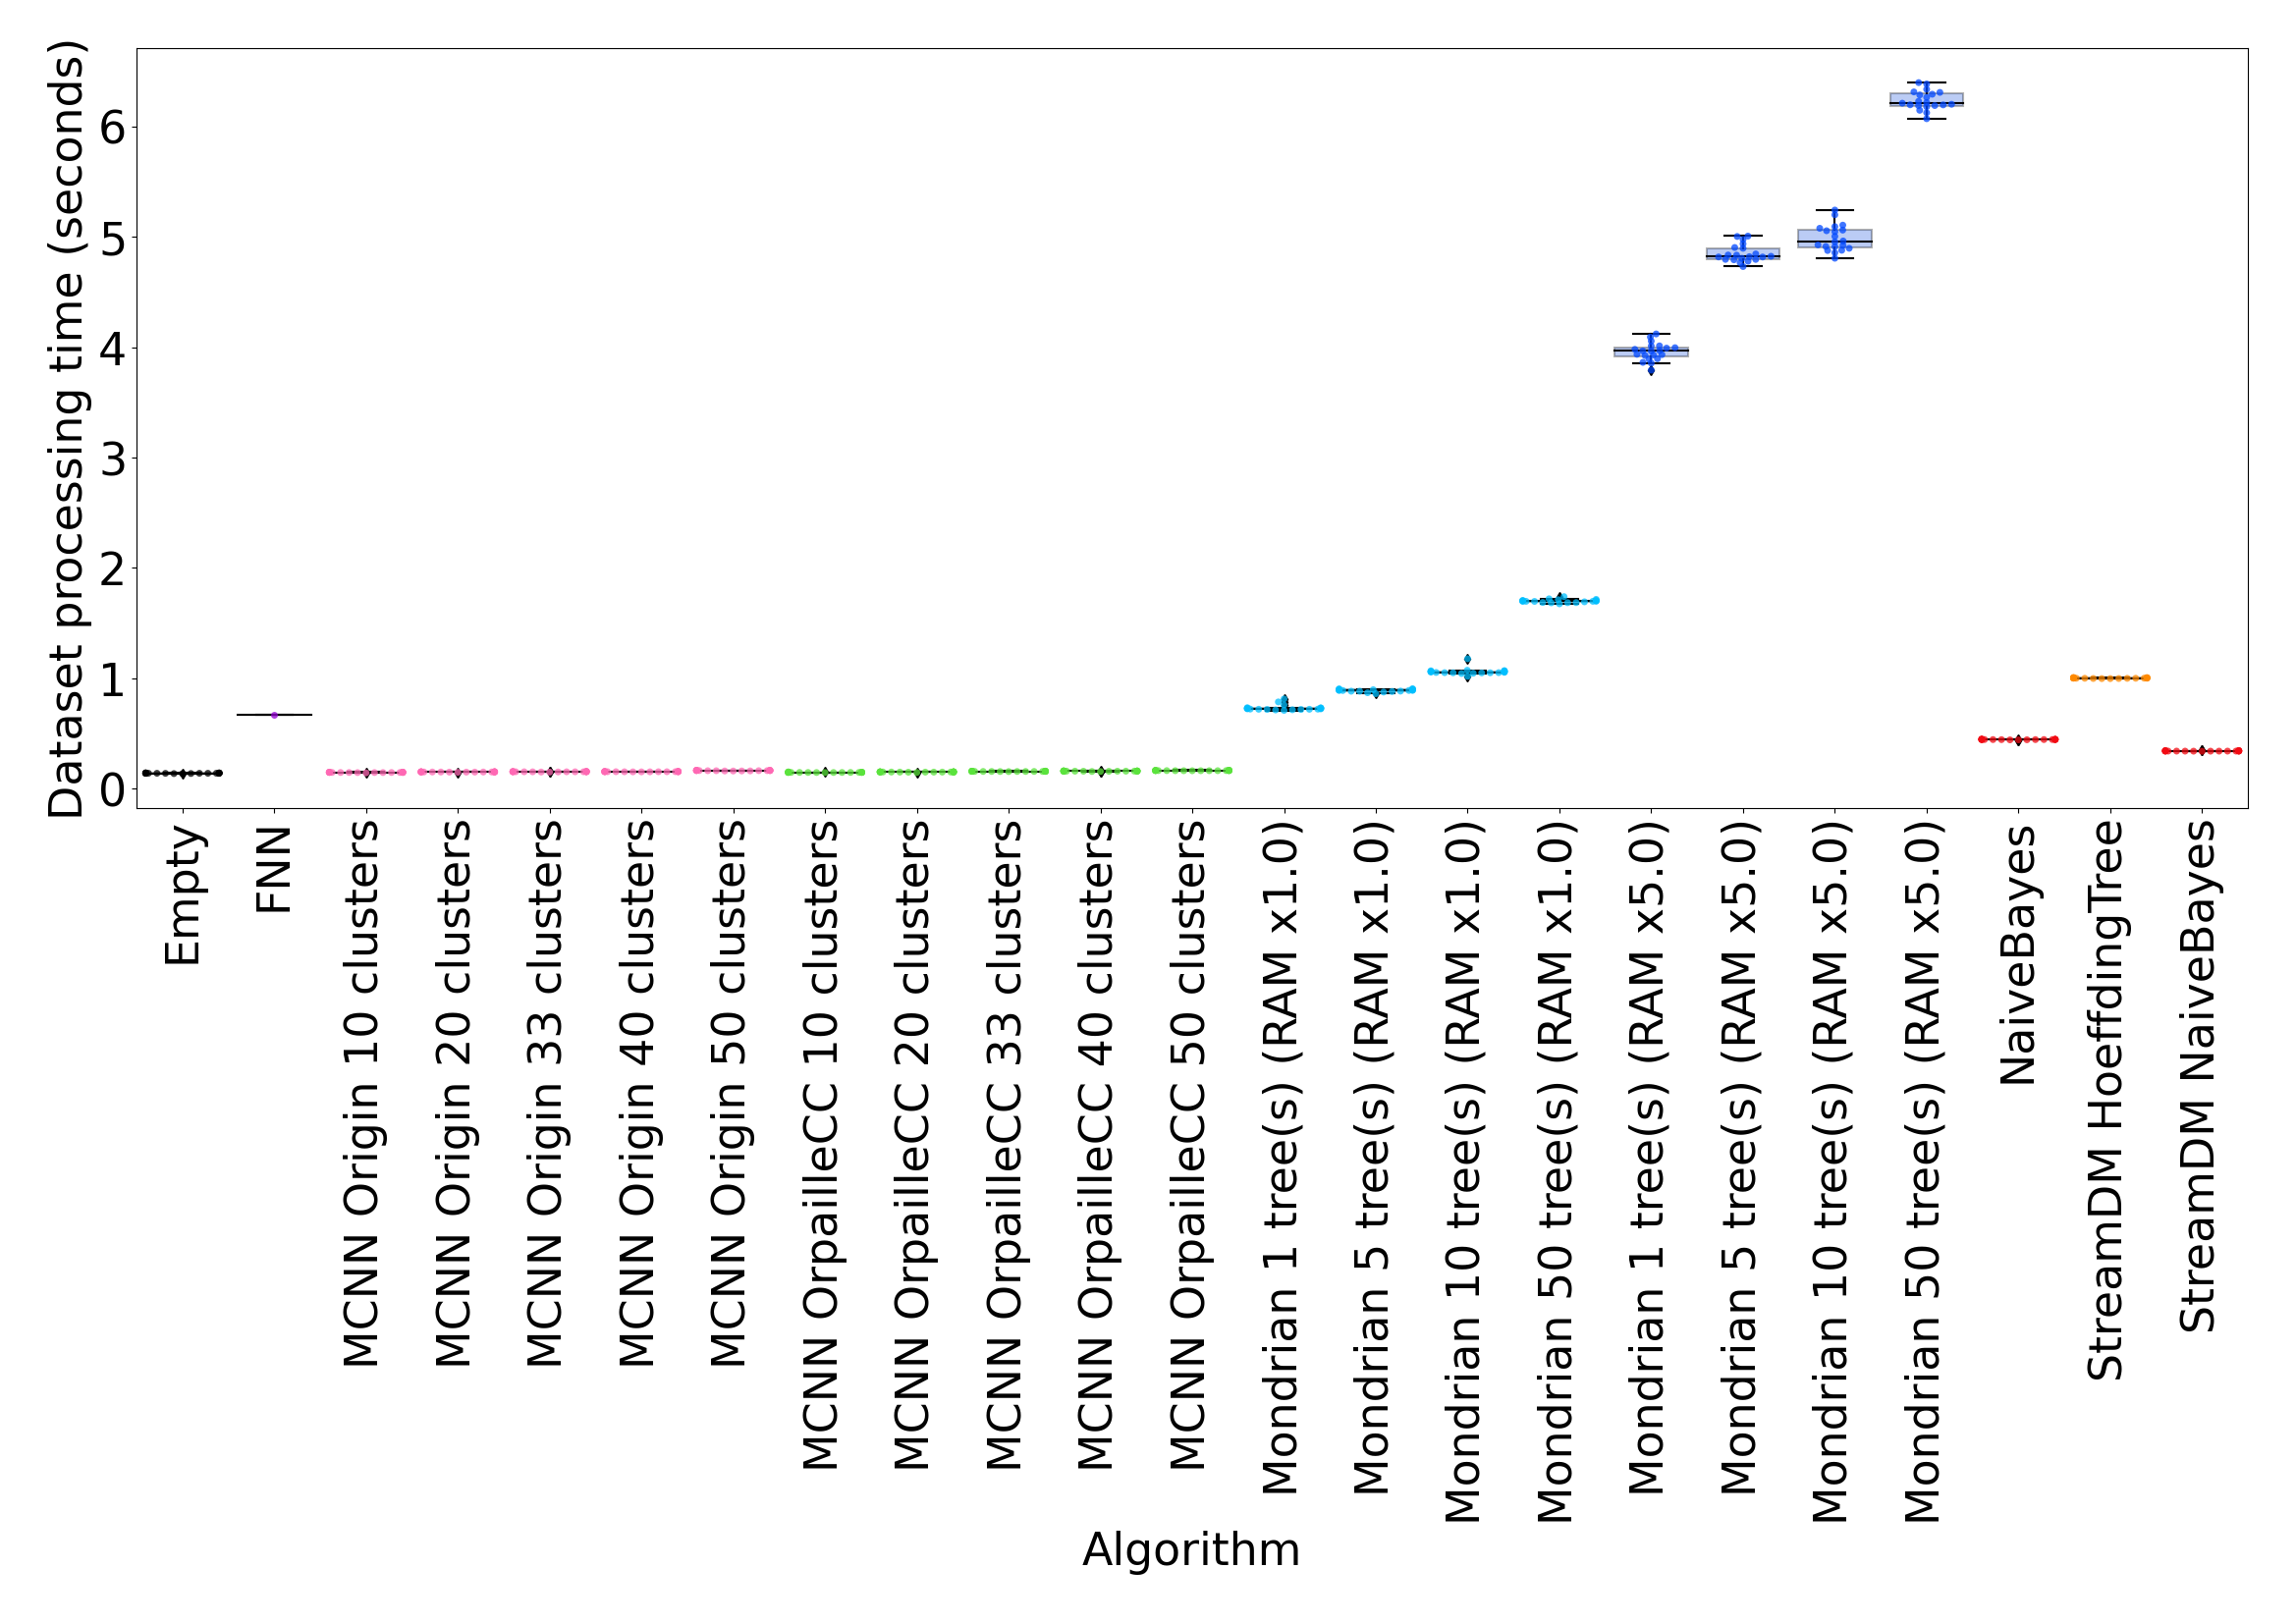
\includegraphics[width=\linewidth]{figures/results/banos_6_runtime.png}
		\caption{\banosdataset}
		\label{fig:runtime-banos}
	\end{subfigure}
	\hfill
	\begin{subfigure}[t]{.49\linewidth}
		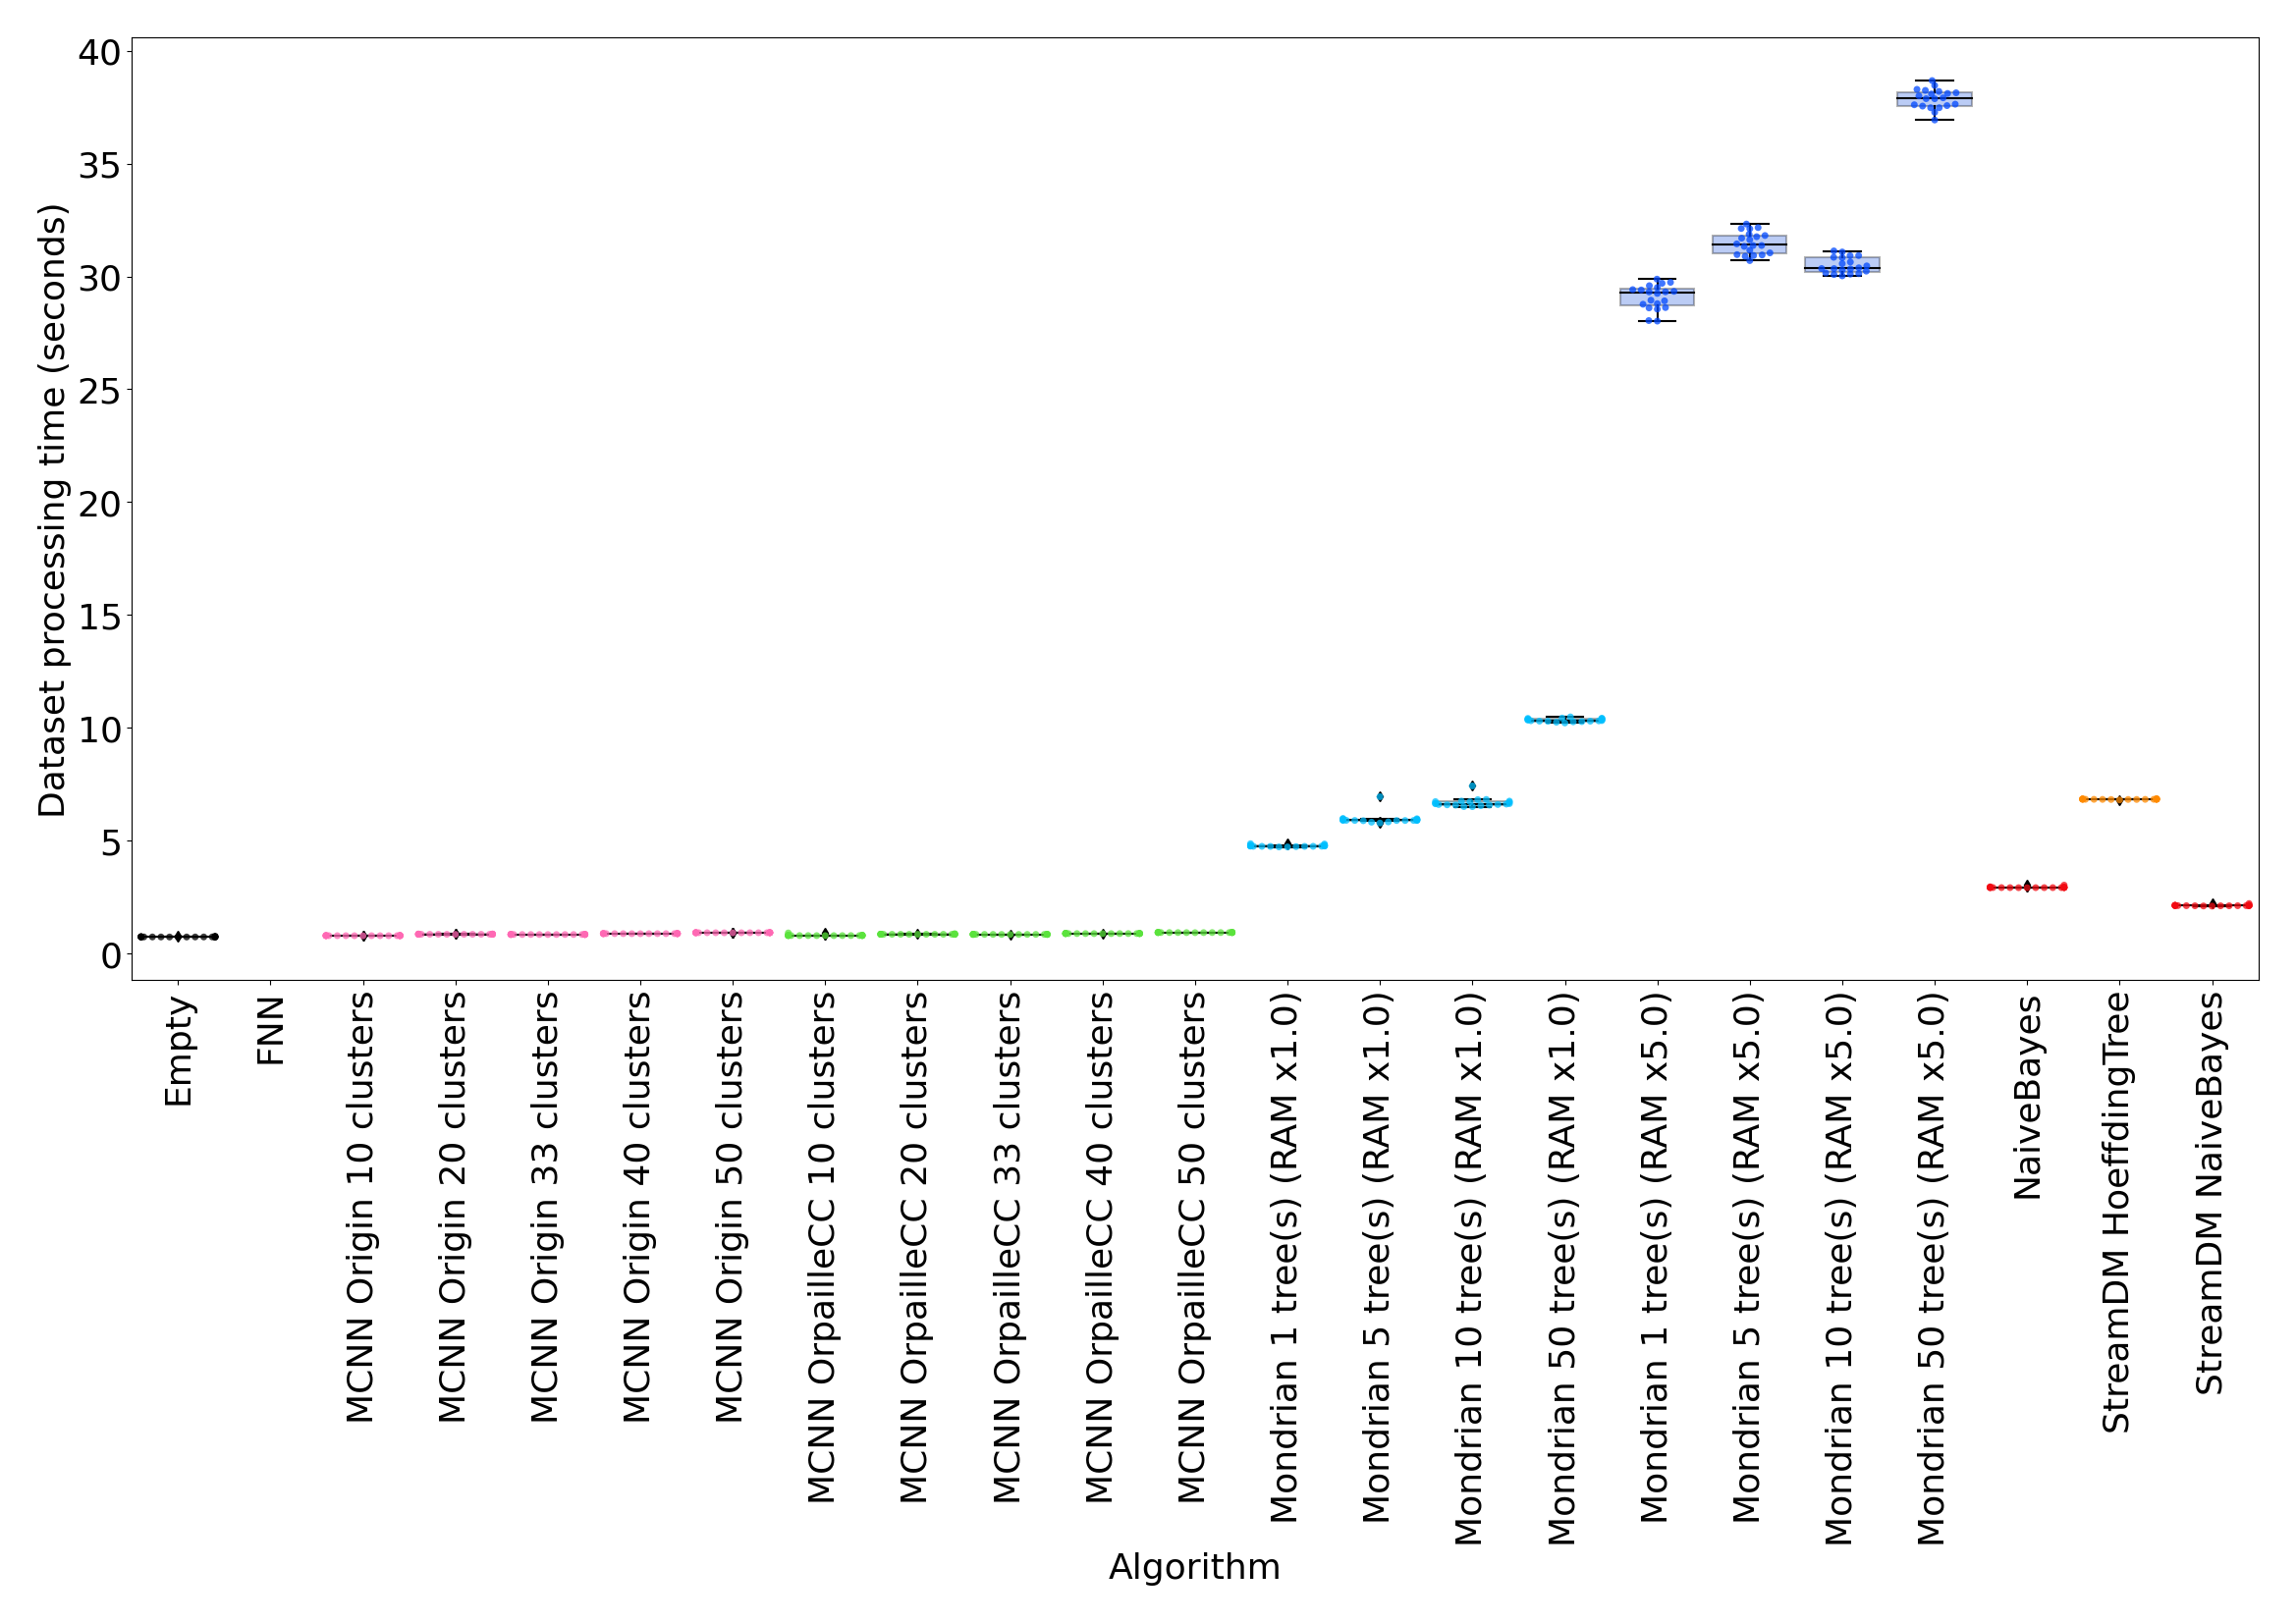
\includegraphics[width=\linewidth]{figures/results/recofit_6_runtime.png}
		\caption{\recofitdataset}
		\label{fig:runtime-recofit}
	\end{subfigure}
	\caption{Runtime with the two real datasets (20 repetitions).}
	\label{fig:runtime}
\end{figure*}

\subsection{Memory}
\label{sec:result-memory}
Figure~\ref{fig:memory} shows the evolution of the memory footprint for the
\banosdataset dataset. Because we focus on the classifiers footprint, the
figure only shows the memory difference between the classifiers and the empty
classifier. 

Memory footprint is similar across all datasets \TG{do you mean across all classifiers?}, due to the fact that most
algorithms follow a bounded memory policy or have a constant space complexity.
The only exception is the \hoeffdingtree that constantly selects new splits
depending on new data points. The \mondrianforest has the same behavior but the
OrpailleCC implementation includes a memory bound, which makes its memory
footprint constant.

\TG{it looks like the hoeffding tree consumes way more memory, but isnt it a
side effect of using streamDM? Maybe all memory consumptions should be computed by reference 
to the naive bayes baseline. }

\begin{figure}
	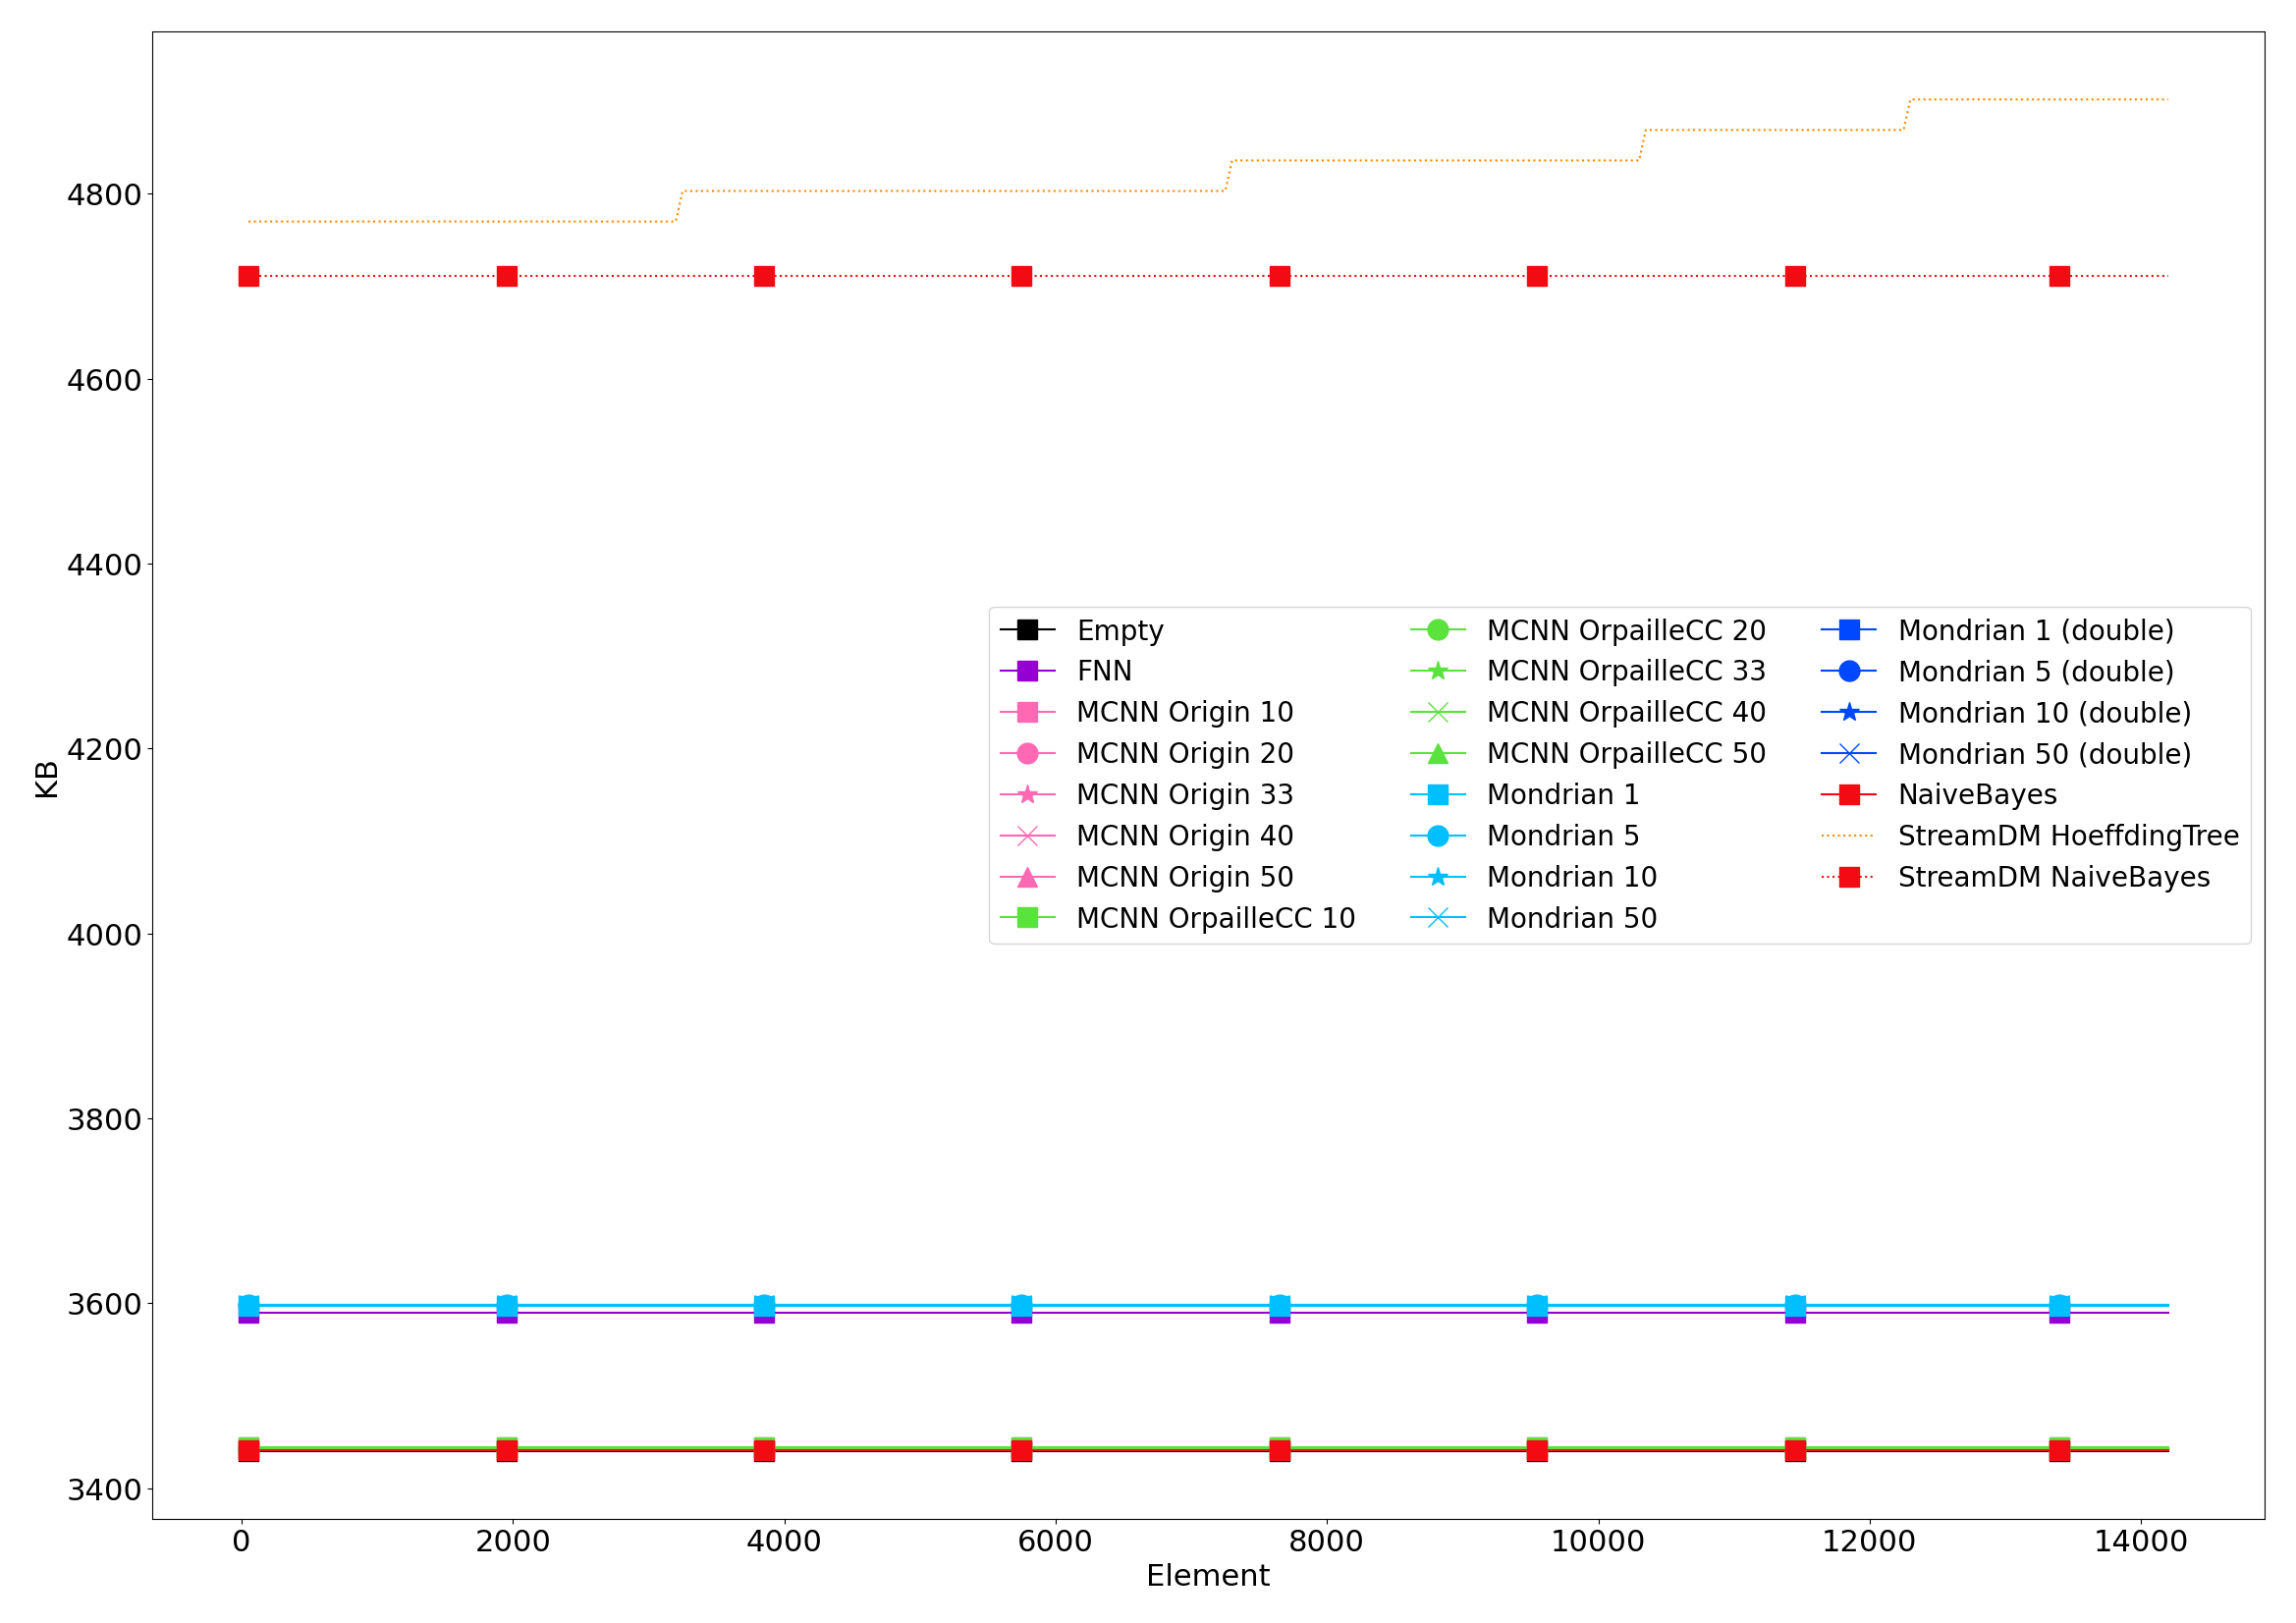
\includegraphics[width=\linewidth]{figures/results/banos_3_memory.png}
	\caption{Memory footprint of the classifiers relatively to the empty
	classifier, measured on the \banosdataset dataset. The memory footprint of the empty
	classifier is slightly above 3.4~MB \TG{give the exact value}.}
	\label{fig:memory}
\end{figure}


\subsection{Micro-Cluster Nearest Neighbor Hyperparameters}

Figure~\ref{fig:mcnn-tuning-error} shows the impact of the error threshold
in the \mcnn classifiers with different cluster counts \TG{write ``error threshold'' in the figure legend}. The error
threshold of \mcnn has little impact on the classification performance. For
20 and 40 clusters, the best-performing threshold is either 2 or 4, meaning
that a cluster may do 2 or 4 errors before being split. For 10 clusters,
all error thresholds perform equally.

\begin{figure}
	 \begin{subfigure}[b]{0.49\textwidth}
		 \centering
		 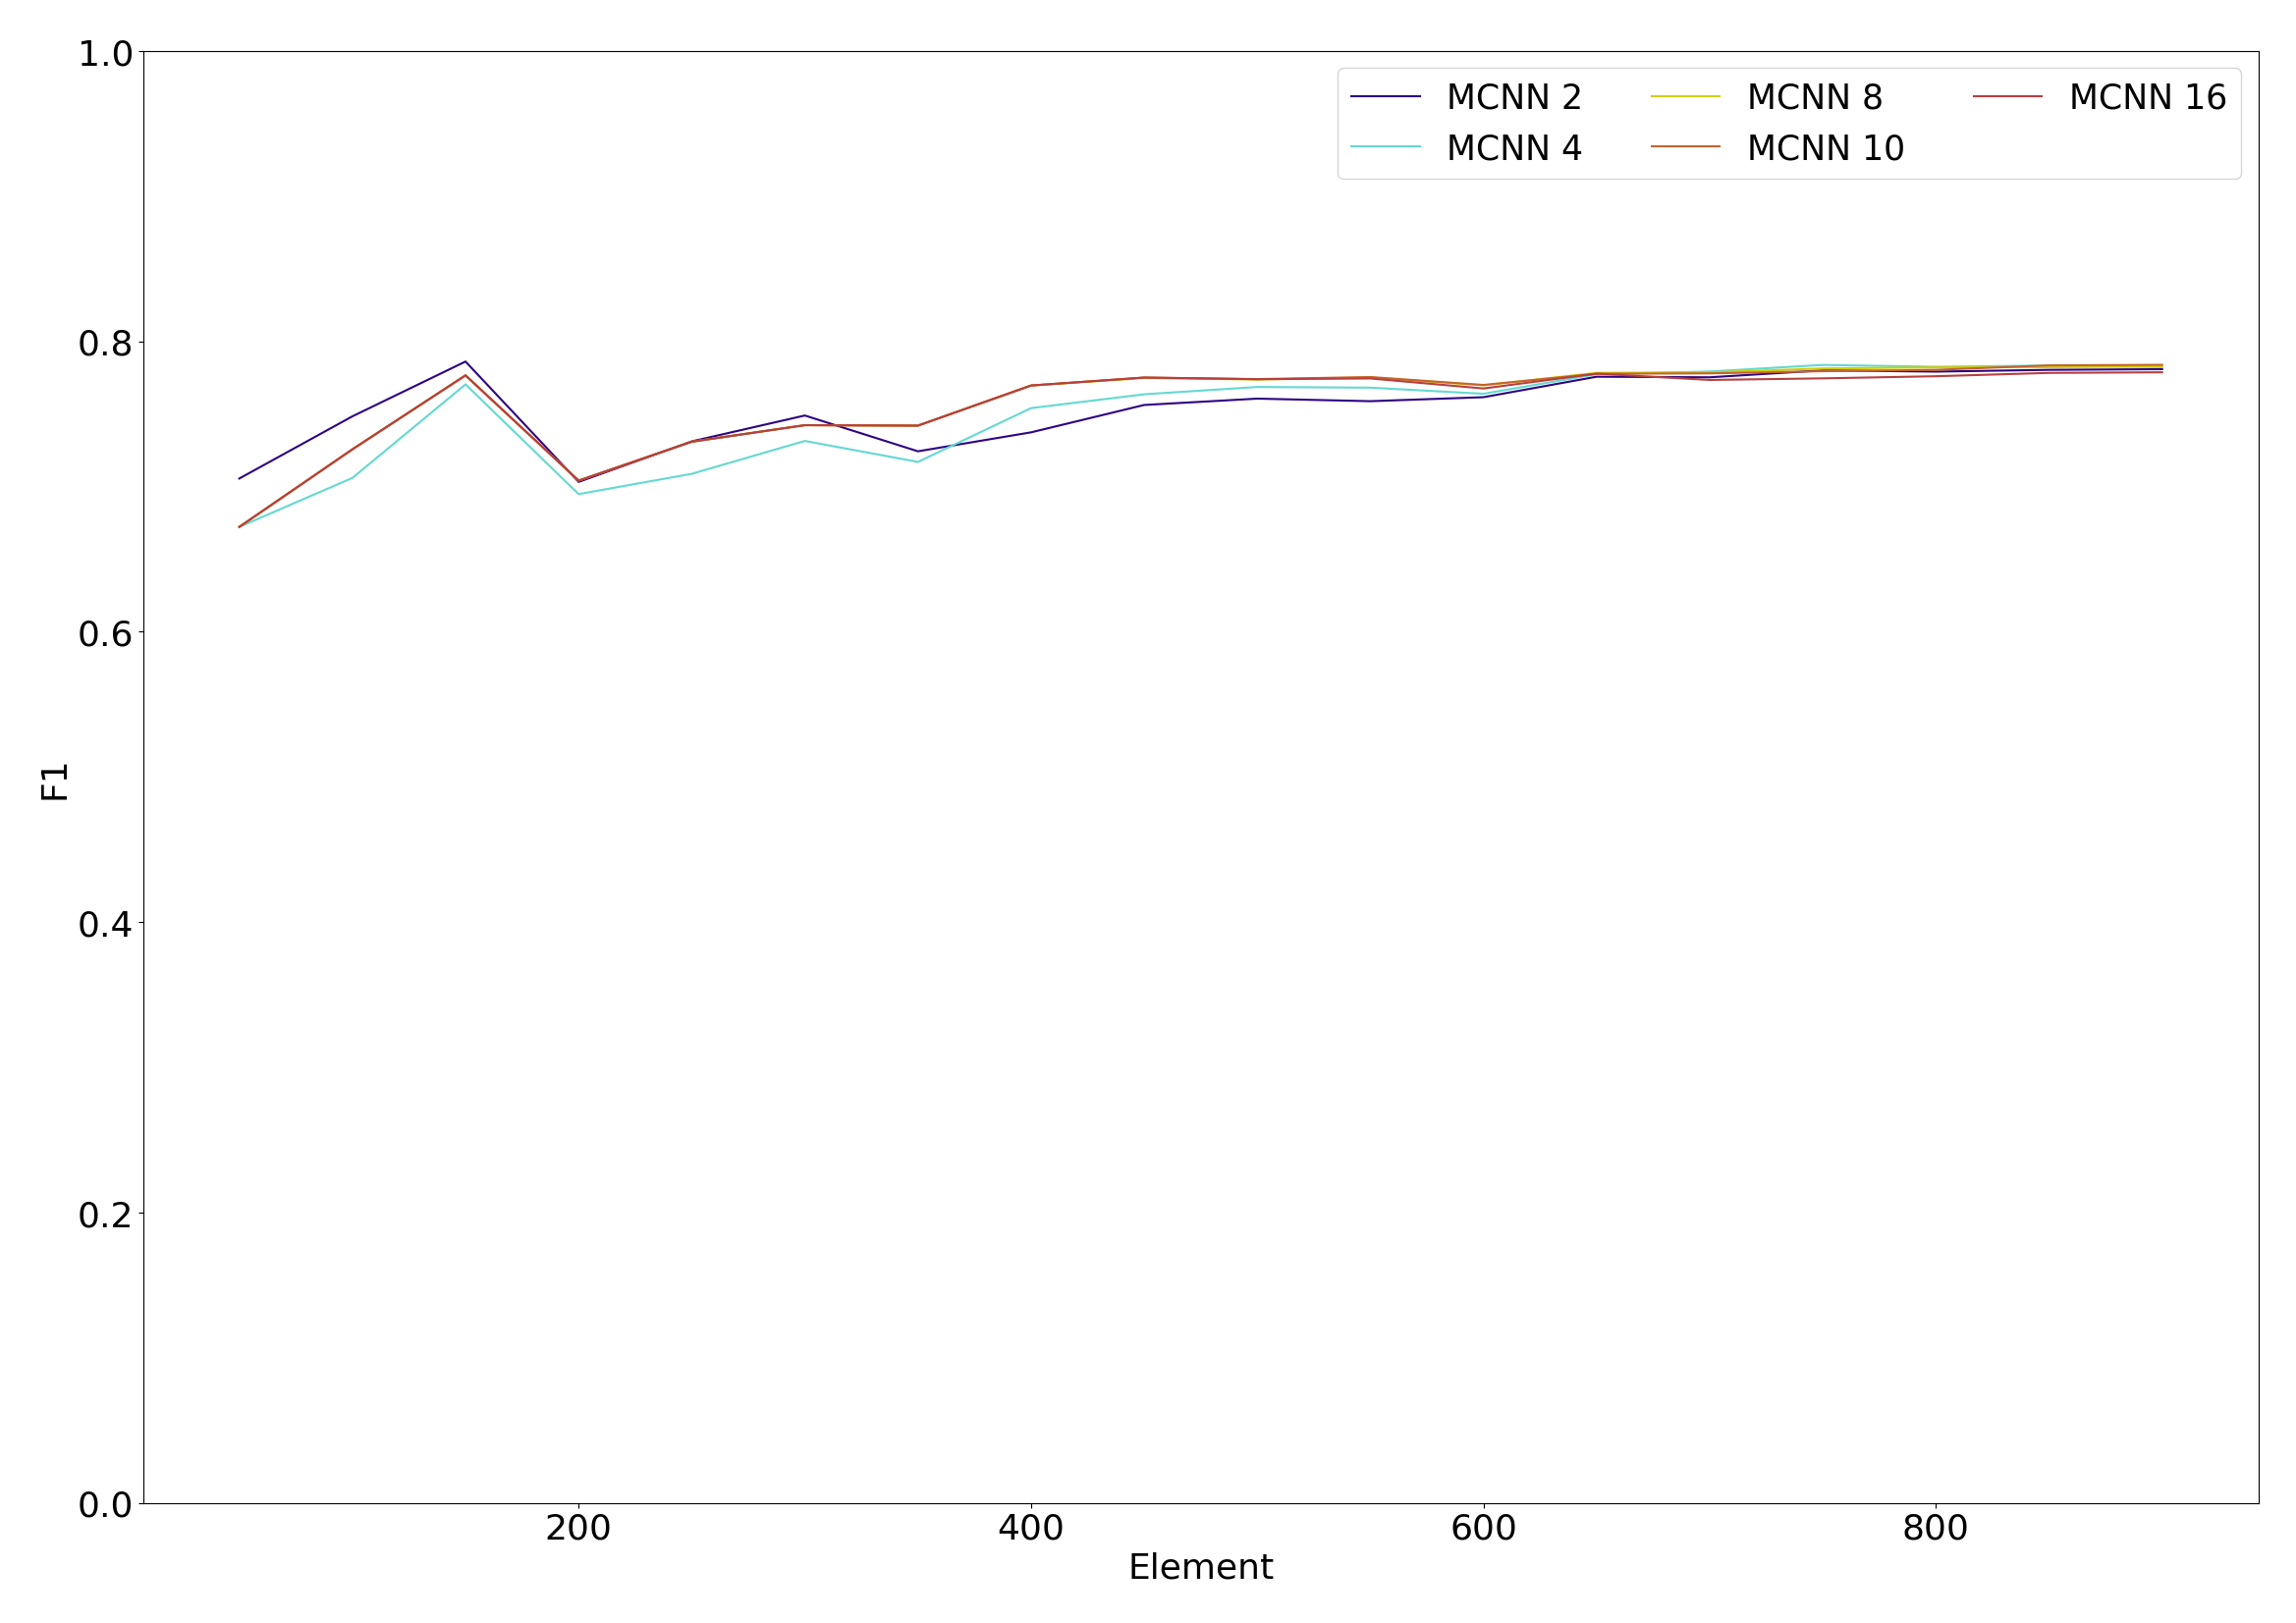
\includegraphics[width=\linewidth]{figures/calibration_mcnn_40.png}
		 \caption{40 clusters}
	 \end{subfigure}
	 \begin{subfigure}[b]{0.49\textwidth}
		 \centering
		 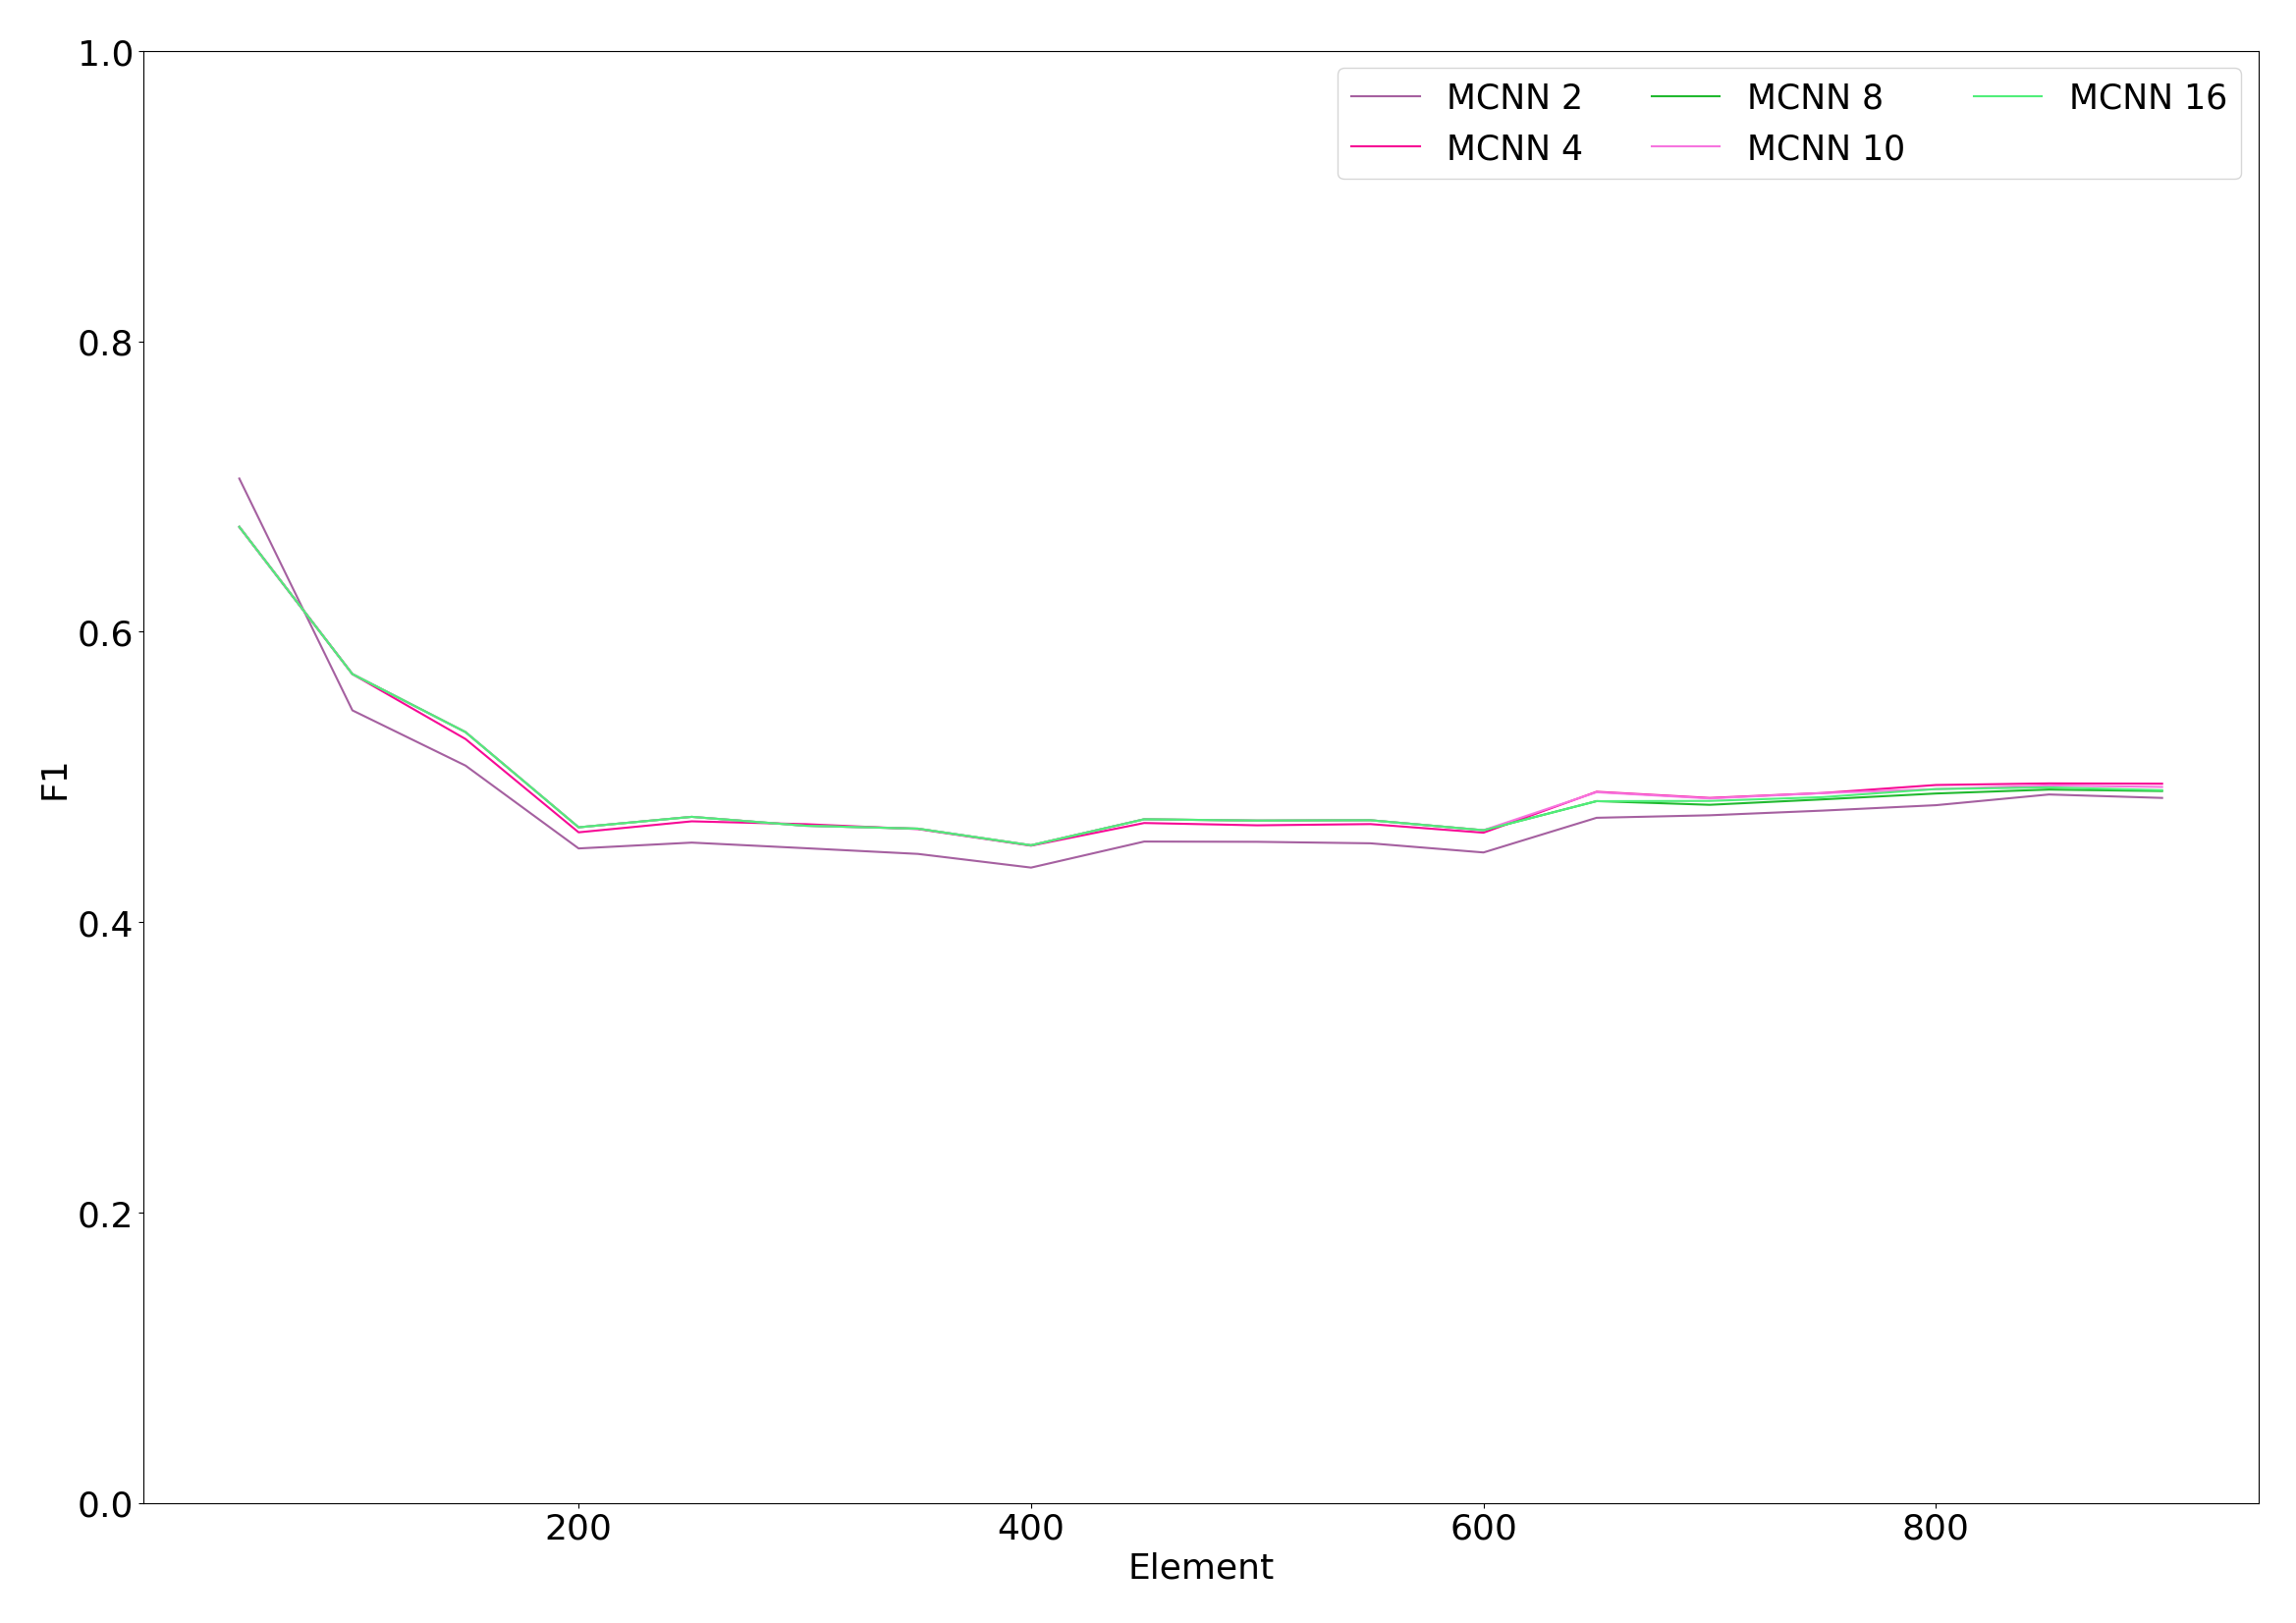
\includegraphics[width=\linewidth]{figures/calibration_mcnn_20.png}
		 \caption{20 clusters}
	 \end{subfigure}
	 \begin{subfigure}[b]{0.49\textwidth}
		 \centering
		 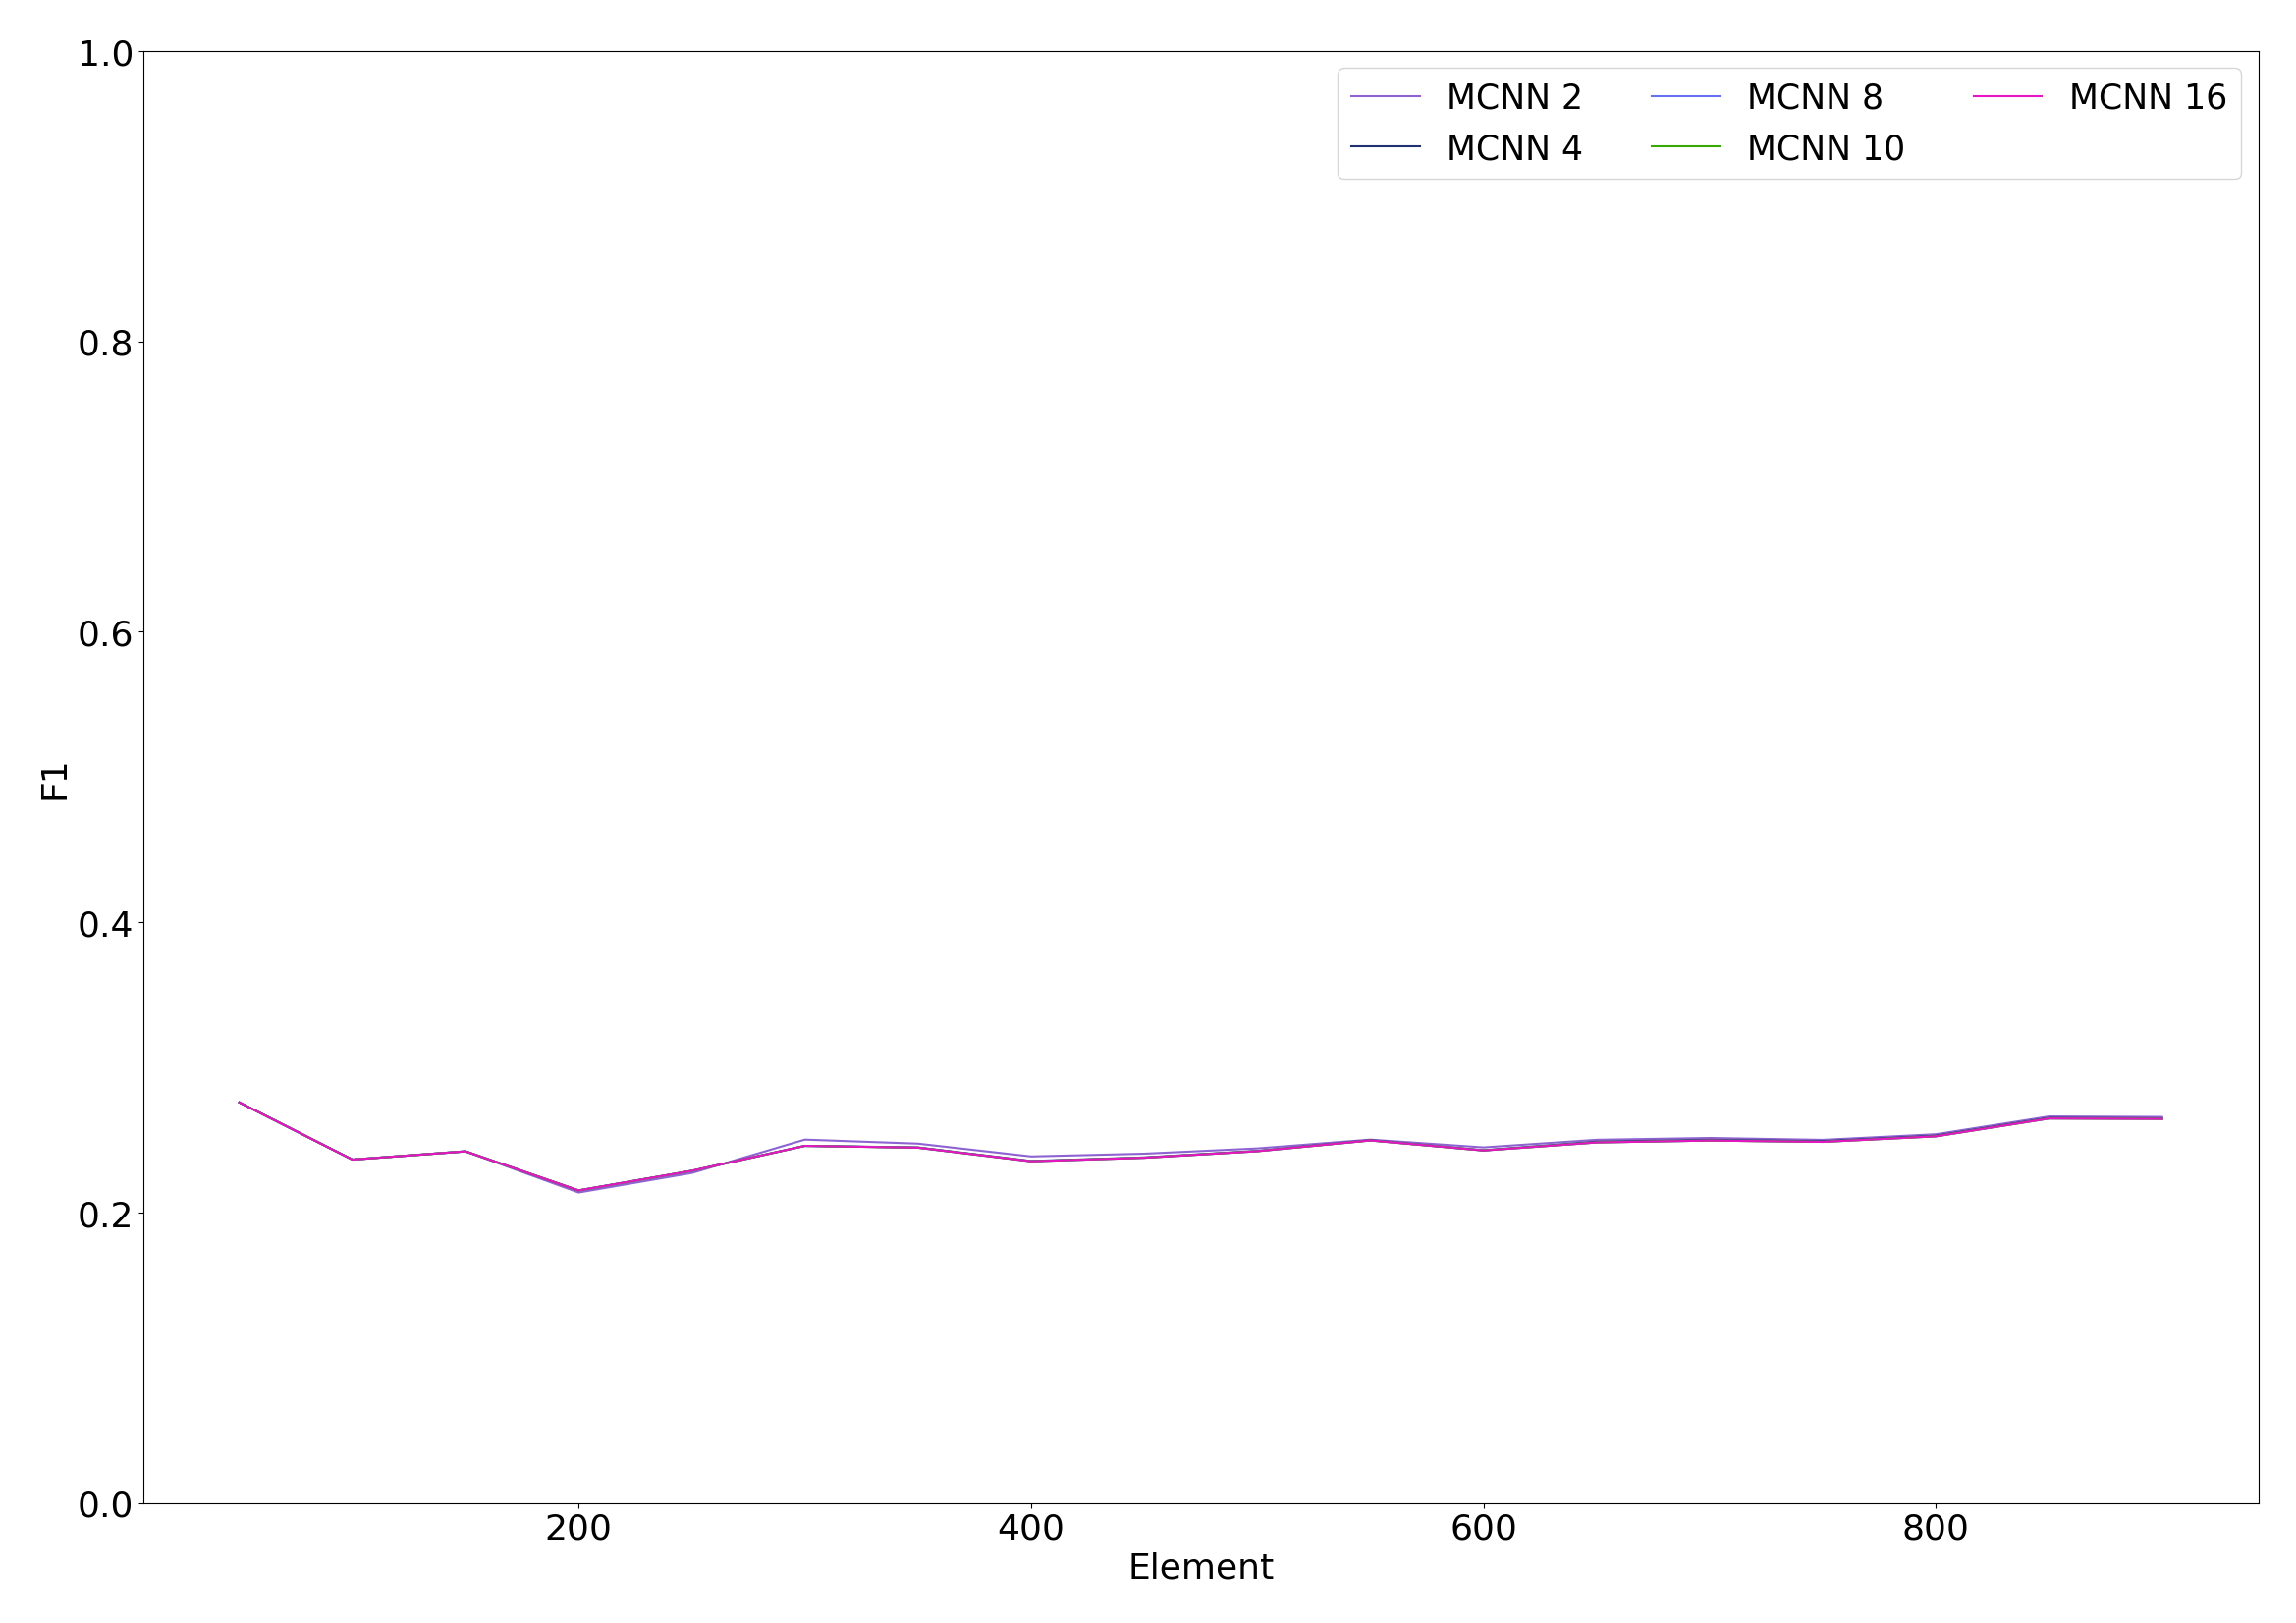
\includegraphics[width=\linewidth]{figures/calibration_mcnn_10.png}
		 \caption{10 clusters}
	 \end{subfigure}
	\caption{Hyperparameters tuning of \mcnn with first subject of \banosdataset dataset.}
	\label{fig:mcnn-tuning-error}
\end{figure}

\subsection{\mondrianforest Hyperparameters}

Figure~\ref{fig:mondrian-tuning} shows the impact of the \mondrianforest hyperparameters on
the classification performance. 

The base count hyperparameter (Figure~\ref{fig:mondrian-base-count}) has a
very substantial impact on classification performance; the smallest value
(0.0) results in the best performance. On the contrary, the
budget hyperparameter (Figure~\ref{fig:mondrian-budget}) only has a
moderate impact on classification; the best value is 0.2. Finally, the discount hyperparameter
(Figure~\ref{fig:mondrian-discount}) has a negligible impact on the
performance; the best-performing value is 0.1.

\begin{figure}
	 \centering
	 \begin{subfigure}[b]{0.49\textwidth}
		\centering
		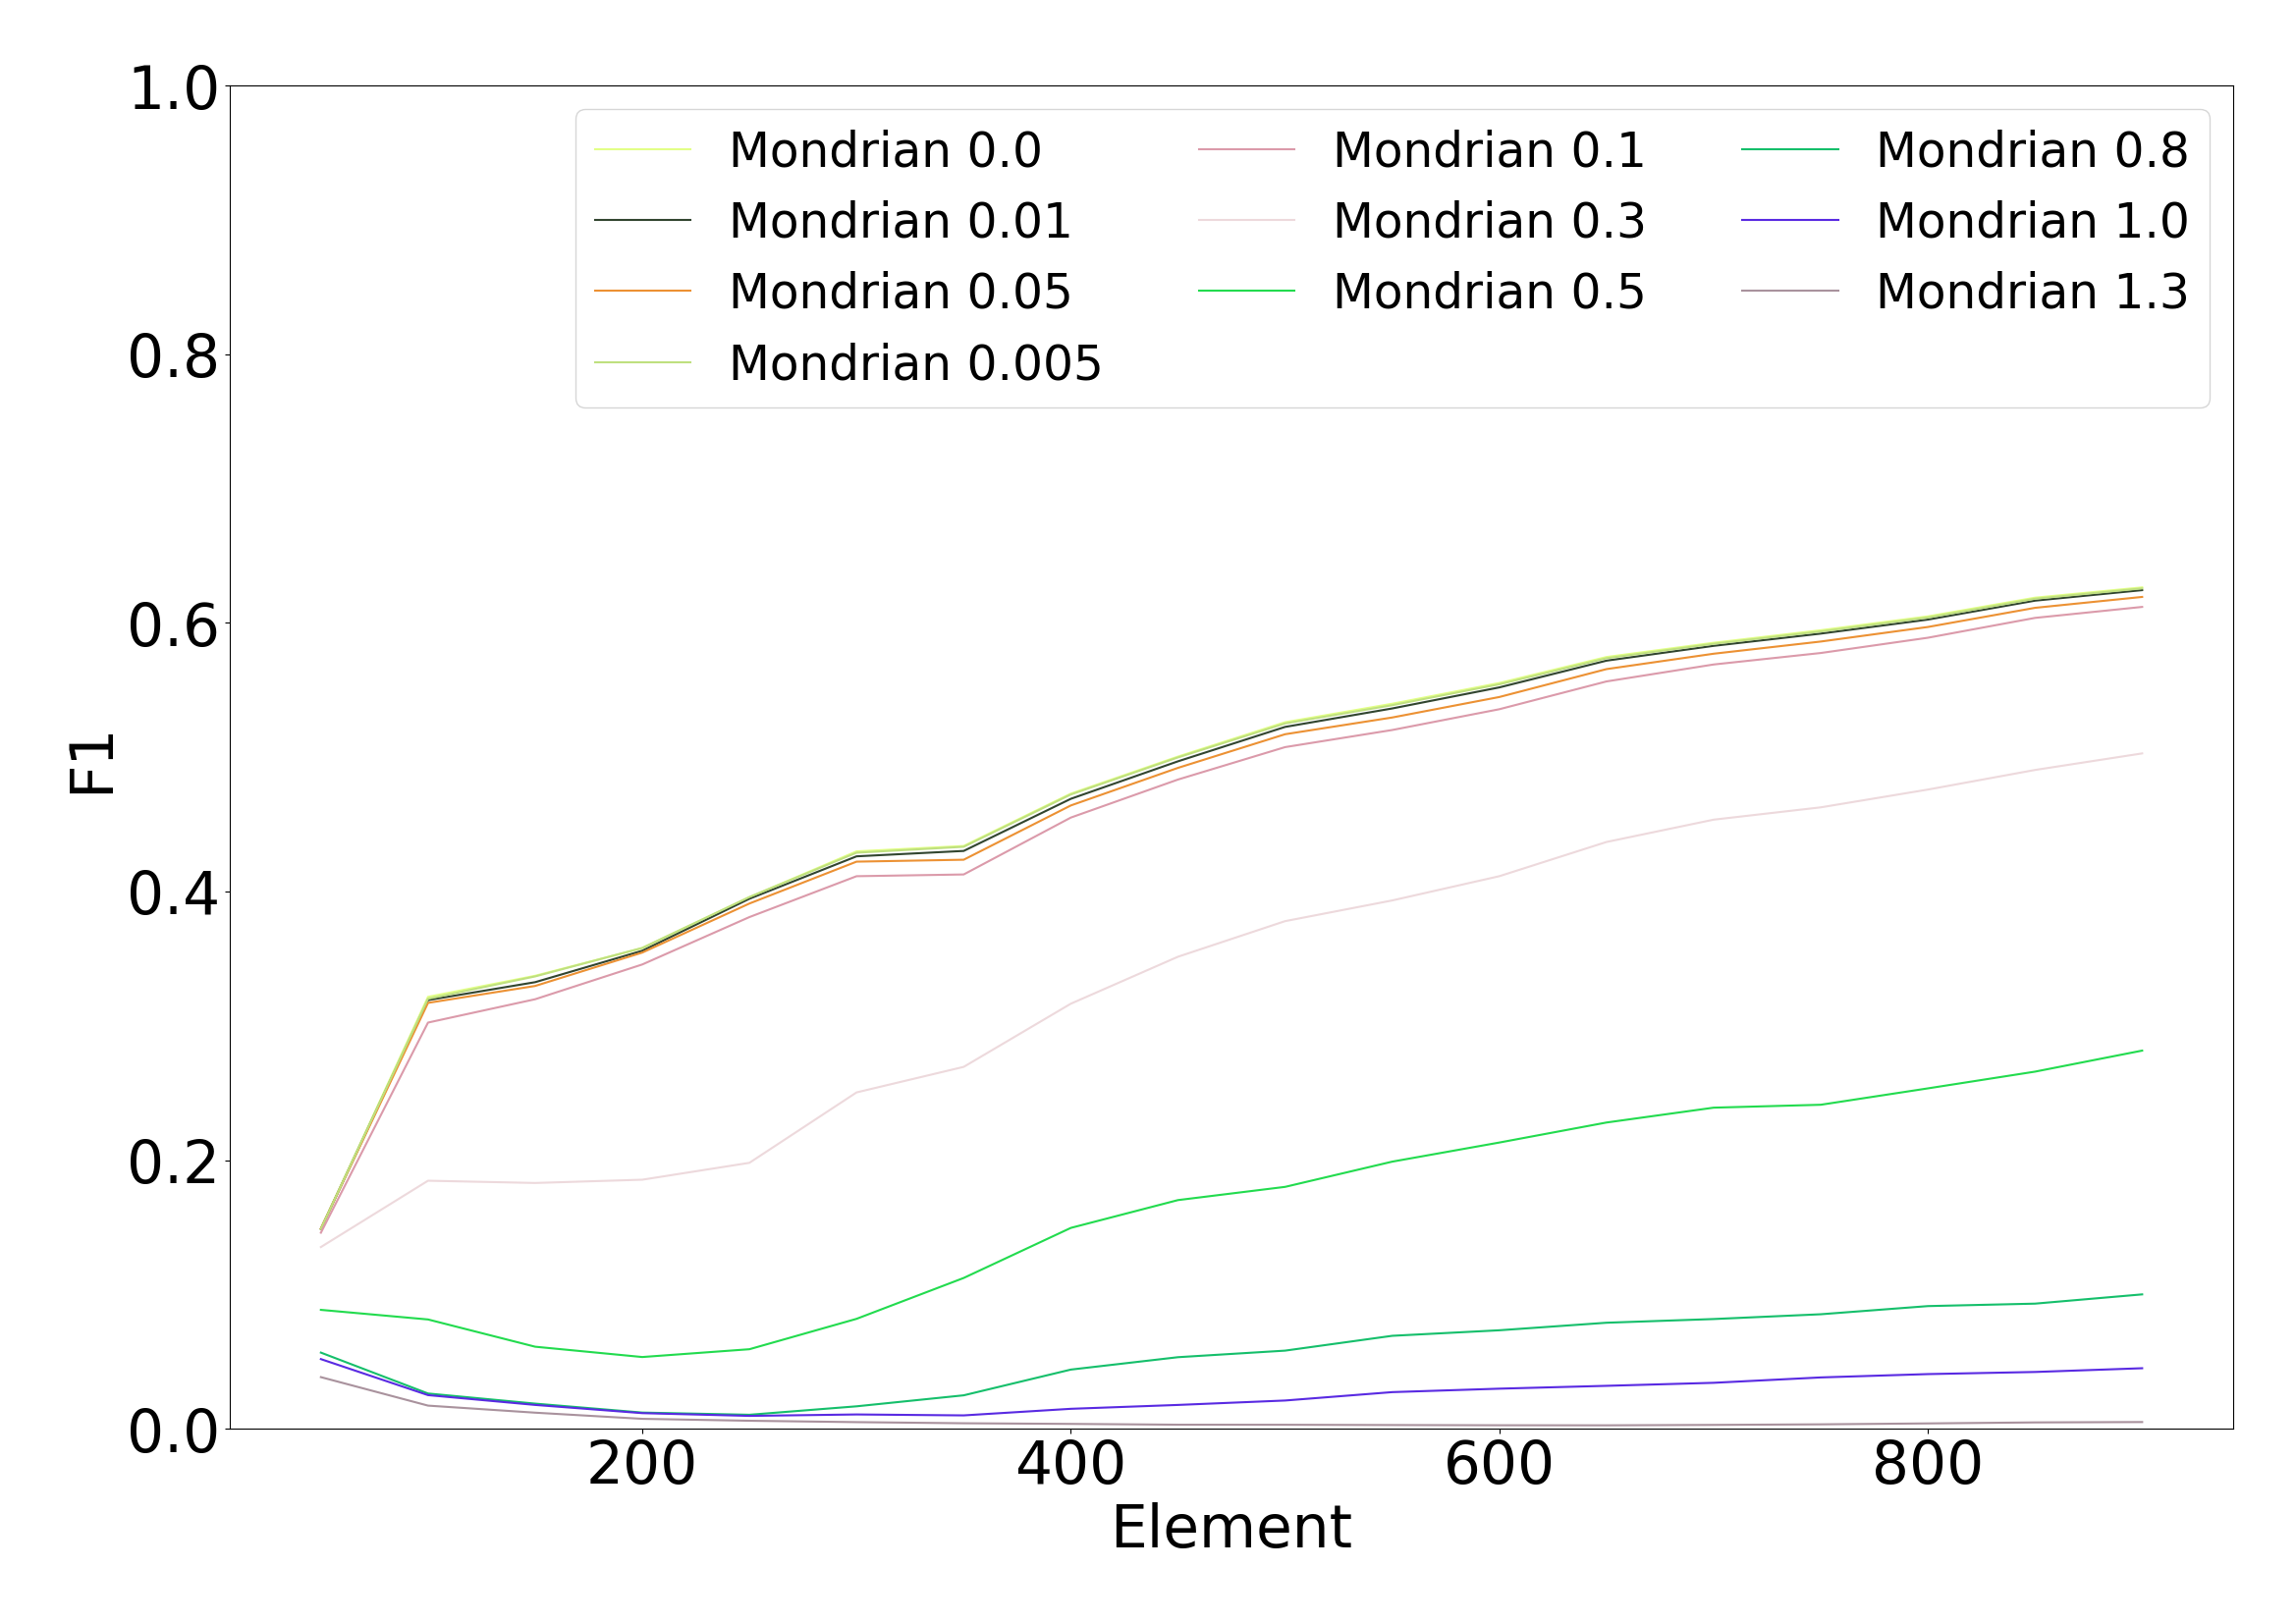
\includegraphics[width=\textwidth]{figures/calibration_mondrian_base.png}
		\caption{Impact of the base count with 10 trees, a budget of $1.0$, and a discount factor of $0.2$.} 
		\label{fig:mondrian-base-count}
	\end{subfigure}
	\hfill
	 \begin{subfigure}[b]{0.49\textwidth}
		 \centering
		 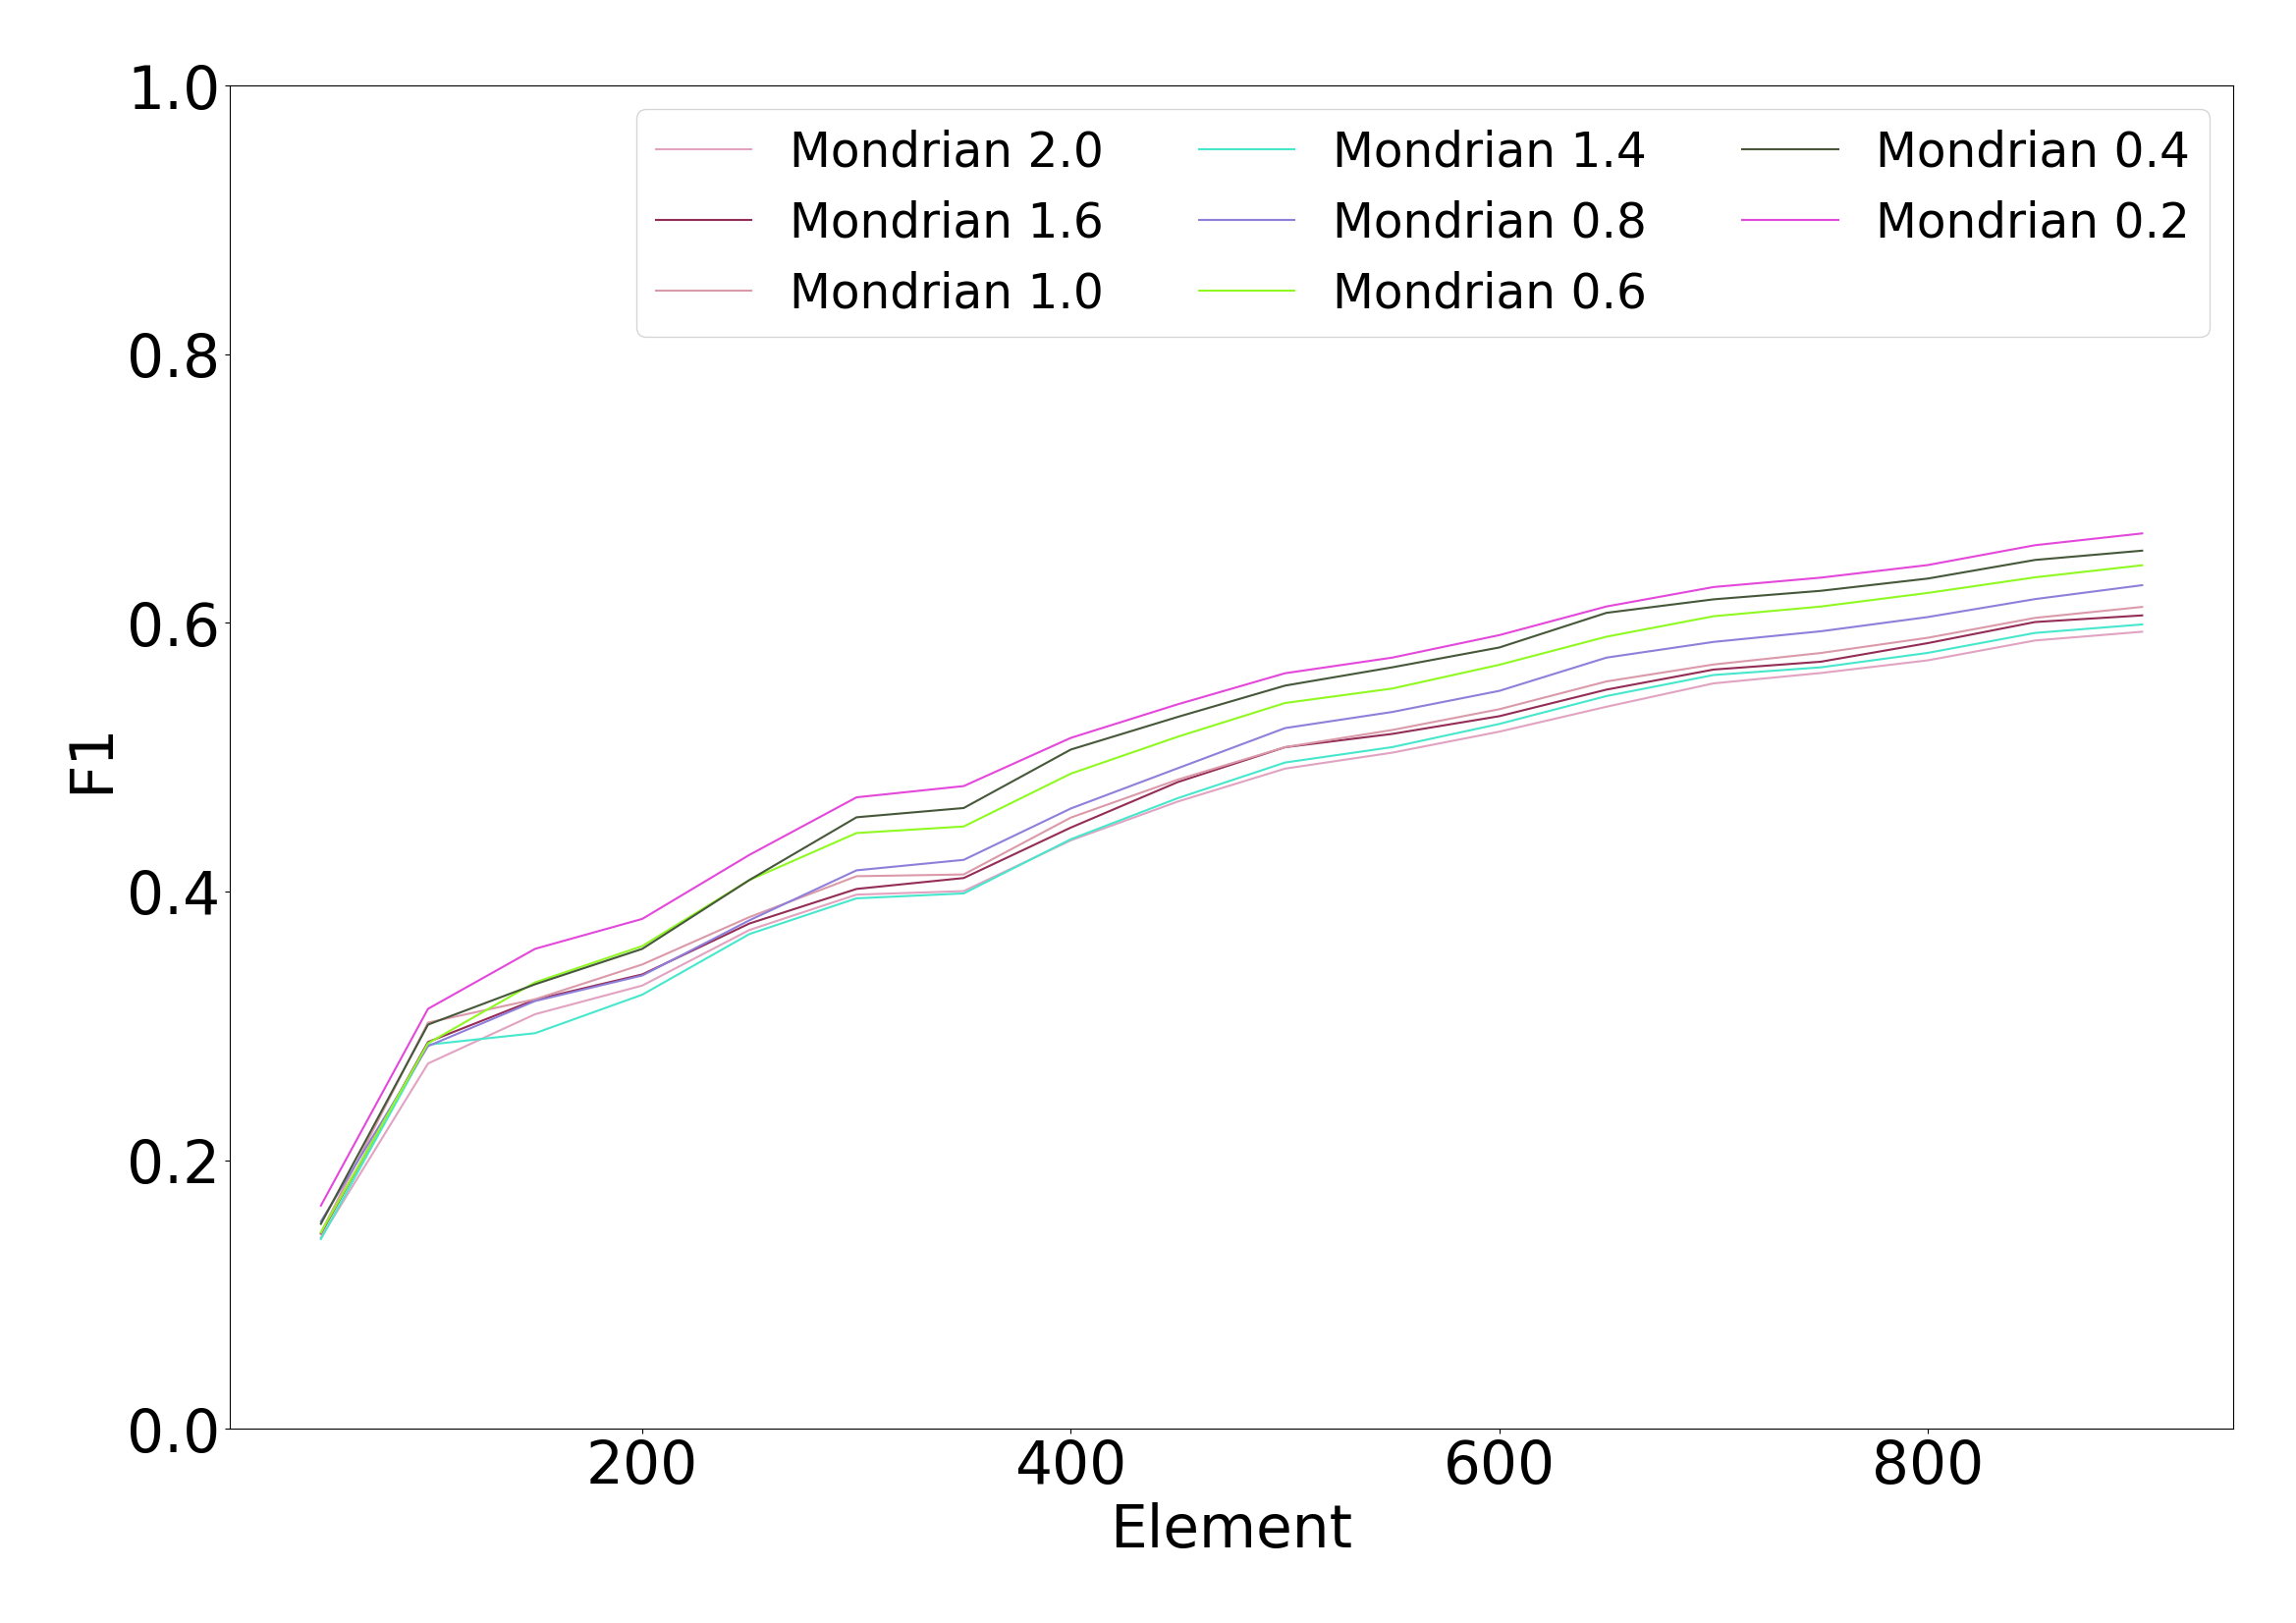
\includegraphics[width=\textwidth]{figures/calibration_mondrian_lifetime.png}
		 \caption{Impact of the budget with 10 trees, a base count of $0.1$, and discount factor of $0.2$.}
		 \label{fig:mondrian-budget}
	 \end{subfigure}
	 \hfill
	 \begin{subfigure}[b]{0.49\textwidth}
		 \centering
		 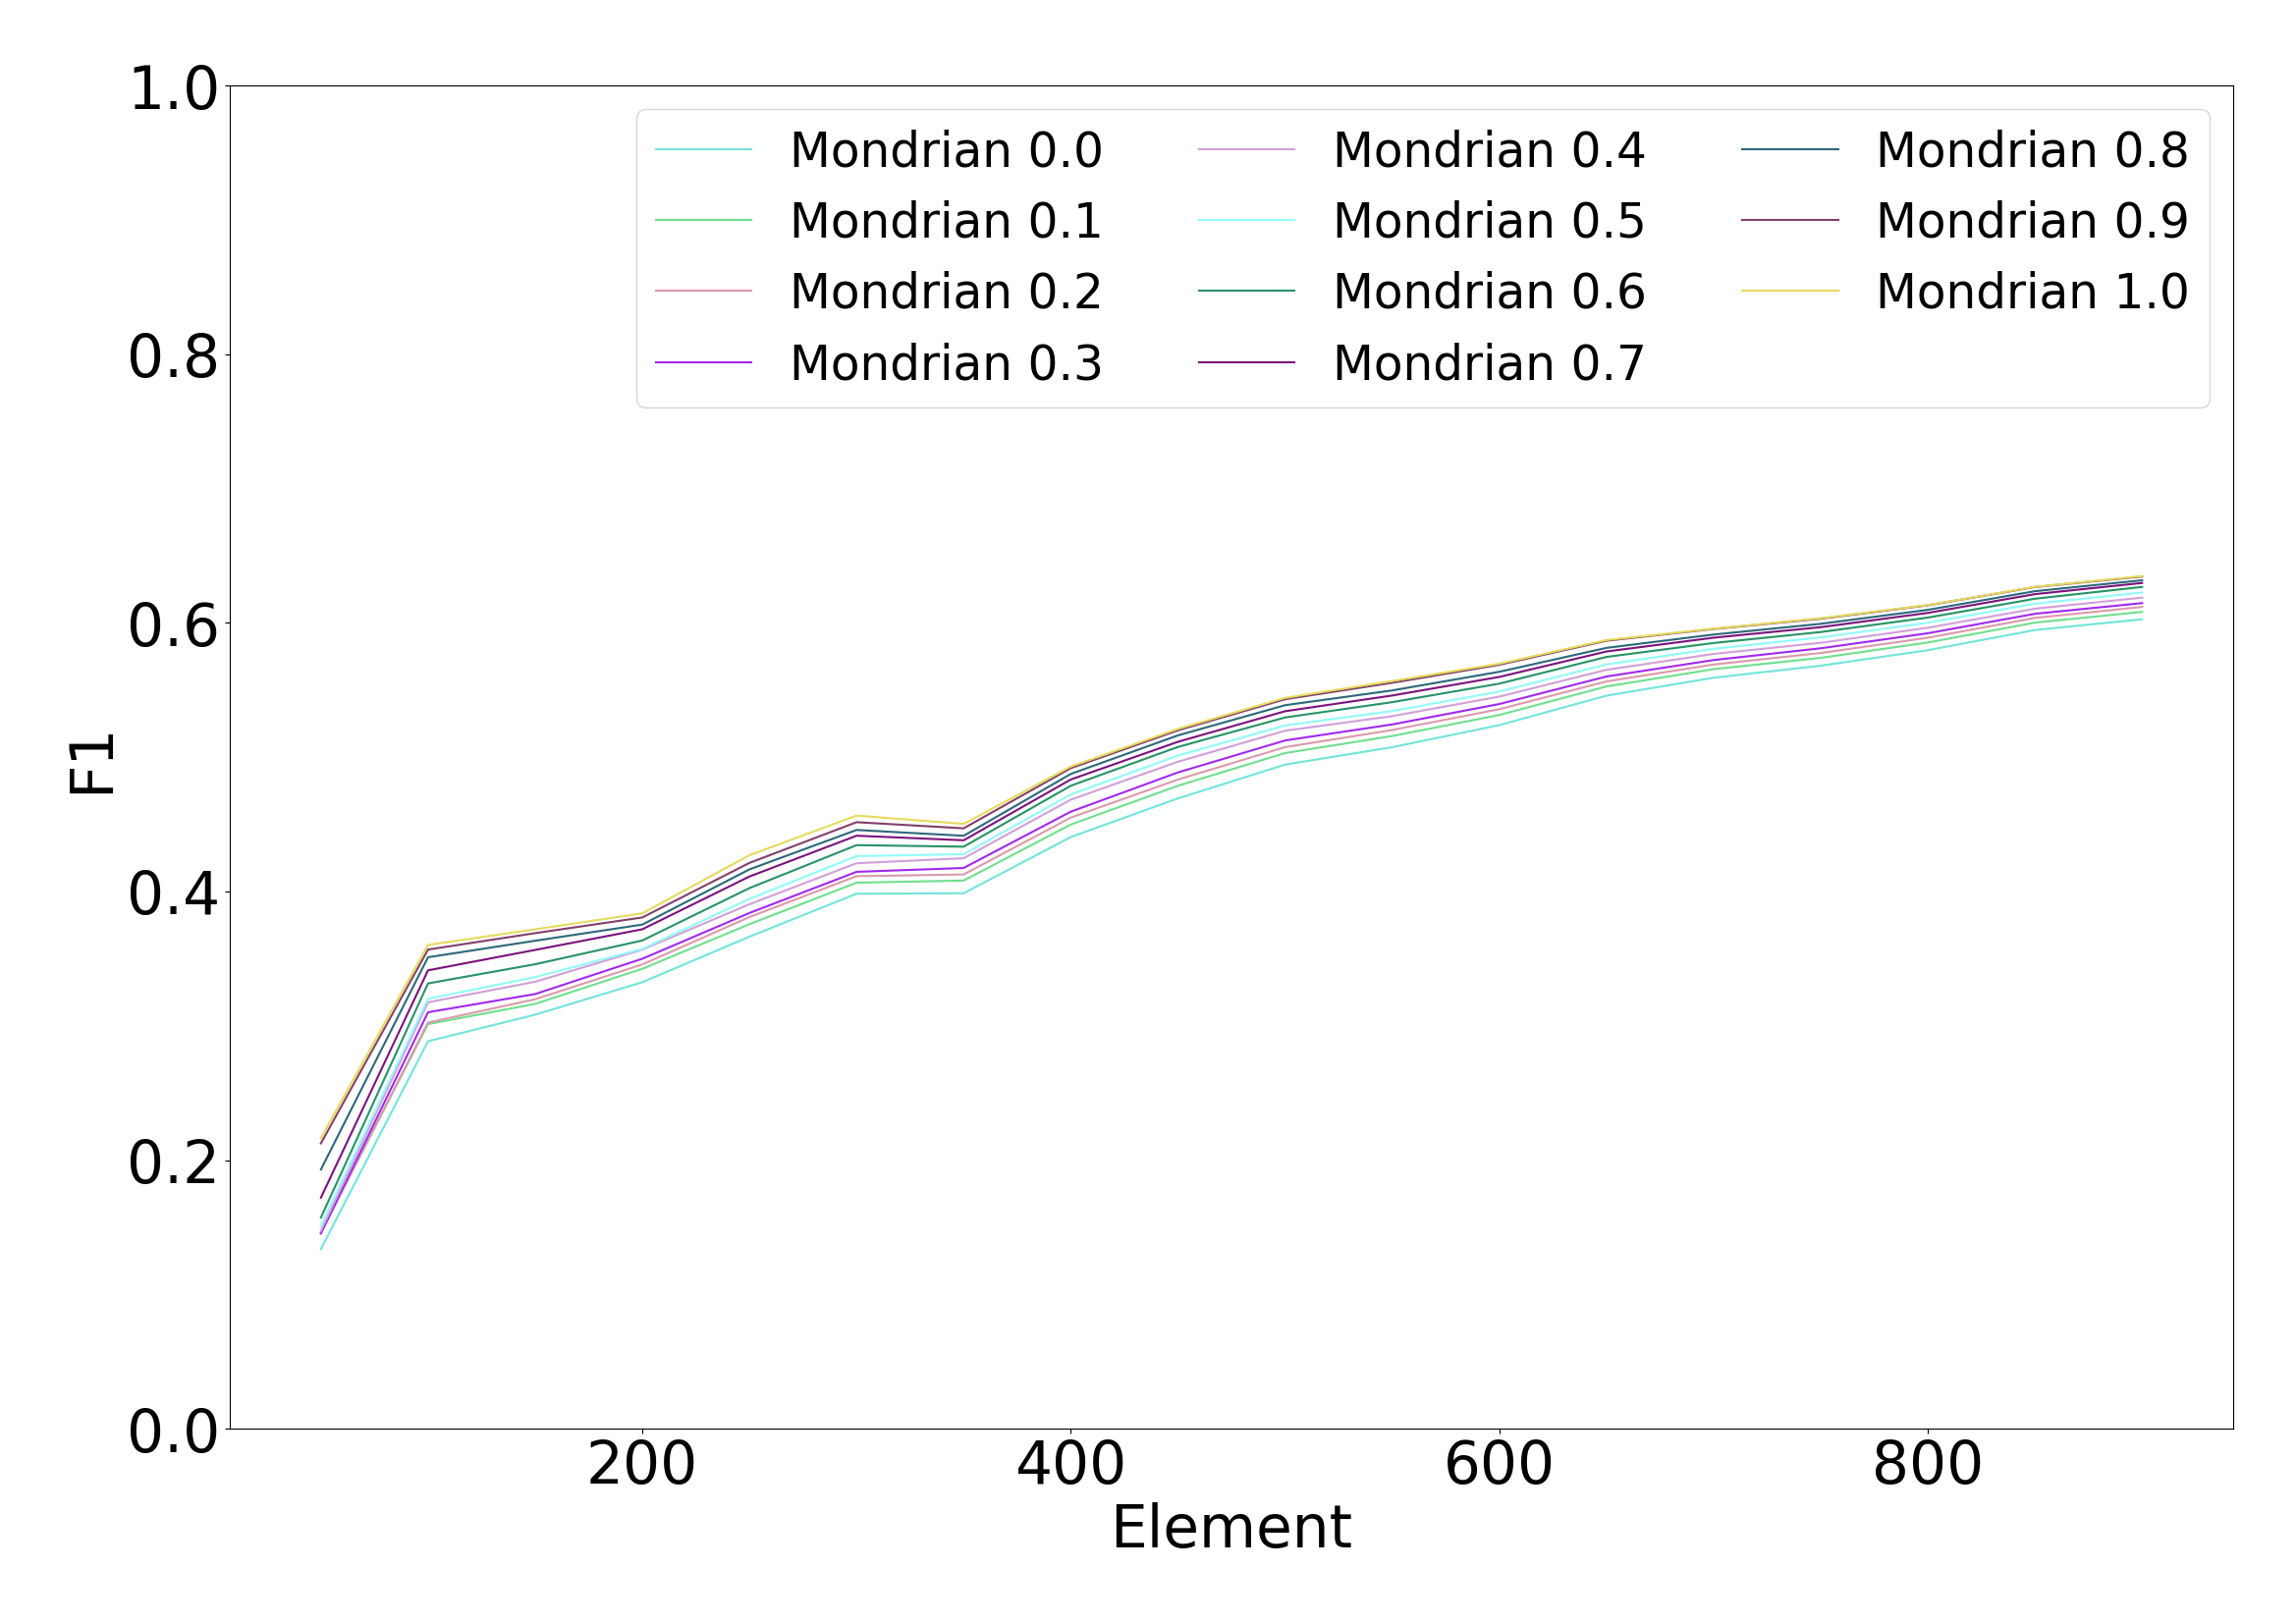
\includegraphics[width=\textwidth]{figures/calibration_mondrian_discount.png}
		 \caption{Impact of the discount factor with 10 trees, a budget of $1.0$, and a base count of $0.1$.}
		 \label{fig:mondrian-discount}
	 \end{subfigure}
		\caption{Hyperparameters tuning for Mondrian with first subject of \banosdataset dataset.}
		\label{fig:mondrian-tuning}
\end{figure}


